\documentclass{beamer}

\mode<presentation>{
\usetheme{Madrid}
%\usecolortheme{beaver}
}
\usepackage[utf8]{inputenc}
%\usepackage{default}
%\usepackage[portuguese]{babel}
%\usepackage{pgfplots}
%\pgfplotsset{/pgf/number format/use comma,compat=newest}
%\usepackage{color}
\usepackage{amsfonts}
\usepackage{mathrsfs}  

%\usepackage{hyperref}


%MEUS COMANDOs

\usepackage{tikz}
\usetikzlibrary{quotes, angles, intersections}
\newcommand{\R}{\mathbb{R}}
\newcommand{\D}{\mathscr{D}}
\newcommand{\Pp}{\mathscr{P}}
\newcommand{\Cc}{\mathscr{C}}
\newcommand{\E}{\mathscr{E}}

\newcommand{\bigO}{\mathscr{O}}
\usetikzlibrary{matrix}
\usepackage{pgfplots}
\pgfplotsset{compat=1.4}
\usepackage{algorithm2e}
\usepackage{algorithmic}
\usepackage{float}
\usepackage{caption}
\newcommand{\source}[1]{\caption*{Source: {#1}} }

%\usepgfplotslibrary{external}
%\tikzexternalize
%\usepackage{natbib}

\usepackage[
backend=biber,
style=authoryear,
autocite=inline
]{biblatex}
%\DeclareLanguageMapping{english}{english-apa}

\addbibresource{../references.bib} %Imports bibliography file
%\DeclareLanguageMapping{american}{american-apa}



%FIM MEUS COMANDOS

\title[Qualificação de Mestrado]{Planar Maximal Covering with Ellipses}
\author[Tedeschi, D. F.]{Danilo F. Tedeschi\\ \small Orientadora: Dra. Marina Andretta}

\institute[ICMC]{Instituto de Ciências Matemáticas e Computação}
\date{\today}

\begin{document}

\begin{frame}
 \maketitle
 
 
\centering Agradecimentos à CAPES.
\end{frame}

\begin{frame}
\frametitle{Contents}
 \tableofcontents
\end{frame}

\section{Introduction}
\begin{frame}
\frametitle{Introduction}
\begin{itemize}
	\item Covering problems
	\begin{itemize}
		\item Minimum Cover Problem \autocite{karp}
		\item Maximal Covering Problem \autocite{church:1974}
	\end{itemize}

\end{itemize}

\begin{figure}
	\caption{Minimum Vertex Cover and its maximal counterpart. The colored edges are in the cover.}
	\documentclass{article}


%% Use the option review to obtain double line spacing
%% \documentclass[preprint,review,12pt]{elsarticle}

%% Use the options 1p,twocolumn; 3p; 3p,twocolumn; 5p; or 5p,twocolumn
%% for a journal layout:
%% \documentclass[final,1p,times]{elsarticle}
%% \documentclass[final,1p,times,twocolumn]{elsarticle}
%% \documentclass[final,3p,times]{elsarticle}
%% \documentclass[final,3p,times,twocolumn]{elsarticle}
%% \documentclass[final,5p,times]{elsarticle}
%% \documentclass[final,5p,times,twocolumn]{elsarticle}

%% The graphicx package provides the includegraphics command.
\usepackage[utf8]{inputenc}
\usepackage{graphicx}
\usepackage{hyperref}
\usepackage{amssymb}
\usepackage{amsmath}
\usepackage{amsthm}
\usepackage{subcaption}
\usepackage{siunitx}
\sisetup{group-separator = {,}}

\usepackage{multirow}

%\journal{EJOR}

\usepackage[mathscr]{eucal}
\newcommand{\R}{\mathbb{R}}
\newcommand{\Co}{\mathbb{Co}}
\newcommand{\D}{\mathscr{D}}
\newcommand{\Pp}{\mathscr{P}}
\newcommand{\Cc}{\mathscr{C}}
\newcommand{\E}{\mathscr{E}}
\newcommand{\F}{\mathscr{F}}
\newcommand{\Ww}{\mathscr{W}}
\newcommand{\Rr}{\mathscr{R}}
\newcommand{\norm}[2][2]{\left\lVert#2\right\rVert_{#1}}
\newcommand{\bigO}{\mathscr{O}}
\newtheorem{thm}{Theorem}
\newtheorem{prp}{Proposition}
\newtheorem{lem}{Lemma}
%\newdefinition{rmk}{Remark}
%\newdefinition{definition}{Definition}
%\newproof{pf}{Proof}
%\renewcommand\qedsymbol{$\blacksquare$}


\RequirePackage{algorithm, algpseudocode}
\renewcommand{\algorithmicrequire}{\textbf{Input:}}
\renewcommand{\algorithmicensure}{\textbf{Output:}}
\newcommand{\algorithmautorefname}{Algorithm}
\newcommand{\definitionautorefname}{Definition}
\newcommand{\thmautorefname}{Theorem}
\newcommand{\prpautorefname}{Proposition}
\newcommand{\lemmaautorefname}{Lemma}
\newcommand{\lemautorefname}{Lemma}
\newcommand{\sigla}[2]{#2 (#1)}
\newcommand{\citeonline}[1]{\cite{#1}}

\begin{document}
		\title{Cover Letter}
		\maketitle

		Dear Editor, we herewith submit the manuscript entitled New Exact Algorithms for Planar Maximum Covering Location by Ellipses Problems addressing two not-vastly-explored problems on which we could only find two published papers, with the most recent one being from seven years ago.
		
		We propose new algorithms for those two problems after proving that if the number of given ellipses is constant, an optimal solution is contained in a polynomial-sized set of solutions, transforming both problems in combinatorial optimization problems. 
		
		We show that significant advances were accomplished both in theory and in practice by our work, and we believe that our manuscript is a strong match for this journal as, besides dealing with an optimization problem that has not been vastly studied, the most recent paper on this subject is published here.
		
		%\section*{References}
		%% New version of the num-names style
		%\bibliographystyle{elsarticle-num}
		%\bibliography{../references}
		
\end{document}
	
	\source{Elaborated by the author.}
\end{figure}
\end{frame}



\begin{frame}{Introduction}
\begin{itemize}

	\item Maximal Covering Location Problem (MCLP)
	
	\begin{itemize}
		\item Introduce at first for networks \autocite{church:1974}. Facilities are placed on nodes, covering a radius of neighboring vertexes.
		
		\item It is a NP-Hard problem \autocite{hatta:2013}.
	\end{itemize}
	\item Planar Maximal Covering Location Problem (PMCLP)
	\begin{itemize}
		\item Introduced by \autocite{church:1984}.
		\item One disk is 3SUM-Hard \autocite{3SUM-kopelowitz:2014}.
		\item One disk: $\bigO(n^2)$ and $\bigO(n^2\log{n})$ algorithms.
		\item $m$ disks: $\bigO(n^{2m-1}\log{n})$ algorithm.
	\end{itemize}
	\item Goals
	\begin{itemize}
		\item Develop a $\bigO(n^2\log{n})$ algorithm for the one disk case.
		\item Adapt it for the $m$ ellipses case creating a $\bigO(n^{2m})$ algorithm.
	\end{itemize}
\end{itemize}

\end{frame} 




%\section{Preliminaries}

%\begin{frame}{Preliminaries}
	
%	\begin{block}{Norms}
%		Let $u \in \R^2$ and $Q$ a $2x2$ positive definite matrix
%		\begin{itemize}
%			\item Euclidean
%			\begin{equation*}
%			||u||_2 = \sqrt{u^Tu}
%			\end{equation*}
%			
%			\item Elliptical
%			\begin{equation*}
%			||u||_{Q} = \sqrt{u^TQu}
%			\end{equation*}
%		\end{itemize}
%	\end{block}

%\end{frame}





\section{Maximal Covering by Disks}
\begin{frame}{Maximal Covering by Disks}{One disk}
	
	$MCD(\Pp, 1)$ is the problem of placing one disk on the plane to cover a subset of a demand set $\Pp$, with $n$ points, maximizing the weights of the covered points.
	
	\begin{equation*}\label{eq:max_one_disk}
		\max_q w(\Pp \cap D(q)),
	\end{equation*}
	
	\begin{itemize}
		\item $\Pp=\{p_1,\dots,p_n\}$ is the demand set with weights $w(p_i)>0$.
		\item $w(A)$, $A\subset \Pp$, is the sum of weights of the points in $A$.
		\item $D(q)$ is a unit disk with center at point $q$.
		%\item \autocite{chazelle:1986} proposed a $\bigO(n^2)$ algorithm
		%\item \autocite{drezner} proposed a $\bigO(n^2\log{n})$ which our work is based on
		%\item We will introduce an equivalent problem...
	\end{itemize}
\end{frame}

\begin{frame}{Maximal Covering by Disks}{One disk}
\begin{figure}
	\caption{An instance of $MCD(\Pp,1)$.}
	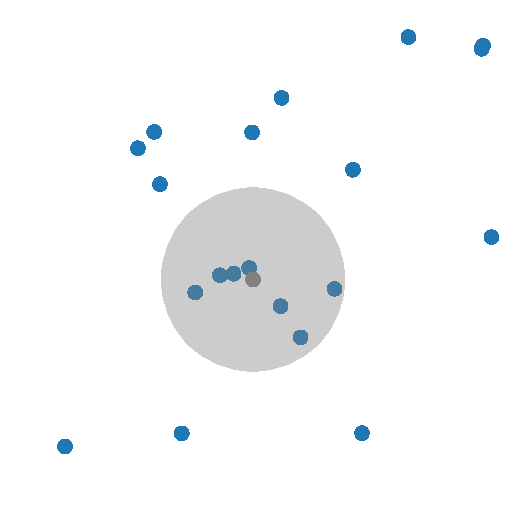
\includegraphics[scale=0.6]{figures/mcd_one_disk.pdf}
	\source{Elaborated by the author.}
\end{figure}
\end{frame}

\begin{frame}{Maximal Covering By Disks}{One disk}
	
	Works and results found in the literature:
	
	\begin{itemize}
		\item $MCD$ is as difficult the problem of given $n$ numbers, find three of them that sum to $0$ (3SUM-HARD). Proved by \autocite{aronov:2008}.
		
		\item In \autocite{drezner} a $\bigO(n^2\log{n})$ algorithm was developed. The idea of our algorithm to sort the intersections by their angles comes from here.
		
		\item In \autocite{chazelle:1986}, a $\bigO(n^2)$ algorithm was developed. It actually solves an equivalent problem which is introduced next.
	\end{itemize}
	
	
	
\end{frame}

\subsection{Maximum Weight Clique Problem}
\begin{frame}{Maximum Weight Clique Problem}
	Let $\D=\{D_1,\dots,D_n\}$ be a set of $n$ unit disks with weights $w_i>0$. The maximum weight clique is defined as
	
	\begin{equation*}
	\max_{q\in\R^2} \sum_{D_k \cap q \neq \emptyset} w_k,
	\end{equation*}
	
	\begin{itemize}
		\item A clique is a non-empty intersection area of a subset of disks. We search for only a point in an optimal clique.
		
		\item The weight of a clique is the sum of the weights of the disks that intersect with it.
		
		\item In our case, we just want a point from the optimum clique.
		
		\item Given an instance $MCD(\Pp, 1)$: fix the disk centers at $\Pp =\{p_1,\dots,p_n\}$ with weights $w_k=w(p_k)$.

		%\item An optimal solution for the maximum weight clique is an optimal solution for $MCD(\Pp,1)$.
	\end{itemize}
\end{frame}

\begin{frame}{Maximum Weight Clique Problem}{Equivalence}
	\begin{figure}
		\only<1>{\caption{An instance of $MCD(\Pp, 1)$. We will show how an instance of the Maximum Weight Clique Problem is constructed from it.}}
		\only<2>{\caption{An instance of the Maximum Weight Clique Problem obtained from an instance of $MCD(\Pp, 1)$.}}
		\only<3>{\caption{An instance of the Maximum Weight Clique Problem obtained from an instance of $MCD(\Pp, 1)$. In gray, the optimal solution.}}
		\only<1>{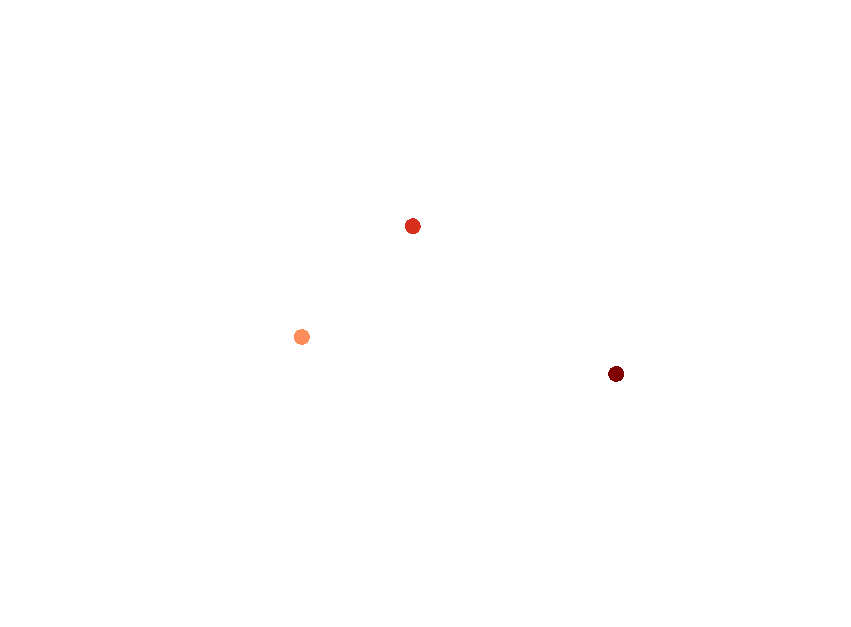
\includegraphics[scale=0.50]{figures/mwc_1.pdf}}
		\only<2>{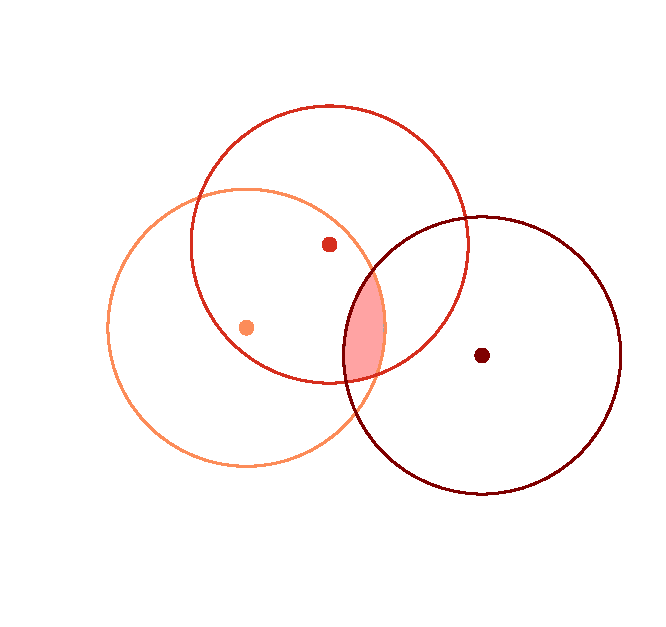
\includegraphics[scale=0.50]{figures/mwc_2.pdf}}
		\only<3>{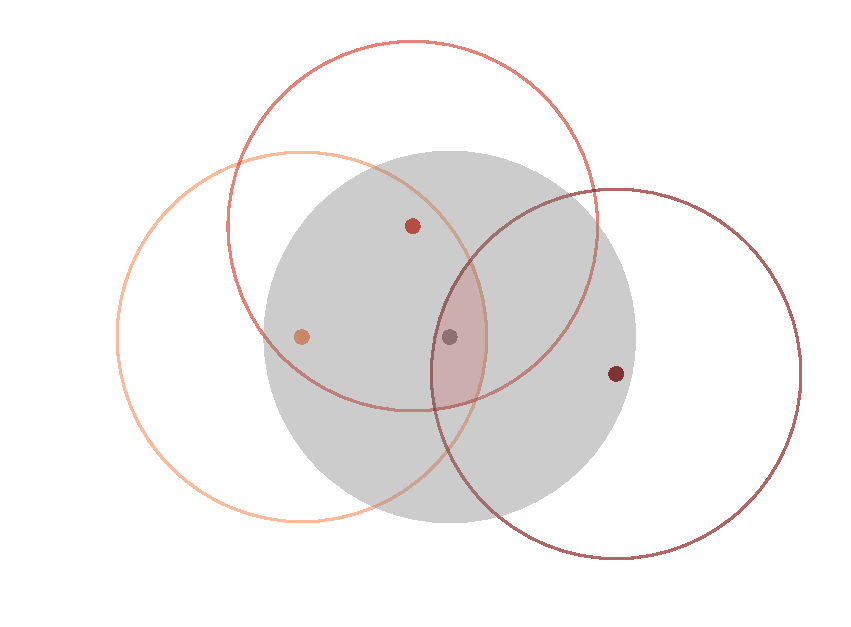
\includegraphics[scale=0.50]{figures/mwc_3.pdf}}
		%\only<2>{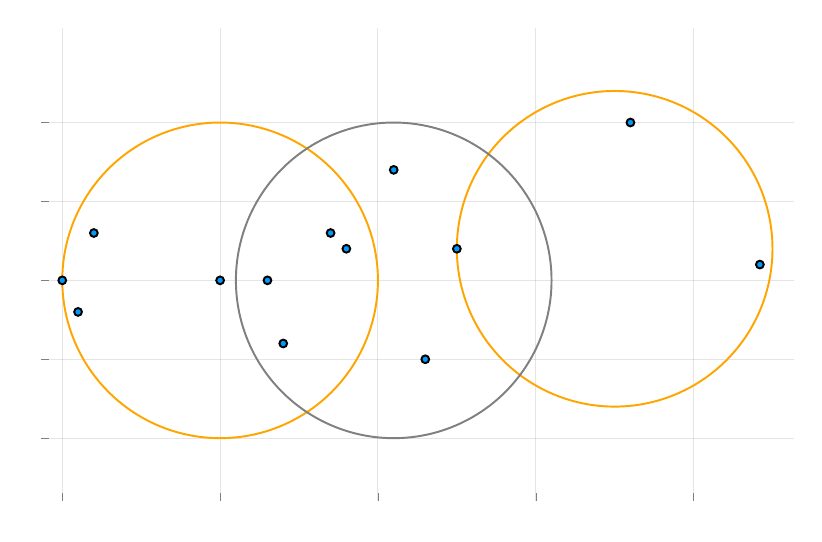
\begin{tikzpicture}[scale=0.7]
\begin{axis}[height = {101.6mm}, axis equal = {true}, ylabel = {}, xmin = {-1.135}, xmax = {3.635}, ymax = {1.2659669777078058}, xlabel = {}, unbounded coords=jump,scaled x ticks = false,xlabel style = {font = {\fontsize{11 pt}{14.3 pt}\selectfont}, color = {rgb,1:red,0.00000000;green,0.00000000;blue,0.00000000}, draw opacity = 1.0, rotate = 0.0},xmajorgrids = true,xtick = {-1.0,0.0,1.0,2.0,3.0},xticklabels = {},xtick align = inside,xticklabel style = {font = {\fontsize{8 pt}{10.4 pt}\selectfont}, color = {rgb,1:red,0.00000000;green,0.00000000;blue,0.00000000}, draw opacity = 1.0, rotate = 0.0},x grid style = {color = {rgb,1:red,0.00000000;green,0.00000000;blue,0.00000000},
draw opacity = 0.1,
line width = 0.5,
solid},axis lines* = left,separate axis lines,x axis line style = {draw opacity = 0},scaled y ticks = false,ylabel style = {font = {\fontsize{11 pt}{14.3 pt}\selectfont}, color = {rgb,1:red,0.00000000;green,0.00000000;blue,0.00000000}, draw opacity = 1.0, rotate = 0.0},ymajorgrids = true,ytick = {-1.0,-0.5,0.0,0.5,1.0},yticklabels = {},ytick align = inside,yticklabel style = {font = {\fontsize{8 pt}{10.4 pt}\selectfont}, color = {rgb,1:red,0.00000000;green,0.00000000;blue,0.00000000}, draw opacity = 1.0, rotate = 0.0},y grid style = {color = {rgb,1:red,0.00000000;green,0.00000000;blue,0.00000000},
draw opacity = 0.1,
line width = 0.5,
solid},axis lines* = left,separate axis lines,y axis line style = {draw opacity = 0},    xshift = 0.0mm,
    yshift = 0.0mm,
    axis background/.style={fill={rgb,1:red,1.00000000;green,1.00000000;blue,1.00000000}}
,legend style = {color = {rgb,1:red,0.00000000;green,0.00000000;blue,0.00000000},
draw opacity = 1.0,
line width = 1,
solid,fill = {rgb,1:red,1.00000000;green,1.00000000;blue,1.00000000},font = {\fontsize{8 pt}{10.4 pt}\selectfont}},colorbar style={title=}, ymin = {-1.0659669777078058}, width = {152.4mm}]\addplot+[draw=none, color = {rgb,1:red,0.00000000;green,0.60560316;blue,0.97868012},
draw opacity = 1.0,
line width = 0,
solid,mark = *,
mark size = 2.0,
mark options = {
    color = {rgb,1:red,0.00000000;green,0.00000000;blue,0.00000000}, draw opacity = 1.0,
    fill = {rgb,1:red,0.00000000;green,0.60560316;blue,0.97868012}, fill opacity = 1.0,
    line width = 1,
    rotate = 0,
    solid
},forget plot] coordinates {
(-1.0, 0.0)
(-0.9, -0.2)
(-0.8, 0.3)
(0.0, 0.0)
(0.3, 0.0)
(0.4, -0.4)
(0.7, 0.3)
(0.8, 0.2)
(1.1, 0.7)
(1.3, -0.5)
(1.5, 0.2)
(3.42, 0.1)
(2.6, 1.0)
};
\addplot+ [color = {rgb,1:red,1.00000000;green,0.64705882;blue,0.00000000},
draw opacity = 1.0,
line width = 1,
solid,mark = none,
mark size = 2.0,
mark options = {
    color = {rgb,1:red,0.00000000;green,0.00000000;blue,0.00000000}, draw opacity = 1.0,
    fill = {rgb,1:red,1.00000000;green,0.64705882;blue,0.00000000}, fill opacity = 1.0,
    line width = 1,
    rotate = 0,
    solid
},forget plot]coordinates {
(1.0, 0.0)
(0.9995015891261738, 0.03156854976481053)
(0.9980068533314934, 0.06310563131267365)
(0.995517282601106, 0.09457980779484494)
(0.9920353585932578, 0.12595970506771756)
(0.9875645521655237, 0.15721404296725078)
(0.9821093199149804, 0.18831166648971787)
(0.9756750997357736, 0.21922157684769134)
(0.9682683053985072, 0.24991296237030836)
(0.959896320156857, 0.2803552292170144)
(0.9505674893877829, 0.3105180318741688)
(0.9402911122726756, 0.3403713034041128)
(0.9290774325277306, 0.3698852854165468)
(0.9169376281927888, 0.3990305577323409)
(0.9038838004888236, 0.4277780677102096)
(0.8899289617551803, 0.45609915920701594)
(0.8750870224785937, 0.48396560114283876)
(0.859372777426912, 0.5113496156423267)
(0.8428018909013506, 0.5382239057242885)
(0.8253908811219762, 0.5645616825119181)
(0.8071571037619854, 0.5903366919365284)
(0.7881187346471924, 0.6155232409081792)
(0.7682947516379708, 0.6400962229271071)
(0.7477049157117092, 0.6640311431104312)
(0.7263697512646394, 0.6873041426091843)
(0.7043105256526722, 0.7098920223913329)
(0.6815492279916339, 0.7317722663670767)
(0.6581085472380377, 0.752923063833377)
(0.6340118495722387, 0.773323331215339)
(0.6092831551065166, 0.7929527330827786)
(0.5839471139413063, 0.8117917024210207)
(0.5580289815934402, 0.8298214601357258)
(0.5315545938209014, 0.8470240337722988)
(0.5045503408691775, 0.8633822754312233)
(0.47704314116488955, 0.8788798788614604)
(0.44906041448292017, 0.8935013957148741)
(0.4206300546137844, 0.9072322509454813)
(0.39178040155849314, 0.9200587573381745)
(0.3625402132786245, 0.9319681291524348)
(0.33293863702976106, 0.942948494867437)
(0.30300518030687273, 0.9529889090158392)
(0.2727696814306032, 0.9620793630944628)
(0.24226227980378318, 0.9702107955409863)
(0.21151338586781906, 0.9773751007667072)
(0.18055365078890231, 0.9835651372363698)
(0.14941393590426094, 0.9887747345870026)
(0.11812528195890805, 0.9929986997786696)
(0.08671887816355095, 0.9962328222710067)
(0.05522603110450817, 0.9984738782203788)
(0.0236781335366241, 0.9997196336934779)
(-0.00789336690971331, 0.9999688468941563)
(-0.0394569990762527, 0.9992212694012756)
(-0.07098129964801578, 0.9974776464163388)
(-0.10243484451661329, 0.9947397160206569)
(-0.13378628010447904, 0.9910102074427921)
(-0.1650043546187991, 0.9862928383380027)
(-0.196057949203978, 0.9805923110824041)
(-0.22691610896159004, 0.9739143080855378)
(-0.2575480738068967, 0.9662654861260218)
(-0.28792330913116637, 0.9576534697159296)
(-0.3180115362392381, 0.9480868435005095)
(-0.34778276253198237, 0.9375751437008251)
(-0.37720731140357594, 0.9261288486078413)
(-0.40625585182378887, 0.9137593681374367)
(-0.434899427575793, 0.9004790324567516)
(-0.4631094861203477, 0.8863010796932087)
(-0.4908579070575935, 0.8712396427384597)
(-0.5181170301580772, 0.855309735160412)
(-0.5448596829350705, 0.8385272362373773)
(-0.5710592077306947, 0.8209088751292626)
(-0.5966894882888559, 0.802472214201578)
(-0.6217249757884951, 0.7832356315188905)
(-0.6461407143112096, 0.7632183025251686)
(-0.6699123657178553, 0.742440180929283)
(-0.6930162339093318, 0.7209219788147163)
(-0.7154292884473712, 0.6986851459933066)
(-0.7371291875117788, 0.6757518486236088)
(-0.7580943001712453, 0.6521449471151868)
(-0.77830372794553, 0.6278879733408583)
(-0.7977373256375193, 0.6030051071796145)
(-0.8163757214143991, 0.5775211524135886)
(-0.8342003361179174, 0.5514615120031076)
(-0.8511934017844945, 0.5248521627644684)
(-0.8673379793567145, 0.4977196294756834)
(-0.8826179755685469, 0.47009095843600296)
(-0.8970181589874635, 0.44199369050557913)
(-0.9105241751974622, 0.4134558336521342)
(-0.9231225611078606, 0.384505835032011)
(-0.9348007583735982, 0.3551725526334286)
(-0.9455471259136671, 0.3254852265102116)
(-0.9553509515151948, 0.29547344963467004)
(-0.9642024625116117, 0.2651671383986787)
(-0.972092835524257, 0.23459650279236888)
(-0.9790142052577144, 0.20379201629015234)
(-0.9849596723401104, 0.17278438547409986)
(-0.9899233102005571, 0.14160451942495159)
(-0.9939001709768878, 0.11028349891127508)
(-0.9968862904477932, 0.0788525454074766)
(-0.9988786919844436, 0.047342989971558204)
(-0.9998753895176573, 0.015786242013637264)
(-0.9998753895176573, -0.015786242013637018)
(-0.9988786919844436, -0.04734298997155796)
(-0.9968862904477932, -0.07885254540747635)
(-0.9939001709768879, -0.11028349891127483)
(-0.9899233102005572, -0.14160451942495134)
(-0.9849596723401105, -0.17278438547409963)
(-0.9790142052577145, -0.20379201629015212)
(-0.972092835524257, -0.23459650279236863)
(-0.9642024625116118, -0.2651671383986785)
(-0.9553509515151949, -0.2954734496346698)
(-0.9455471259136672, -0.3254852265102114)
(-0.9348007583735983, -0.3551725526334284)
(-0.9231225611078607, -0.38450583503201075)
(-0.9105241751974622, -0.41345583365213395)
(-0.8970181589874636, -0.4419936905055789)
(-0.882617975568547, -0.47009095843600274)
(-0.8673379793567146, -0.49771962947568316)
(-0.8511934017844947, -0.5248521627644683)
(-0.8342003361179176, -0.5514615120031073)
(-0.8163757214143992, -0.5775211524135885)
(-0.7977373256375195, -0.6030051071796143)
(-0.7783037279455302, -0.6278879733408581)
(-0.7580943001712456, -0.6521449471151866)
(-0.737129187511779, -0.6757518486236087)
(-0.7154292884473714, -0.6986851459933063)
(-0.693016233909332, -0.7209219788147162)
(-0.6699123657178554, -0.7424401809292829)
(-0.6461407143112101, -0.7632183025251682)
(-0.6217249757884953, -0.7832356315188904)
(-0.5966894882888565, -0.8024722142015775)
(-0.571059207730695, -0.8209088751292625)
(-0.5448596829350704, -0.8385272362373775)
(-0.5181170301580778, -0.8553097351604116)
(-0.49085790705759375, -0.8712396427384596)
(-0.4631094861203483, -0.8863010796932084)
(-0.4348994275757932, -0.9004790324567515)
(-0.40625585182378887, -0.9137593681374367)
(-0.37720731140357633, -0.9261288486078411)
(-0.3477827625319824, -0.9375751437008251)
(-0.3180115362392388, -0.9480868435005093)
(-0.28792330913116665, -0.9576534697159295)
(-0.2575480738068965, -0.9662654861260219)
(-0.22691610896159048, -0.9739143080855377)
(-0.19605794920397804, -0.9805923110824041)
(-0.16500435461879978, -0.9862928383380026)
(-0.13378628010447927, -0.9910102074427921)
(-0.1024348445166131, -0.994739716020657)
(-0.07098129964801624, -0.9974776464163387)
(-0.03945699907625272, -0.9992212694012756)
(-0.007893366909713777, -0.9999688468941563)
(0.023678133536623857, -0.9997196336934779)
(0.05522603110450836, -0.9984738782203788)
(0.08671887816355048, -0.9962328222710067)
(0.11812528195890803, -0.9929986997786696)
(0.14941393590426047, -0.9887747345870026)
(0.1805536507889021, -0.98356513723637)
(0.21151338586781926, -0.9773751007667072)
(0.24226227980378293, -0.9702107955409863)
(0.27276968143060315, -0.9620793630944628)
(0.3030051803068723, -0.9529889090158394)
(0.332938637029761, -0.942948494867437)
(0.3625402132786239, -0.9319681291524351)
(0.3917804015584929, -0.9200587573381745)
(0.42063005461378433, -0.9072322509454813)
(0.4490604144829198, -0.8935013957148743)
(0.47704314116488955, -0.8788798788614604)
(0.5045503408691769, -0.8633822754312237)
(0.5315545938209012, -0.847024033772299)
(0.5580289815934403, -0.8298214601357258)
(0.5839471139413059, -0.8117917024210209)
(0.6092831551065166, -0.7929527330827786)
(0.6340118495722382, -0.7733233312153395)
(0.6581085472380375, -0.7529230638333771)
(0.681549227991634, -0.7317722663670767)
(0.7043105256526719, -0.7098920223913332)
(0.7263697512646393, -0.6873041426091843)
(0.7477049157117087, -0.6640311431104317)
(0.7682947516379706, -0.6400962229271073)
(0.7881187346471925, -0.615523240908179)
(0.8071571037619851, -0.5903366919365287)
(0.8253908811219762, -0.5645616825119181)
(0.8428018909013504, -0.538223905724289)
(0.8593727774269119, -0.5113496156423268)
(0.8750870224785938, -0.48396560114283854)
(0.8899289617551801, -0.45609915920701627)
(0.9038838004888236, -0.42777806771020954)
(0.9169376281927886, -0.3990305577323414)
(0.9290774325277305, -0.36988528541654697)
(0.9402911122726754, -0.3403713034041135)
(0.9505674893877828, -0.3105180318741691)
(0.959896320156857, -0.28035522921701433)
(0.9682683053985071, -0.2499129623703088)
(0.9756750997357736, -0.21922157684769145)
(0.9821093199149803, -0.18831166648971848)
(0.9875645521655236, -0.15721404296725106)
(0.9920353585932579, -0.12595970506771748)
(0.9955172826011058, -0.09457980779484539)
(0.9980068533314933, -0.06310563131267372)
(0.9995015891261737, -0.03156854976481113)
(1.0, -2.4492935982947064e-16)
};
\addplot+ [color = {rgb,1:red,1.00000000;green,0.64705882;blue,0.00000000},
draw opacity = 1.0,
line width = 1,
solid,mark = none,
mark size = 2.0,
mark options = {
    color = {rgb,1:red,0.00000000;green,0.00000000;blue,0.00000000}, draw opacity = 1.0,
    fill = {rgb,1:red,1.00000000;green,0.64705882;blue,0.00000000}, fill opacity = 1.0,
    line width = 1,
    rotate = 0,
    solid
},forget plot]coordinates {
(3.5, 0.2)
(3.499501589126174, 0.23156854976481053)
(3.4980068533314936, 0.26310563131267367)
(3.495517282601106, 0.29457980779484494)
(3.4920353585932578, 0.32595970506771754)
(3.487564552165524, 0.3572140429672508)
(3.48210931991498, 0.3883116664897179)
(3.4756750997357737, 0.41922157684769135)
(3.468268305398507, 0.44991296237030837)
(3.459896320156857, 0.4803552292170144)
(3.450567489387783, 0.5105180318741689)
(3.440291112272676, 0.5403713034041129)
(3.4290774325277305, 0.5698852854165468)
(3.416937628192789, 0.5990305577323409)
(3.4038838004888237, 0.6277780677102096)
(3.38992896175518, 0.656099159207016)
(3.375087022478594, 0.6839656011428388)
(3.3593727774269118, 0.7113496156423267)
(3.3428018909013506, 0.7382239057242885)
(3.3253908811219763, 0.7645616825119181)
(3.3071571037619854, 0.7903366919365284)
(3.2881187346471923, 0.8155232409081792)
(3.2682947516379706, 0.8400962229271072)
(3.2477049157117093, 0.8640311431104313)
(3.2263697512646394, 0.8873041426091843)
(3.204310525652672, 0.9098920223913329)
(3.181549227991634, 0.9317722663670767)
(3.1581085472380375, 0.952923063833377)
(3.1340118495722384, 0.9733233312153391)
(3.1092831551065165, 0.9929527330827785)
(3.0839471139413064, 1.0117917024210208)
(3.05802898159344, 1.0298214601357258)
(3.0315545938209016, 1.047024033772299)
(3.0045503408691774, 1.0633822754312232)
(2.9770431411648897, 1.0788798788614604)
(2.9490604144829202, 1.093501395714874)
(2.920630054613784, 1.1072322509454813)
(2.891780401558493, 1.1200587573381746)
(2.8625402132786246, 1.1319681291524348)
(2.832938637029761, 1.142948494867437)
(2.8030051803068727, 1.1529889090158392)
(2.7727696814306033, 1.1620793630944628)
(2.742262279803783, 1.1702107955409864)
(2.711513385867819, 1.1773751007667073)
(2.6805536507889025, 1.1835651372363698)
(2.6494139359042608, 1.1887747345870026)
(2.6181252819589083, 1.1929986997786697)
(2.586718878163551, 1.1962328222710068)
(2.555226031104508, 1.1984738782203788)
(2.5236781335366243, 1.199719633693478)
(2.4921066330902866, 1.1999688468941563)
(2.4605430009237472, 1.1992212694012756)
(2.429018700351984, 1.1974776464163388)
(2.397565155483387, 1.194739716020657)
(2.366213719895521, 1.1910102074427922)
(2.334995645381201, 1.1862928383380027)
(2.3039420507960218, 1.1805923110824041)
(2.27308389103841, 1.1739143080855379)
(2.2424519261931035, 1.1662654861260218)
(2.212076690868834, 1.1576534697159295)
(2.181988463760762, 1.1480868435005096)
(2.1522172374680175, 1.137575143700825)
(2.122792688596424, 1.1261288486078413)
(2.093744148176211, 1.1137593681374367)
(2.065100572424207, 1.1004790324567517)
(2.0368905138796523, 1.0863010796932087)
(2.0091420929424064, 1.0712396427384596)
(1.981882969841923, 1.055309735160412)
(1.9551403170649295, 1.0385272362373774)
(1.9289407922693051, 1.0209088751292625)
(1.903310511711144, 1.002472214201578)
(1.878275024211505, 0.9832356315188906)
(1.8538592856887903, 0.9632183025251686)
(1.8300876342821448, 0.9424401809292831)
(1.8069837660906682, 0.9209219788147163)
(1.7845707115526288, 0.8986851459933065)
(1.762870812488221, 0.8757518486236089)
(1.7419056998287545, 0.8521449471151867)
(1.72169627205447, 0.8278879733408584)
(1.7022626743624807, 0.8030051071796145)
(1.6836242785856008, 0.7775211524135885)
(1.6657996638820824, 0.7514615120031076)
(1.6488065982155056, 0.7248521627644684)
(1.6326620206432856, 0.6977196294756833)
(1.617382024431453, 0.670090958436003)
(1.6029818410125365, 0.6419936905055792)
(1.5894758248025378, 0.6134558336521342)
(1.5768774388921394, 0.584505835032011)
(1.5651992416264018, 0.5551725526334286)
(1.554452874086333, 0.5254852265102117)
(1.5446490484848052, 0.49547344963467005)
(1.5357975374883883, 0.46516713839867874)
(1.5279071644757432, 0.4345965027923689)
(1.5209857947422856, 0.4037920162901524)
(1.5150403276598896, 0.37278438547409987)
(1.5100766897994429, 0.3416045194249516)
(1.5060998290231122, 0.3102834989112751)
(1.5031137095522067, 0.2788525454074766)
(1.5011213080155565, 0.2473429899715582)
(1.5001246104823427, 0.21578624201363727)
(1.5001246104823427, 0.184213757986363)
(1.5011213080155565, 0.15265701002844206)
(1.5031137095522067, 0.12114745459252366)
(1.5060998290231122, 0.08971650108872518)
(1.5100766897994427, 0.058395480575048675)
(1.5150403276598894, 0.027215614525900378)
(1.5209857947422853, -0.003792016290152106)
(1.5279071644757432, -0.034596502792368616)
(1.535797537488388, -0.06516713839867849)
(1.5446490484848052, -0.0954734496346698)
(1.5544528740863328, -0.12548522651021138)
(1.5651992416264018, -0.15517255263342838)
(1.5768774388921392, -0.18450583503201073)
(1.5894758248025378, -0.21345583365213394)
(1.6029818410125363, -0.2419936905055789)
(1.617382024431453, -0.2700909584360027)
(1.6326620206432854, -0.29771962947568315)
(1.6488065982155053, -0.3248521627644683)
(1.6657996638820824, -0.3514615120031073)
(1.6836242785856008, -0.37752115241358847)
(1.7022626743624805, -0.4030051071796143)
(1.7216962720544697, -0.4278879733408581)
(1.7419056998287545, -0.45214494711518655)
(1.762870812488221, -0.4757518486236087)
(1.7845707115526286, -0.4986851459933063)
(1.806983766090668, -0.5209219788147161)
(1.8300876342821446, -0.5424401809292829)
(1.8538592856887899, -0.5632183025251682)
(1.8782750242115047, -0.5832356315188905)
(1.9033105117111435, -0.6024722142015775)
(1.9289407922693051, -0.6209088751292624)
(1.9551403170649295, -0.6385272362373775)
(1.9818829698419222, -0.6553097351604116)
(2.0091420929424064, -0.6712396427384595)
(2.036890513879652, -0.6863010796932083)
(2.065100572424207, -0.7004790324567516)
(2.093744148176211, -0.7137593681374368)
(2.122792688596424, -0.726128848607841)
(2.1522172374680175, -0.7375751437008251)
(2.1819884637607614, -0.7480868435005092)
(2.2120766908688334, -0.7576534697159294)
(2.2424519261931035, -0.7662654861260219)
(2.2730838910384095, -0.7739143080855377)
(2.3039420507960218, -0.780592311082404)
(2.3349956453812, -0.7862928383380026)
(2.3662137198955207, -0.791010207442792)
(2.397565155483387, -0.7947397160206571)
(2.4290187003519836, -0.7974776464163387)
(2.4605430009237472, -0.7992212694012757)
(2.492106633090286, -0.7999688468941564)
(2.523678133536624, -0.799719633693478)
(2.5552260311045085, -0.7984738782203789)
(2.5867188781635506, -0.7962328222710067)
(2.618125281958908, -0.7929986997786695)
(2.6494139359042603, -0.7887747345870026)
(2.680553650788902, -0.7835651372363699)
(2.711513385867819, -0.7773751007667071)
(2.742262279803783, -0.7702107955409863)
(2.7727696814306033, -0.7620793630944629)
(2.8030051803068723, -0.7529889090158395)
(2.832938637029761, -0.742948494867437)
(2.8625402132786237, -0.7319681291524351)
(2.891780401558493, -0.7200587573381745)
(2.920630054613784, -0.7072322509454814)
(2.94906041448292, -0.6935013957148743)
(2.9770431411648897, -0.6788798788614603)
(3.004550340869177, -0.6633822754312237)
(3.031554593820901, -0.647024033772299)
(3.0580289815934405, -0.6298214601357257)
(3.083947113941306, -0.6117917024210209)
(3.1092831551065165, -0.5929527330827786)
(3.1340118495722384, -0.5733233312153394)
(3.1581085472380375, -0.5529230638333771)
(3.181549227991634, -0.5317722663670768)
(3.204310525652672, -0.5098920223913332)
(3.2263697512646394, -0.48730414260918425)
(3.247704915711709, -0.46403114311043164)
(3.2682947516379706, -0.4400962229271073)
(3.2881187346471927, -0.415523240908179)
(3.307157103761985, -0.3903366919365287)
(3.3253908811219763, -0.36456168251191806)
(3.3428018909013506, -0.338223905724289)
(3.3593727774269118, -0.3113496156423268)
(3.375087022478594, -0.28396560114283853)
(3.38992896175518, -0.25609915920701626)
(3.4038838004888237, -0.22777806771020953)
(3.4169376281927883, -0.1990305577323414)
(3.4290774325277305, -0.16988528541654696)
(3.4402911122726754, -0.14037130340411347)
(3.4505674893877827, -0.11051803187416909)
(3.459896320156857, -0.08035522921701432)
(3.468268305398507, -0.04991296237030879)
(3.4756750997357737, -0.019221576847691435)
(3.48210931991498, 0.011688333510281534)
(3.487564552165524, 0.042785957032748956)
(3.4920353585932578, 0.07404029493228254)
(3.4955172826011056, 0.10542019220515463)
(3.498006853331493, 0.1368943686873263)
(3.4995015891261736, 0.16843145023518888)
(3.5, 0.19999999999999976)
};
\addplot+ [color = {rgb,1:red,0.50196078;green,0.50196078;blue,0.50196078},
draw opacity = 1.0,
line width = 1,
solid,mark = none,
mark size = 2.0,
mark options = {
    color = {rgb,1:red,0.00000000;green,0.00000000;blue,0.00000000}, draw opacity = 1.0,
    fill = {rgb,1:red,0.50196078;green,0.50196078;blue,0.50196078}, fill opacity = 1.0,
    line width = 1,
    rotate = 0,
    solid
},forget plot]coordinates {
(2.1, 0.0)
(2.0995015891261737, 0.03156854976481053)
(2.0980068533314933, 0.06310563131267365)
(2.095517282601106, 0.09457980779484494)
(2.092035358593258, 0.12595970506771756)
(2.087564552165524, 0.15721404296725078)
(2.0821093199149807, 0.18831166648971787)
(2.075675099735774, 0.21922157684769134)
(2.068268305398507, 0.24991296237030836)
(2.059896320156857, 0.2803552292170144)
(2.0505674893877828, 0.3105180318741688)
(2.0402911122726755, 0.3403713034041128)
(2.0290774325277305, 0.3698852854165468)
(2.016937628192789, 0.3990305577323409)
(2.0038838004888238, 0.4277780677102096)
(1.9899289617551803, 0.45609915920701594)
(1.975087022478594, 0.48396560114283876)
(1.959372777426912, 0.5113496156423267)
(1.9428018909013507, 0.5382239057242885)
(1.9253908811219764, 0.5645616825119181)
(1.9071571037619854, 0.5903366919365284)
(1.8881187346471924, 0.6155232409081792)
(1.8682947516379709, 0.6400962229271071)
(1.8477049157117094, 0.6640311431104312)
(1.8263697512646395, 0.6873041426091843)
(1.8043105256526721, 0.7098920223913329)
(1.781549227991634, 0.7317722663670767)
(1.7581085472380378, 0.752923063833377)
(1.7340118495722388, 0.773323331215339)
(1.7092831551065166, 0.7929527330827786)
(1.6839471139413065, 0.8117917024210207)
(1.6580289815934401, 0.8298214601357258)
(1.6315545938209015, 0.8470240337722988)
(1.6045503408691775, 0.8633822754312233)
(1.5770431411648898, 0.8788798788614604)
(1.5490604144829203, 0.8935013957148741)
(1.5206300546137845, 0.9072322509454813)
(1.4917804015584932, 0.9200587573381745)
(1.4625402132786247, 0.9319681291524348)
(1.4329386370297612, 0.942948494867437)
(1.4030051803068728, 0.9529889090158392)
(1.3727696814306034, 0.9620793630944628)
(1.3422622798037833, 0.9702107955409863)
(1.3115133858678192, 0.9773751007667072)
(1.2805536507889024, 0.9835651372363698)
(1.249413935904261, 0.9887747345870026)
(1.2181252819589081, 0.9929986997786696)
(1.1867188781635511, 0.9962328222710067)
(1.1552260311045082, 0.9984738782203788)
(1.1236781335366242, 0.9997196336934779)
(1.0921066330902869, 0.9999688468941563)
(1.0605430009237473, 0.9992212694012756)
(1.0290187003519844, 0.9974776464163388)
(0.9975651554833868, 0.9947397160206569)
(0.9662137198955211, 0.9910102074427921)
(0.934995645381201, 0.9862928383380027)
(0.9039420507960221, 0.9805923110824041)
(0.87308389103841, 0.9739143080855378)
(0.8424519261931034, 0.9662654861260218)
(0.8120766908688337, 0.9576534697159296)
(0.7819884637607619, 0.9480868435005095)
(0.7522172374680177, 0.9375751437008251)
(0.7227926885964242, 0.9261288486078413)
(0.6937441481762112, 0.9137593681374367)
(0.6651005724242072, 0.9004790324567516)
(0.6368905138796523, 0.8863010796932087)
(0.6091420929424065, 0.8712396427384597)
(0.5818829698419229, 0.855309735160412)
(0.5551403170649296, 0.8385272362373773)
(0.5289407922693053, 0.8209088751292626)
(0.5033105117111442, 0.802472214201578)
(0.47827502421150503, 0.7832356315188905)
(0.4538592856887905, 0.7632183025251686)
(0.4300876342821448, 0.742440180929283)
(0.40698376609066833, 0.7209219788147163)
(0.3845707115526289, 0.6986851459933066)
(0.3628708124882213, 0.6757518486236088)
(0.34190569982875474, 0.6521449471151868)
(0.32169627205447004, 0.6278879733408583)
(0.3022626743624808, 0.6030051071796145)
(0.283624278585601, 0.5775211524135886)
(0.26579966388208265, 0.5514615120031076)
(0.24880659821550555, 0.5248521627644684)
(0.23266202064328556, 0.4977196294756834)
(0.21738202443145316, 0.47009095843600296)
(0.20298184101253658, 0.44199369050557913)
(0.18947582480253788, 0.4134558336521342)
(0.17687743889213947, 0.384505835032011)
(0.16519924162640187, 0.3551725526334286)
(0.15445287408633301, 0.3254852265102116)
(0.1446490484848053, 0.29547344963467004)
(0.1357975374883884, 0.2651671383986787)
(0.12790716447574313, 0.23459650279236888)
(0.12098579474228566, 0.20379201629015234)
(0.1150403276598897, 0.17278438547409986)
(0.11007668979944296, 0.14160451942495159)
(0.10609982902311232, 0.11028349891127508)
(0.10311370955220689, 0.0788525454074766)
(0.10112130801555652, 0.047342989971558204)
(0.10012461048234278, 0.015786242013637264)
(0.10012461048234278, -0.015786242013637018)
(0.10112130801555652, -0.04734298997155796)
(0.10311370955220689, -0.07885254540747635)
(0.10609982902311221, -0.11028349891127483)
(0.11007668979944285, -0.14160451942495134)
(0.11504032765988959, -0.17278438547409963)
(0.12098579474228555, -0.20379201629015212)
(0.12790716447574313, -0.23459650279236863)
(0.1357975374883883, -0.2651671383986785)
(0.1446490484848052, -0.2954734496346698)
(0.1544528740863329, -0.3254852265102114)
(0.16519924162640176, -0.3551725526334284)
(0.17687743889213936, -0.38450583503201075)
(0.18947582480253788, -0.41345583365213395)
(0.20298184101253647, -0.4419936905055789)
(0.21738202443145305, -0.47009095843600274)
(0.23266202064328545, -0.49771962947568316)
(0.24880659821550544, -0.5248521627644683)
(0.26579966388208254, -0.5514615120031073)
(0.2836242785856009, -0.5775211524135885)
(0.30226267436248055, -0.6030051071796143)
(0.32169627205446993, -0.6278879733408581)
(0.3419056998287545, -0.6521449471151866)
(0.36287081248822106, -0.6757518486236087)
(0.3845707115526287, -0.6986851459933063)
(0.4069837660906681, -0.7209219788147162)
(0.4300876342821447, -0.7424401809292829)
(0.45385928568878997, -0.7632183025251682)
(0.4782750242115048, -0.7832356315188904)
(0.5033105117111436, -0.8024722142015775)
(0.5289407922693051, -0.8209088751292625)
(0.5551403170649297, -0.8385272362373775)
(0.5818829698419223, -0.8553097351604116)
(0.6091420929424063, -0.8712396427384596)
(0.6368905138796518, -0.8863010796932084)
(0.665100572424207, -0.9004790324567515)
(0.6937441481762112, -0.9137593681374367)
(0.7227926885964238, -0.9261288486078411)
(0.7522172374680176, -0.9375751437008251)
(0.7819884637607613, -0.9480868435005093)
(0.8120766908688335, -0.9576534697159295)
(0.8424519261931036, -0.9662654861260219)
(0.8730838910384096, -0.9739143080855377)
(0.9039420507960221, -0.9805923110824041)
(0.9349956453812003, -0.9862928383380026)
(0.9662137198955209, -0.9910102074427921)
(0.997565155483387, -0.994739716020657)
(1.029018700351984, -0.9974776464163387)
(1.0605430009237473, -0.9992212694012756)
(1.0921066330902862, -0.9999688468941563)
(1.123678133536624, -0.9997196336934779)
(1.1552260311045084, -0.9984738782203788)
(1.1867188781635505, -0.9962328222710067)
(1.2181252819589081, -0.9929986997786696)
(1.2494139359042606, -0.9887747345870026)
(1.2805536507889022, -0.98356513723637)
(1.3115133858678194, -0.9773751007667072)
(1.342262279803783, -0.9702107955409863)
(1.3727696814306032, -0.9620793630944628)
(1.4030051803068724, -0.9529889090158394)
(1.432938637029761, -0.942948494867437)
(1.462540213278624, -0.9319681291524351)
(1.491780401558493, -0.9200587573381745)
(1.5206300546137843, -0.9072322509454813)
(1.5490604144829199, -0.8935013957148743)
(1.5770431411648898, -0.8788798788614604)
(1.604550340869177, -0.8633822754312237)
(1.6315545938209013, -0.847024033772299)
(1.6580289815934404, -0.8298214601357258)
(1.683947113941306, -0.8117917024210209)
(1.7092831551065166, -0.7929527330827786)
(1.7340118495722383, -0.7733233312153395)
(1.7581085472380376, -0.7529230638333771)
(1.781549227991634, -0.7317722663670767)
(1.8043105256526721, -0.7098920223913332)
(1.8263697512646395, -0.6873041426091843)
(1.847704915711709, -0.6640311431104317)
(1.8682947516379707, -0.6400962229271073)
(1.8881187346471926, -0.615523240908179)
(1.9071571037619852, -0.5903366919365287)
(1.9253908811219764, -0.5645616825119181)
(1.9428018909013505, -0.538223905724289)
(1.9593727774269118, -0.5113496156423268)
(1.975087022478594, -0.48396560114283854)
(1.9899289617551803, -0.45609915920701627)
(2.0038838004888238, -0.42777806771020954)
(2.016937628192789, -0.3990305577323414)
(2.0290774325277305, -0.36988528541654697)
(2.0402911122726755, -0.3403713034041135)
(2.0505674893877828, -0.3105180318741691)
(2.059896320156857, -0.28035522921701433)
(2.068268305398507, -0.2499129623703088)
(2.075675099735774, -0.21922157684769145)
(2.0821093199149803, -0.18831166648971848)
(2.0875645521655235, -0.15721404296725106)
(2.092035358593258, -0.12595970506771748)
(2.095517282601106, -0.09457980779484539)
(2.0980068533314933, -0.06310563131267372)
(2.0995015891261737, -0.03156854976481113)
(2.1, -2.4492935982947064e-16)
};
\end{axis}

\end{tikzpicture}
}
		\source{Elaborated by the author.}
	\end{figure}
\end{frame}

%\begin{frame}{Maximum Weight Clique Problem}{Equivalence}
%		\begin{figure}[H]
%		\centering
		
%		\only<1>{}
		
%		\only<2>{\caption{An instance of the Maximum Weight Clique Problem obtained from an instance of $MCD(\Pp, 1)$. In gray, the optimal solution.}}
		
%		\only<1>{% This file was created by matplotlib2tikz v0.7.4.
\begin{tikzpicture}

\begin{axis}[
tick align=outside,
tick pos=left,
x grid style={white!69.01960784313725!black},
xmin=-2, xmax=2,
xtick style={color=black},
y grid style={white!69.01960784313725!black},
ymin=-2, ymax=2,
ytick style={color=black}
]
\addplot [only marks, draw=red, fill=red, colormap/viridis]
table{%
	x                      y
	-0.8 -0.2
	-0.2 0.4
	0.9 -0.4
};
\path [draw=black, fill=red, opacity=0.2]
(axis cs:0.2,-0.2)
--(axis cs:0.195184726672197,-0.298017140329561)
--(axis cs:0.18078528040323,-0.395090322016128)
--(axis cs:0.156940335732209,-0.490284677254462)
--(axis cs:0.139375395780243,-0.539375395780243)
--(axis cs:0.0902846772544636,-0.556940335732208)
--(axis cs:-0.00490967798387038,-0.58078528040323)
--(axis cs:-0.0812279586139392,-0.59210602792772)
--(axis cs:-0.0951847266721968,-0.498017140329562)
--(axis cs:-0.1,-0.400000000000001)
--(axis cs:-0.0951847266721969,-0.30198285967044)
--(axis cs:-0.0807852804032306,-0.204909677983873)
--(axis cs:-0.056940335732209,-0.109715322745538)
--(axis cs:-0.0238795325112869,-0.0173165676349108)
--(axis cs:0.0180787356516448,0.0713967368259972)
--(axis cs:0.0685303876974546,0.155570233019602)
--(axis cs:0.110157019435624,0.211697248562716)
--(axis cs:0.123879532511284,0.182683432365096)
--(axis cs:0.156940335732207,0.0902846772544693)
--(axis cs:0.180785280403229,-0.00490967798386432)
--(axis cs:0.195184726672196,-0.101982859670432)
--(axis cs:0.2,-0.199999999999992)
--(axis cs:0.2,-0.2);
\draw (-0.8,-0.2) circle (1);
\draw (axis cs:-0.2,0.4) circle (1);
\draw(axis cs:0.9,-0.4) circle (1);
\end{axis}

\end{tikzpicture}}
%		\only<2>{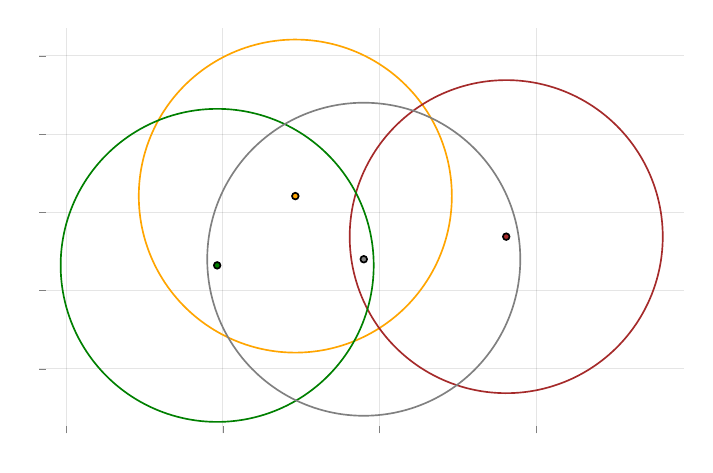
\begin{tikzpicture}[scale=0.6]
\begin{axis}[height = {101.6mm}, axis equal = {true}, ylabel = {}, xmin = {-0.15165998854733476}, xmax = {3.925522135163323}, ymax = {2.176713972397551}, xlabel = {}, unbounded coords=jump,scaled x ticks = false,xlabel style = {font = {\fontsize{11 pt}{14.3 pt}\selectfont}, color = {rgb,1:red,0.00000000;green,0.00000000;blue,0.00000000}, draw opacity = 1.0, rotate = 0.0},xmajorgrids = true,xtick = {0.0,1.0,2.0,3.0},xticklabels = {},xtick align = inside,xticklabel style = {font = {\fontsize{8 pt}{10.4 pt}\selectfont}, color = {rgb,1:red,0.00000000;green,0.00000000;blue,0.00000000}, draw opacity = 1.0, rotate = 0.0},x grid style = {color = {rgb,1:red,0.00000000;green,0.00000000;blue,0.00000000},
draw opacity = 0.1,
line width = 0.5,
solid},axis lines* = left,separate axis lines,x axis line style = {draw opacity = 0},scaled y ticks = false,ylabel style = {font = {\fontsize{11 pt}{14.3 pt}\selectfont}, color = {rgb,1:red,0.00000000;green,0.00000000;blue,0.00000000}, draw opacity = 1.0, rotate = 0.0},ymajorgrids = true,ytick = {0.0,0.5,1.0,1.5,2.0},yticklabels = {},ytick align = inside,yticklabel style = {font = {\fontsize{8 pt}{10.4 pt}\selectfont}, color = {rgb,1:red,0.00000000;green,0.00000000;blue,0.00000000}, draw opacity = 1.0, rotate = 0.0},y grid style = {color = {rgb,1:red,0.00000000;green,0.00000000;blue,0.00000000},
draw opacity = 0.1,
line width = 0.5,
solid},axis lines* = left,separate axis lines,y axis line style = {draw opacity = 0},    xshift = 0.0mm,
    yshift = 0.0mm,
    axis background/.style={fill={rgb,1:red,1.00000000;green,1.00000000;blue,1.00000000}}
,legend style = {color = {rgb,1:red,0.00000000;green,0.00000000;blue,0.00000000},
draw opacity = 1.0,
line width = 1,
solid,fill = {rgb,1:red,1.00000000;green,1.00000000;blue,1.00000000},font = {\fontsize{8 pt}{10.4 pt}\selectfont}},colorbar style={title=}, ymin = {-0.4124307900072879}, width = {152.4mm}]\addplot+[draw=none, color = {rgb,1:red,1.00000000;green,0.64705882;blue,0.00000000},
draw opacity = 1.0,
line width = 0,
solid,mark = *,
mark size = 2.0,
mark options = {
    color = {rgb,1:red,0.00000000;green,0.00000000;blue,0.00000000}, draw opacity = 1.0,
    fill = {rgb,1:red,1.00000000;green,0.64705882;blue,0.00000000}, fill opacity = 1.0,
    line width = 1,
    rotate = 0,
    solid
},forget plot] coordinates {
(1.4627452129931668, 1.1034674435485403)
};
\addplot+[draw=none, color = {rgb,1:red,0.64705882;green,0.16470588;blue,0.16470588},
draw opacity = 1.0,
line width = 0,
solid,mark = *,
mark size = 2.0,
mark options = {
    color = {rgb,1:red,0.00000000;green,0.00000000;blue,0.00000000}, draw opacity = 1.0,
    fill = {rgb,1:red,0.64705882;green,0.16470588;blue,0.16470588}, fill opacity = 1.0,
    line width = 1,
    rotate = 0,
    solid
},forget plot] coordinates {
(2.810130188265852, 0.844338567963324)
};
\addplot+[draw=none, color = {rgb,1:red,0.00000000;green,0.50196078;blue,0.00000000},
draw opacity = 1.0,
line width = 0,
solid,mark = *,
mark size = 2.0,
mark options = {
    color = {rgb,1:red,0.00000000;green,0.00000000;blue,0.00000000}, draw opacity = 1.0,
    fill = {rgb,1:red,0.00000000;green,0.50196078;blue,0.00000000}, fill opacity = 1.0,
    line width = 1,
    rotate = 0,
    solid
},forget plot] coordinates {
(0.963607347867794, 0.6608157388417224)
};
\addplot+ [color = {rgb,1:red,1.00000000;green,0.64705882;blue,0.00000000},
draw opacity = 1.0,
line width = 1,
solid,mark = none,
mark size = 2.0,
mark options = {
    color = {rgb,1:red,0.00000000;green,0.00000000;blue,0.00000000}, draw opacity = 1.0,
    fill = {rgb,1:red,1.00000000;green,0.64705882;blue,0.00000000}, fill opacity = 1.0,
    line width = 1,
    rotate = 0,
    solid
},forget plot]coordinates {
(2.462745212993167, 1.1034674435485403)
(2.4622468021193407, 1.135035993313351)
(2.4607520663246603, 1.166573074861214)
(2.4582624955942727, 1.1980472513433853)
(2.454780571586425, 1.2294271486162578)
(2.4503097651586905, 1.2606814865157911)
(2.4448545329081472, 1.291779110038258)
(2.4384203127289403, 1.3226890203962316)
(2.431013518391674, 1.3533804059188488)
(2.4226415331500237, 1.3838226727655547)
(2.4133127023809497, 1.413985475422709)
(2.4030363252658424, 1.443838746952653)
(2.3918226455208975, 1.4733527289650872)
(2.3796828411859554, 1.5024980012808813)
(2.3666290134819903, 1.53124551125875)
(2.3526741747483473, 1.5595666027555564)
(2.3378322354717604, 1.5874330446913791)
(2.322117990420079, 1.614817059190867)
(2.3055471038945177, 1.6416913492728287)
(2.288136094115143, 1.6680291260604583)
(2.269902316755152, 1.6938041354850686)
(2.2508639476403594, 1.7189906844567195)
(2.2310399646311376, 1.7435636664756475)
(2.210450128704876, 1.7674985866589714)
(2.189114964257806, 1.7907715861577245)
(2.167055738645839, 1.813359465939873)
(2.1442944409848006, 1.835239709915617)
(2.1208537602312045, 1.8563905073819174)
(2.0967570625654055, 1.8767907747638795)
(2.0720283680996836, 1.896420176631319)
(2.046692326934473, 1.9152591459695611)
(2.020774194586607, 1.9332889036842662)
(1.9942998068140683, 1.9504914773208393)
(1.9672955538623444, 1.9668497189797636)
(1.9397883541580563, 1.9823473224100008)
(1.911805627476087, 1.9969688392634144)
(1.8833752676069513, 2.0106996944940216)
(1.85452561455166, 2.0235262008867148)
(1.8252854262717912, 2.035435572700975)
(1.795683850022928, 2.0464159384159775)
(1.7657503933000396, 2.0564563525643793)
(1.73551489442377, 2.0655468066430034)
(1.70500749279695, 2.0736782390895265)
(1.674258598860986, 2.0808425443152476)
(1.6432988637820691, 2.08703258078491)
(1.6121591488974278, 2.092242178135543)
(1.5808704949520749, 2.09646614332721)
(1.5494640911567177, 2.099700265819547)
(1.517971244097675, 2.101941321768919)
(1.486423346529791, 2.1031870772420183)
(1.4548518460834536, 2.103436290442697)
(1.423288213916914, 2.102688712949816)
(1.3917639133451511, 2.1009450899648794)
(1.3603103684765536, 2.0982071595691973)
(1.3289589328886877, 2.0944776509913323)
(1.2977408583743677, 2.089760281886543)
(1.2666872637891888, 2.0840597546309443)
(1.2358291040315768, 2.077381751634078)
(1.2051971391862701, 2.0697329296745623)
(1.1748219038620005, 2.06112091326447)
(1.1447336767539287, 2.0515542870490497)
(1.1149624504611846, 2.0410425872493656)
(1.085537901589591, 2.0295962921563815)
(1.056489361169378, 2.017226811685977)
(1.027845785417374, 2.003946476005292)
(0.9996357268728191, 1.989768523241749)
(0.9718873059355733, 1.974707086287)
(0.9446281828350896, 1.9587771787089523)
(0.9178855300580964, 1.9419946797859176)
(0.8916860052624721, 1.924376318677803)
(0.8660557247043109, 1.9059396577501184)
(0.8410202372046718, 1.8867030750674307)
(0.8166044986819573, 1.866685746073709)
(0.7928328472753116, 1.8459076244778232)
(0.7697289790838351, 1.8243894223632566)
(0.7473159245457957, 1.8021525895418469)
(0.725616025481388, 1.779219292172149)
(0.7046509128219215, 1.755612390663727)
(0.6844414850476368, 1.7313554168893988)
(0.6650078873556475, 1.7064725507281548)
(0.6463694915787678, 1.680988595962129)
(0.6285448768752494, 1.654928955551648)
(0.6115518112086723, 1.6283196063130088)
(0.5954072336364523, 1.6011870730242237)
(0.5801272374246199, 1.5735584019845432)
(0.5657270540057033, 1.5454611340541193)
(0.5522210377957046, 1.5169232772006744)
(0.5396226518853062, 1.4879732785805513)
(0.5279444546195686, 1.458639996181969)
(0.5171980870794998, 1.4289526700587518)
(0.5073942614779721, 1.3989408931832104)
(0.49854275048155516, 1.368634581947219)
(0.4906523774689099, 1.3380639463409092)
(0.4837310077354524, 1.3072594598386926)
(0.47778554065305645, 1.2762518290226401)
(0.4728219027926097, 1.2450719629734919)
(0.4688450420162791, 1.2137509424598154)
(0.46585892254537364, 1.182319988956017)
(0.4638665210087233, 1.1508104335200986)
(0.46286982347550953, 1.1192536855621775)
(0.46286982347550953, 1.0876812015349033)
(0.4638665210087233, 1.0561244535769823)
(0.46585892254537364, 1.0246148981410639)
(0.46884504201627897, 0.9931839446372654)
(0.4728219027926096, 0.961862924123589)
(0.47778554065305634, 0.9306830580744407)
(0.4837310077354523, 0.8996754272583882)
(0.4906523774689099, 0.8688709407561717)
(0.49854275048155505, 0.8383003051498619)
(0.507394261477972, 0.8079939939138705)
(0.5171980870794997, 0.7779822170383289)
(0.5279444546195685, 0.7482948909151119)
(0.5396226518853061, 0.7189616085165296)
(0.5522210377957046, 0.6900116098964064)
(0.5657270540057032, 0.6614737530429614)
(0.5801272374246198, 0.6333764851125376)
(0.5954072336364522, 0.6057478140728572)
(0.6115518112086722, 0.578615280784072)
(0.6285448768752493, 0.552005931545433)
(0.6463694915787677, 0.5259462911349518)
(0.6650078873556473, 0.500462336368926)
(0.6844414850476367, 0.4755794702076822)
(0.7046509128219213, 0.45132249643335376)
(0.7256160254813878, 0.4277155949249316)
(0.7473159245457954, 0.404782297555234)
(0.7697289790838349, 0.3825454647338241)
(0.7928328472753114, 0.36102726261925744)
(0.8166044986819567, 0.3402491410233721)
(0.8410202372046716, 0.3202318120296499)
(0.8660557247043104, 0.30099522934696277)
(0.8916860052624719, 0.28255856841927784)
(0.9178855300580965, 0.26494020731116286)
(0.9446281828350891, 0.24815770838812867)
(0.971887305935573, 0.23222780081008076)
(0.9996357268728185, 0.21716636385533195)
(1.0278457854173737, 0.20298841109178878)
(1.056489361169378, 0.18970807541110357)
(1.0855379015895905, 0.17733859494069926)
(1.1149624504611844, 0.16589229984771525)
(1.144733676753928, 0.155380600048031)
(1.1748219038620002, 0.14581397383261085)
(1.2051971391862704, 0.1372019574225184)
(1.2358291040315763, 0.12955313546300262)
(1.2666872637891888, 0.12287513246613624)
(1.297740858374367, 0.11717460521053769)
(1.3289589328886875, 0.1124572361057482)
(1.3603103684765538, 0.10872772752788329)
(1.3917639133451507, 0.10598979713220158)
(1.423288213916914, 0.10424617414726467)
(1.454851846083453, 0.10349859665438399)
(1.4864233465297907, 0.10374780985506238)
(1.5179712440976751, 0.10499356532816151)
(1.5494640911567172, 0.10723462127753358)
(1.5808704949520749, 0.1104687437698707)
(1.6121591488974274, 0.11469270896153771)
(1.643298863782069, 0.11990230631217036)
(1.6742585988609862, 0.12609234278183312)
(1.7050074927969499, 0.133256648007554)
(1.73551489442377, 0.14138808045407747)
(1.7657503933000391, 0.15047853453270088)
(1.795683850022928, 0.16051894868110328)
(1.8252854262717908, 0.17149931439610522)
(1.8545256145516598, 0.18340868621036577)
(1.8833752676069513, 0.196235192603059)
(1.9118056274760866, 0.20996604783366601)
(1.9397883541580563, 0.22458756468707997)
(1.9672955538623438, 0.24008516811731662)
(1.994299806814068, 0.25644340977624136)
(2.020774194586607, 0.27364598341281454)
(2.0466923269344726, 0.2916757411275194)
(2.0720283680996836, 0.31051471046576173)
(2.096757062565405, 0.33014411233320085)
(2.1208537602312045, 0.35054437971516317)
(2.144294440984801, 0.3716951771814636)
(2.1670557386458387, 0.3935754211572071)
(2.189114964257806, 0.41616330093935605)
(2.2104501287048754, 0.43943630043810866)
(2.2310399646311376, 0.463371220621433)
(2.2508639476403594, 0.4879442026403613)
(2.269902316755152, 0.5131307516120116)
(2.288136094115143, 0.5389057610366222)
(2.3055471038945172, 0.5652435378242513)
(2.322117990420079, 0.5921178279062135)
(2.337832235471761, 0.6195018424057017)
(2.352674174748347, 0.647368284341524)
(2.3666290134819903, 0.6756893758383308)
(2.3796828411859554, 0.7044368858161989)
(2.3918226455208975, 0.7335821581319933)
(2.403036325265842, 0.7630961401444268)
(2.4133127023809497, 0.7929494116743712)
(2.4226415331500237, 0.8231122143315259)
(2.4310135183916737, 0.8535544811782315)
(2.4384203127289403, 0.8842458667008488)
(2.4448545329081472, 0.9151557770588219)
(2.4503097651586905, 0.9462534005812893)
(2.454780571586425, 0.9775077384808228)
(2.4582624955942727, 1.008887635753695)
(2.4607520663246603, 1.0403618122358667)
(2.4622468021193407, 1.0718988937837293)
(2.462745212993167, 1.10346744354854)
};
\addplot+ [color = {rgb,1:red,0.64705882;green,0.16470588;blue,0.16470588},
draw opacity = 1.0,
line width = 1,
solid,mark = none,
mark size = 2.0,
mark options = {
    color = {rgb,1:red,0.00000000;green,0.00000000;blue,0.00000000}, draw opacity = 1.0,
    fill = {rgb,1:red,0.64705882;green,0.16470588;blue,0.16470588}, fill opacity = 1.0,
    line width = 1,
    rotate = 0,
    solid
},forget plot]coordinates {
(3.810130188265852, 0.844338567963324)
(3.809631777392026, 0.8759071177281345)
(3.8081370415973455, 0.9074441992759976)
(3.805647470866958, 0.9389183757581689)
(3.8021655468591096, 0.9702982730310415)
(3.7976947404313757, 1.0015526109305748)
(3.792239508180832, 1.0326502344530417)
(3.7858052880016255, 1.0635601448110152)
(3.778398493664359, 1.0942515303336324)
(3.770026508422709, 1.1246937971803384)
(3.760697677653635, 1.1548565998374927)
(3.7504213005385276, 1.1847098713674367)
(3.7392076207935823, 1.2142238533798708)
(3.7270678164586406, 1.243369125695665)
(3.7140139887546755, 1.2721166356735336)
(3.700059150021032, 1.30043772717034)
(3.6852172107444456, 1.3283041691061628)
(3.6695029656927636, 1.3556881836056507)
(3.6529320791672024, 1.3825624736876123)
(3.635521069387828, 1.408900250475242)
(3.617287292027837, 1.4346752598998522)
(3.598248922913044, 1.4598618088715032)
(3.5784249399038224, 1.4844347908904312)
(3.557835103977561, 1.508369711073755)
(3.5364999395304912, 1.5316427105725081)
(3.514440713918524, 1.5542305903546567)
(3.491679416257486, 1.5761108343304007)
(3.4682387355038893, 1.597261631796701)
(3.4441420378380903, 1.617661899178663)
(3.4194133433723684, 1.6372913010461025)
(3.394077302207158, 1.6561302703843448)
(3.368159169859292, 1.6741600280990498)
(3.3416847820867535, 1.691362601735623)
(3.314680529135029, 1.7077208433945472)
(3.2871733294307415, 1.7232184468247844)
(3.259190602748772, 1.737839963678198)
(3.230760242879636, 1.7515708189088053)
(3.2019105898243447, 1.7643973253014984)
(3.1726704015444764, 1.7763066971157588)
(3.1430688252956127, 1.787287062830761)
(3.1131353685727245, 1.7973274769791632)
(3.082899869696455, 1.8064179310577868)
(3.052392468069635, 1.8145493635043102)
(3.021643574133671, 1.8217136687300313)
(2.9906838390547543, 1.8279037051996938)
(2.9595441241701126, 1.8331133025503266)
(2.92825547022476, 1.8373372677419937)
(2.896849066429403, 1.8405713902343308)
(2.86535621937036, 1.8428124461837028)
(2.833808321802476, 1.844058201656802)
(2.8022368213561384, 1.8443074148574803)
(2.770673189189599, 1.8435598373645996)
(2.739148888617836, 1.8418162143796628)
(2.7076953437492386, 1.839078283983981)
(2.676343908161373, 1.835348775406116)
(2.645125833647053, 1.8306314063013267)
(2.6140722390618736, 1.824930879045728)
(2.5832140793042617, 1.8182528760488617)
(2.5525821144589553, 1.8106040540893458)
(2.5222068791346857, 1.8019920376792535)
(2.4921186520266136, 1.7924254114638334)
(2.4623474257338693, 1.781913711664149)
(2.4329228768622757, 1.7704674165711651)
(2.4038743364420627, 1.7580979361007607)
(2.3752307606900587, 1.7448176004200757)
(2.347020702145504, 1.7306396476565327)
(2.3192722812082582, 1.7155782107017836)
(2.2920131581077747, 1.699648303123736)
(2.2652705053307813, 1.6828658042007012)
(2.239070980535157, 1.6652474430925865)
(2.2134406999769958, 1.646810782164902)
(2.188405212477357, 1.6275741994822144)
(2.163989473954642, 1.6075568704884926)
(2.1402178225479966, 1.5867787488926068)
(2.11711395435652, 1.5652605467780403)
(2.0947008998184806, 1.5430237139566305)
(2.073001000754073, 1.5200904165869327)
(2.0520358880946064, 1.4964835150785107)
(2.031826460320322, 1.4722265413041824)
(2.0123928626283325, 1.4473436751429385)
(1.9937544668514526, 1.4218597203769126)
(1.9759298521479343, 1.3958000799664316)
(1.9589367864813574, 1.3691907307277924)
(1.9427922089091374, 1.3420581974390073)
(1.9275122126973048, 1.3144295263993269)
(1.9131120292783883, 1.286332258468903)
(1.8996060130683896, 1.257794401615458)
(1.8870076271579912, 1.228844402995335)
(1.8753294298922536, 1.1995111205967526)
(1.8645830623521849, 1.1698237944735355)
(1.854779236750657, 1.139812017597994)
(1.8459277257542401, 1.1095057063620026)
(1.838037352741595, 1.0789350707556928)
(1.8311159830081374, 1.0481305842534763)
(1.8251705159257414, 1.0171229534374238)
(1.8202068780652947, 0.9859430873882755)
(1.816230017288964, 0.954622066874599)
(1.8132438978180585, 0.9231911133708006)
(1.8112514962814084, 0.8916815579348821)
(1.8102547987481945, 0.8601248099769612)
(1.8102547987481945, 0.828552325949687)
(1.8112514962814084, 0.796995577991766)
(1.8132438978180585, 0.7654860225558476)
(1.816230017288964, 0.7340550690520491)
(1.8202068780652945, 0.7027340485383726)
(1.8251705159257412, 0.6715541824892244)
(1.8311159830081372, 0.6405465516731719)
(1.838037352741595, 0.6097420651709553)
(1.84592772575424, 0.5791714295646455)
(1.854779236750657, 0.5488651183286541)
(1.8645830623521846, 0.5188533414531126)
(1.8753294298922536, 0.48916601532989556)
(1.887007627157991, 0.4598327329313132)
(1.8996060130683896, 0.43088273431119)
(1.913112029278388, 0.40234487745774505)
(1.9275122126973048, 0.3742476095273212)
(1.9427922089091372, 0.3466189384876408)
(1.9589367864813572, 0.3194864051988556)
(1.9759298521479343, 0.2928770559602166)
(1.9937544668514526, 0.2668174155497355)
(2.0123928626283325, 0.24133346078370965)
(2.0318264603203215, 0.21645059462246585)
(2.0520358880946064, 0.1921936208481374)
(2.073001000754073, 0.16858671933971525)
(2.0947008998184806, 0.14565342197001763)
(2.11711395435652, 0.12341658914860776)
(2.1402178225479966, 0.10189838703404108)
(2.1639894739546417, 0.08112026543815576)
(2.1884052124773565, 0.06110293644443354)
(2.2134406999769953, 0.04186635376174641)
(2.239070980535157, 0.02342969283406149)
(2.2652705053307813, 0.0058113317259465)
(2.292013158107774, -0.010971167197087683)
(2.3192722812082582, -0.02690107477513559)
(2.3470207021455036, -0.04196251172988441)
(2.3752307606900587, -0.05614046449342758)
(2.4038743364420627, -0.06942080017411278)
(2.4329228768622757, -0.0817902806445171)
(2.4623474257338693, -0.0932365757375011)
(2.492118652026613, -0.10374827553718535)
(2.522206879134685, -0.1133149017526055)
(2.5525821144589553, -0.12192691816269796)
(2.5832140793042613, -0.12957574012221373)
(2.6140722390618736, -0.13625374311908012)
(2.645125833647052, -0.14195427037467867)
(2.6763439081613725, -0.14667163947946815)
(2.7076953437492386, -0.15040114805733307)
(2.7391488886178355, -0.15313907845301478)
(2.770673189189599, -0.1548827014379517)
(2.802236821356138, -0.15563027893083237)
(2.8338083218024757, -0.15538106573015398)
(2.8653562193703603, -0.15413531025705485)
(2.8968490664294024, -0.15189425430768277)
(2.9282554702247596, -0.14866013181534565)
(2.959544124170112, -0.14443616662367864)
(2.990683839054754, -0.139226569273046)
(3.021643574133671, -0.13303653280338323)
(3.052392468069635, -0.12587222757766237)
(3.082899869696455, -0.11774079513113889)
(3.113135368572724, -0.10865034105251548)
(3.1430688252956127, -0.09860992690411308)
(3.1726704015444755, -0.08762956118911114)
(3.2019105898243447, -0.07572018937485059)
(3.230760242879636, -0.06289368298215736)
(3.2591906027487716, -0.04916282775155034)
(3.2871733294307415, -0.03454131089813639)
(3.3146805291350288, -0.01904370746789974)
(3.341684782086753, -0.002685465808974996)
(3.3681591698592923, 0.014517107827598186)
(3.3940773022071578, 0.032546865542303016)
(3.4194133433723684, 0.05138583488054538)
(3.4441420378380903, 0.07101523674798449)
(3.4682387355038893, 0.09141550412994681)
(3.491679416257486, 0.11256630159624725)
(3.514440713918524, 0.13444654557199076)
(3.5364999395304912, 0.1570344253541397)
(3.5578351039775606, 0.1803074248528923)
(3.5784249399038224, 0.20424234503621663)
(3.5982489229130445, 0.22881532705514496)
(3.6172872920278367, 0.25400187602679525)
(3.635521069387828, 0.2797768854514059)
(3.6529320791672024, 0.30611466223903494)
(3.6695029656927636, 0.3329889523209971)
(3.6852172107444456, 0.3603729668204854)
(3.700059150021032, 0.3882394087563077)
(3.7140139887546755, 0.4165605002531144)
(3.72706781645864, 0.44530801023098254)
(3.7392076207935823, 0.474453282546777)
(3.750421300538527, 0.5039672645592105)
(3.7606976776536345, 0.5338205360891548)
(3.770026508422709, 0.5639833387463096)
(3.778398493664359, 0.5944256055930152)
(3.7858052880016255, 0.6251169911156325)
(3.792239508180832, 0.6560269014736055)
(3.7976947404313757, 0.6871245249960729)
(3.8021655468591096, 0.7183788628956065)
(3.8056474708669574, 0.7497587601684785)
(3.808137041597345, 0.7812329366506503)
(3.8096317773920254, 0.8127700181985128)
(3.810130188265852, 0.8443385679633237)
};
\addplot+ [color = {rgb,1:red,0.00000000;green,0.50196078;blue,0.00000000},
draw opacity = 1.0,
line width = 1,
solid,mark = none,
mark size = 2.0,
mark options = {
    color = {rgb,1:red,0.00000000;green,0.00000000;blue,0.00000000}, draw opacity = 1.0,
    fill = {rgb,1:red,0.00000000;green,0.50196078;blue,0.00000000}, fill opacity = 1.0,
    line width = 1,
    rotate = 0,
    solid
},forget plot]coordinates {
(1.963607347867794, 0.6608157388417224)
(1.9631089369939678, 0.6923842886065329)
(1.9616142011992874, 0.7239213701543961)
(1.9591246304688998, 0.7553955466365674)
(1.9556427064610518, 0.78677544390944)
(1.9511719000333176, 0.8180297818089732)
(1.9457166677827744, 0.8491274053314403)
(1.9392824476035675, 0.8800373156894137)
(1.9318756532663013, 0.9107287012120308)
(1.923503668024651, 0.9411709680587368)
(1.914174837255577, 0.9713337707158912)
(1.9038984601404696, 1.001187042245835)
(1.8926847803955247, 1.0307010242582693)
(1.8805449760605828, 1.0598462965740634)
(1.8674911483566174, 1.088593806551932)
(1.8535363096229744, 1.1169148980487384)
(1.8386943703463876, 1.1447813399845612)
(1.822980125294706, 1.1721653544840491)
(1.8064092387691446, 1.1990396445660108)
(1.7889982289897701, 1.2253774213536404)
(1.7707644516297794, 1.2511524307782507)
(1.7517260825149865, 1.2763389797499016)
(1.7319020995057648, 1.3009119617688296)
(1.711312263579503, 1.3248468819521535)
(1.6899770991324334, 1.3481198814509066)
(1.6679178735204663, 1.3707077612330552)
(1.6451565758594278, 1.392588005208799)
(1.6217158951058317, 1.4137388026750994)
(1.5976191974400327, 1.4341390700570615)
(1.5728905029743108, 1.453768471924501)
(1.5475544618091002, 1.4726074412627432)
(1.5216363294612343, 1.4906371989774483)
(1.4951619416886954, 1.5078397726140214)
(1.4681576887369716, 1.5241980142729457)
(1.4406504890326834, 1.5396956177031829)
(1.4126677623507142, 1.5543171345565965)
(1.3842374024815784, 1.5680479897872037)
(1.3553877494262871, 1.5808744961798968)
(1.3261475611464184, 1.5927838679941573)
(1.2965459848975551, 1.6037642337091595)
(1.2666125281746667, 1.6138046478575616)
(1.236377029298397, 1.6228951019361852)
(1.2058696276715772, 1.6310265343827086)
(1.175120733735613, 1.6381908396084297)
(1.1441609986566963, 1.6443808760780922)
(1.113021283772055, 1.649590473428725)
(1.081732629826702, 1.6538144386203921)
(1.0503262260313448, 1.6570485611127292)
(1.018833378972302, 1.6592896170621012)
(0.9872854814044181, 1.6605353725352003)
(0.9557139809580807, 1.6607845857358787)
(0.9241503487915413, 1.660037008242998)
(0.8926260482197782, 1.6582933852580612)
(0.8611725033511807, 1.6555554548623794)
(0.829821067763315, 1.6518259462845144)
(0.7986029932489949, 1.6471085771797251)
(0.767549398663816, 1.6414080499241264)
(0.7366912389062039, 1.63473004692726)
(0.7060592740608973, 1.6270812249677442)
(0.6756840387366276, 1.618469208557652)
(0.6455958116285558, 1.6089025823422318)
(0.6158245853358116, 1.5983908825425475)
(0.5864000364642181, 1.5869445874495636)
(0.5573514960440051, 1.5745751069791591)
(0.5287079202920011, 1.5612947712984742)
(0.5004978617474463, 1.547116818534931)
(0.4727494408102005, 1.532055381580182)
(0.4454903177097168, 1.5161254740021344)
(0.41874766493272353, 1.4993429750790996)
(0.39254814013709927, 1.481724613970985)
(0.3669178595789381, 1.4632879530433005)
(0.34188237207929895, 1.4440513703606128)
(0.31746663355658444, 1.424034041366891)
(0.2936949821499387, 1.4032559197710053)
(0.27059111395846225, 1.3817377176564387)
(0.24817805942042281, 1.359500884835029)
(0.2264781603560152, 1.336567587465331)
(0.20551304769654866, 1.3129606859569092)
(0.18530361992226396, 1.2887037121825808)
(0.1658700222302747, 1.263820846021337)
(0.14723162645339494, 1.238336891255311)
(0.12940701174987657, 1.21227725084483)
(0.11241394608329947, 1.1856679016061908)
(0.09626936851107948, 1.1585353683174058)
(0.08098937229924708, 1.1309066972777253)
(0.0665891888803305, 1.1028094293473014)
(0.0530831726703318, 1.0742715724938565)
(0.04048478675993339, 1.0453215738737334)
(0.02880658949419579, 1.015988291475151)
(0.01806022195412693, 0.986300965351934)
(0.008256396352599227, 0.9562891884763924)
(-0.0005951146438176735, 0.9259828772404011)
(-0.008485487656462953, 0.8954122416340913)
(-0.015406857389920425, 0.8646077551318747)
(-0.021352324472316386, 0.8336001243158222)
(-0.02631596233276312, 0.802420258266674)
(-0.03029282310909376, 0.7710992377529975)
(-0.03327894257999919, 0.7396682842491991)
(-0.03527134411664956, 0.7081587288132806)
(-0.0362680416498633, 0.6766019808553596)
(-0.0362680416498633, 0.6450294968280854)
(-0.03527134411664956, 0.6134727488701645)
(-0.03327894257999919, 0.5819631934342461)
(-0.03029282310909387, 0.5505322399304475)
(-0.026315962332763232, 0.5192112194167711)
(-0.021352324472316497, 0.48803135336762277)
(-0.015406857389920536, 0.4570237225515703)
(-0.008485487656462953, 0.42621923604935374)
(-0.0005951146438177846, 0.3956486004430439)
(0.008256396352599116, 0.3653422892070526)
(0.01806022195412682, 0.335330512331511)
(0.028806589494195678, 0.305643186208294)
(0.04048478675993328, 0.27630990380971165)
(0.0530831726703318, 0.24735990518958845)
(0.06658918888033039, 0.2188220483361435)
(0.08098937229924696, 0.19072478040571966)
(0.09626936851107937, 0.16309610936603924)
(0.11241394608329935, 0.13596357607725407)
(0.12940701174987645, 0.10935422683861507)
(0.14723162645339483, 0.08329458642813392)
(0.16587002223027447, 0.05781063166210809)
(0.18530361992226385, 0.03292776550086429)
(0.20551304769654843, 0.008670791726535843)
(0.22647816035601498, -0.014936109781886309)
(0.2481780594204226, -0.037869407151583934)
(0.270591113958462, -0.0601062399729938)
(0.2936949821499386, -0.08162444208756048)
(0.3174666335565839, -0.1024025636834458)
(0.3418823720792987, -0.12241989267716802)
(0.3669178595789375, -0.14165647535985515)
(0.39254814013709904, -0.16009313628754007)
(0.41874766493272364, -0.17771149739565506)
(0.44549031770971625, -0.19449399631868924)
(0.47274944081020026, -0.21042390389673715)
(0.5004978617474457, -0.22548534085148597)
(0.5287079202920009, -0.23966329361502914)
(0.5573514960440051, -0.25294362929571435)
(0.5864000364642177, -0.26531310976611866)
(0.6158245853358115, -0.27675940485910266)
(0.6455958116285552, -0.2872711046587869)
(0.6756840387366274, -0.29683773087420706)
(0.7060592740608975, -0.3054497472842995)
(0.7366912389062035, -0.3130985692438153)
(0.767549398663816, -0.3197765722406817)
(0.7986029932489942, -0.32547709949628023)
(0.8298210677633148, -0.3301944686010697)
(0.8611725033511809, -0.33392397717893463)
(0.8926260482197778, -0.33666190757461634)
(0.9241503487915412, -0.33840553055955325)
(0.9557139809580802, -0.3391531080524339)
(0.9872854814044179, -0.33890389485175554)
(1.0188333789723023, -0.3376581393786564)
(1.0503262260313444, -0.33541708342928434)
(1.081732629826702, -0.3321829609369472)
(1.1130212837720546, -0.3279589957452802)
(1.144160998656696, -0.32274939839464756)
(1.1751207337356133, -0.3165593619249848)
(1.205869627671577, -0.3093950566992639)
(1.236377029298397, -0.30126362425274045)
(1.2666125281746663, -0.29217317017411704)
(1.2965459848975551, -0.28213275602571464)
(1.326147561146418, -0.2711523903107127)
(1.355387749426287, -0.25924301849645215)
(1.3842374024815784, -0.24641651210375892)
(1.4126677623507138, -0.2326856568731519)
(1.4406504890326834, -0.21806414001973795)
(1.468157688736971, -0.2025665365895013)
(1.4951619416886952, -0.18620829493057656)
(1.5216363294612343, -0.16900572129400337)
(1.5475544618091, -0.15097596357929854)
(1.5728905029743108, -0.13213699424105618)
(1.5976191974400322, -0.11250759237361707)
(1.6217158951058315, -0.09210732499165475)
(1.645156575859428, -0.07095652752535431)
(1.6679178735204658, -0.0490762835496108)
(1.6899770991324332, -0.026488403767461866)
(1.7113122635795026, -0.0032154042687092543)
(1.7319020995057646, 0.020719515914615072)
(1.7517260825149865, 0.045292497933543396)
(1.7707644516297791, 0.07047904690519369)
(1.7889982289897701, 0.09625405632980433)
(1.8064092387691444, 0.12259183311743338)
(1.822980125294706, 0.14946612319939556)
(1.8386943703463878, 0.17685013769888386)
(1.853536309622974, 0.20471657963470613)
(1.8674911483566174, 0.23303767113151286)
(1.8805449760605826, 0.261785181109381)
(1.8926847803955245, 0.29093045342517543)
(1.9038984601404694, 0.3204444354376089)
(1.914174837255577, 0.3502977069675533)
(1.923503668024651, 0.38046050962470807)
(1.931875653266301, 0.4109027764714136)
(1.9392824476035675, 0.44159416199403095)
(1.9457166677827744, 0.4725040723520039)
(1.9511719000333176, 0.5036016958744713)
(1.955642706461052, 0.5348560337740049)
(1.9591246304688998, 0.566235931046877)
(1.9616142011992874, 0.5977101075290487)
(1.9631089369939678, 0.6292471890769112)
(1.963607347867794, 0.6608157388417222)
};
\addplot+[draw=none, color = {rgb,1:red,0.50196078;green,0.50196078;blue,0.50196078},
draw opacity = 1.0,
line width = 0,
solid,mark = *,
mark size = 2.0,
mark options = {
    color = {rgb,1:red,0.00000000;green,0.00000000;blue,0.00000000}, draw opacity = 1.0,
    fill = {rgb,1:red,0.50196078;green,0.50196078;blue,0.50196078}, fill opacity = 1.0,
    line width = 1,
    rotate = 0,
    solid
},forget plot] coordinates {
(1.9, 0.7)
};
\addplot+ [color = {rgb,1:red,0.50196078;green,0.50196078;blue,0.50196078},
draw opacity = 1.0,
line width = 1,
solid,mark = none,
mark size = 2.0,
mark options = {
    color = {rgb,1:red,0.00000000;green,0.00000000;blue,0.00000000}, draw opacity = 1.0,
    fill = {rgb,1:red,0.50196078;green,0.50196078;blue,0.50196078}, fill opacity = 1.0,
    line width = 1,
    rotate = 0,
    solid
},forget plot]coordinates {
(2.9, 0.7)
(2.8995015891261735, 0.7315685497648104)
(2.898006853331493, 0.7631056313126736)
(2.895517282601106, 0.7945798077948449)
(2.8920353585932577, 0.8259597050677175)
(2.8875645521655238, 0.8572140429672508)
(2.8821093199149805, 0.8883116664897178)
(2.8756750997357736, 0.9192215768476912)
(2.868268305398507, 0.9499129623703083)
(2.859896320156857, 0.9803552292170143)
(2.8505674893877826, 1.0105180318741689)
(2.8402911122726753, 1.0403713034041129)
(2.8290774325277304, 1.0698852854165468)
(2.8169376281927887, 1.099030557732341)
(2.8038838004888236, 1.1277780677102096)
(2.78992896175518, 1.1560991592070158)
(2.7750870224785937, 1.1839656011428388)
(2.759372777426912, 1.2113496156423267)
(2.7428018909013505, 1.2382239057242885)
(2.7253908811219762, 1.2645616825119181)
(2.7071571037619853, 1.2903366919365284)
(2.688118734647192, 1.3155232409081792)
(2.668294751637971, 1.340096222927107)
(2.647704915711709, 1.3640311431104313)
(2.6263697512646393, 1.3873041426091843)
(2.604310525652672, 1.409892022391333)
(2.581549227991634, 1.4317722663670767)
(2.558108547238038, 1.452923063833377)
(2.534011849572239, 1.4733233312153389)
(2.5092831551065164, 1.4929527330827785)
(2.4839471139413063, 1.5117917024210206)
(2.45802898159344, 1.5298214601357256)
(2.431554593820901, 1.5470240337722987)
(2.4045503408691773, 1.5633822754312232)
(2.3770431411648896, 1.5788798788614602)
(2.34906041448292, 1.593501395714874)
(2.320630054613784, 1.6072322509454813)
(2.2917804015584933, 1.6200587573381746)
(2.2625402132786245, 1.6319681291524346)
(2.232938637029761, 1.6429484948674369)
(2.2030051803068726, 1.6529889090158392)
(2.1727696814306032, 1.6620793630944628)
(2.142262279803783, 1.6702107955409864)
(2.111513385867819, 1.677375100766707)
(2.0805536507889024, 1.6835651372363698)
(2.0494139359042607, 1.6887747345870026)
(2.018125281958908, 1.6929986997786695)
(1.986718878163551, 1.6962328222710066)
(1.955226031104508, 1.6984738782203788)
(1.923678133536624, 1.699719633693478)
(1.8921066330902867, 1.6999688468941563)
(1.8605430009237471, 1.6992212694012756)
(1.8290187003519842, 1.6974776464163388)
(1.7975651554833867, 1.6947397160206568)
(1.7662137198955208, 1.6910102074427922)
(1.7349956453812008, 1.6862928383380027)
(1.703942050796022, 1.6805923110824041)
(1.6730838910384098, 1.6739143080855379)
(1.6424519261931032, 1.6662654861260218)
(1.6120766908688335, 1.6576534697159295)
(1.5819884637607617, 1.6480868435005096)
(1.5522172374680174, 1.637575143700825)
(1.522792688596424, 1.6261288486078413)
(1.493744148176211, 1.6137593681374367)
(1.465100572424207, 1.6004790324567515)
(1.4368905138796522, 1.5863010796932087)
(1.4091420929424063, 1.5712396427384596)
(1.3818829698419228, 1.555309735160412)
(1.3551403170649294, 1.5385272362373774)
(1.328940792269305, 1.5209088751292625)
(1.3033105117111439, 1.5024722142015778)
(1.2782750242115049, 1.4832356315188906)
(1.2538592856887902, 1.4632183025251686)
(1.2300876342821447, 1.442440180929283)
(1.2069837660906682, 1.4209219788147163)
(1.1845707115526287, 1.3986851459933065)
(1.162870812488221, 1.3757518486236089)
(1.1419056998287545, 1.3521449471151867)
(1.1216962720544699, 1.3278879733408582)
(1.1022626743624806, 1.3030051071796145)
(1.0836242785856007, 1.2775211524135885)
(1.0657996638820824, 1.2514615120031074)
(1.0488065982155055, 1.2248521627644684)
(1.0326620206432855, 1.1977196294756833)
(1.0173820244314529, 1.1700909584360029)
(1.0029818410125364, 1.1419936905055792)
(0.9894758248025377, 1.113455833652134)
(0.9768774388921393, 1.084505835032011)
(0.9651992416264017, 1.0551725526334286)
(0.9544528740863328, 1.0254852265102117)
(0.9446490484848051, 0.99547344963467)
(0.9357975374883882, 0.9651671383986786)
(0.927907164475743, 0.9345965027923688)
(0.9209857947422855, 0.9037920162901523)
(0.9150403276598895, 0.8727843854740998)
(0.9100766897994428, 0.8416045194249515)
(0.9060998290231121, 0.810283498911275)
(0.9031137095522067, 0.7788525454074766)
(0.9011213080155563, 0.7473429899715581)
(0.9001246104823426, 0.7157862420136372)
(0.9001246104823426, 0.684213757986363)
(0.9011213080155563, 0.652657010028442)
(0.9031137095522067, 0.6211474545925236)
(0.906099829023112, 0.5897165010887251)
(0.9100766897994427, 0.5583954805750486)
(0.9150403276598894, 0.5272156145259004)
(0.9209857947422854, 0.49620798370984787)
(0.927907164475743, 0.4654034972076313)
(0.9357975374883881, 0.43483286160132145)
(0.944649048484805, 0.40452655036533014)
(0.9544528740863327, 0.37451477348978857)
(0.9651992416264016, 0.34482744736657156)
(0.9768774388921392, 0.3154941649679892)
(0.9894758248025377, 0.286544166347866)
(1.0029818410125362, 0.25800630949442105)
(1.0173820244314529, 0.22990904156399722)
(1.0326620206432853, 0.2022803705243168)
(1.0488065982155053, 0.17514783723553162)
(1.0657996638820824, 0.14853848799689262)
(1.0836242785856007, 0.12247884758641148)
(1.1022626743624804, 0.09699489282038565)
(1.1216962720544696, 0.07211202665914185)
(1.1419056998287545, 0.0478550528848134)
(1.162870812488221, 0.024248151376391247)
(1.1845707115526285, 0.001314854006693622)
(1.206983766090668, -0.020921978814716247)
(1.2300876342821445, -0.04244018092928292)
(1.2538592856887898, -0.06321830252516825)
(1.2782750242115046, -0.08323563151889046)
(1.3033105117111434, -0.1024722142015776)
(1.328940792269305, -0.12090887512926252)
(1.3551403170649294, -0.1385272362373775)
(1.3818829698419222, -0.1553097351604117)
(1.409142092942406, -0.1712396427384596)
(1.4368905138796517, -0.18630107969320842)
(1.4651005724242068, -0.20047903245675158)
(1.493744148176211, -0.2137593681374368)
(1.5227926885964236, -0.2261288486078411)
(1.5522172374680174, -0.2375751437008251)
(1.581988463760761, -0.24808684350050936)
(1.6120766908688333, -0.2576534697159295)
(1.6424519261931034, -0.26626548612602197)
(1.6730838910384094, -0.27391430808553774)
(1.703942050796022, -0.2805923110824041)
(1.7349956453812, -0.2862928383380027)
(1.7662137198955206, -0.29101020744279216)
(1.797565155483387, -0.29473971602065707)
(1.8290187003519838, -0.2974776464163388)
(1.8605430009237471, -0.2992212694012757)
(1.892106633090286, -0.29996884689415637)
(1.9236781335366238, -0.299719633693478)
(1.9552260311045082, -0.29847387822037885)
(1.9867188781635503, -0.2962328222710068)
(2.018125281958908, -0.29299869977866966)
(2.0494139359042602, -0.28877473458700265)
(2.080553650788902, -0.28356513723637)
(2.111513385867819, -0.27737510076670724)
(2.142262279803783, -0.27021079554098637)
(2.1727696814306032, -0.2620793630944629)
(2.203005180306872, -0.2529889090158395)
(2.232938637029761, -0.24294849486743708)
(2.2625402132786236, -0.23196812915243514)
(2.291780401558493, -0.2200587573381746)
(2.320630054613784, -0.20723225094548137)
(2.3490604144829197, -0.19350139571487435)
(2.3770431411648896, -0.1788798788614604)
(2.404550340869177, -0.16338227543122374)
(2.431554593820901, -0.147024033772299)
(2.45802898159344, -0.12982146013572582)
(2.483947113941306, -0.11179170242102099)
(2.5092831551065164, -0.09295273308277863)
(2.534011849572238, -0.07332333121533952)
(2.5581085472380374, -0.05292306383337719)
(2.581549227991634, -0.03177226636707675)
(2.604310525652672, -0.009892022391333244)
(2.6263697512646393, 0.01269585739081569)
(2.6477049157117087, 0.0359688568895683)
(2.6682947516379705, 0.05990377707289263)
(2.688118734647192, 0.08447675909182095)
(2.7071571037619853, 0.10966330806347124)
(2.7253908811219762, 0.13543831748808188)
(2.74280189090135, 0.16177609427571094)
(2.7593727774269117, 0.18865038435767312)
(2.7750870224785937, 0.2160343988571614)
(2.78992896175518, 0.2439008407929837)
(2.8038838004888236, 0.2722219322897904)
(2.8169376281927887, 0.30096944226765854)
(2.8290774325277304, 0.330114714583453)
(2.8402911122726753, 0.3596286965958865)
(2.8505674893877826, 0.38948196812583086)
(2.859896320156857, 0.4196447707829856)
(2.868268305398507, 0.45008703762969116)
(2.8756750997357736, 0.4807784231523085)
(2.88210931991498, 0.5116883335102815)
(2.8875645521655233, 0.5427859570327489)
(2.8920353585932577, 0.5740402949322825)
(2.895517282601106, 0.6054201922051545)
(2.898006853331493, 0.6368943686873263)
(2.8995015891261735, 0.6684314502351888)
(2.9, 0.6999999999999997)
};
\end{axis}

\end{tikzpicture}
}
      %\center{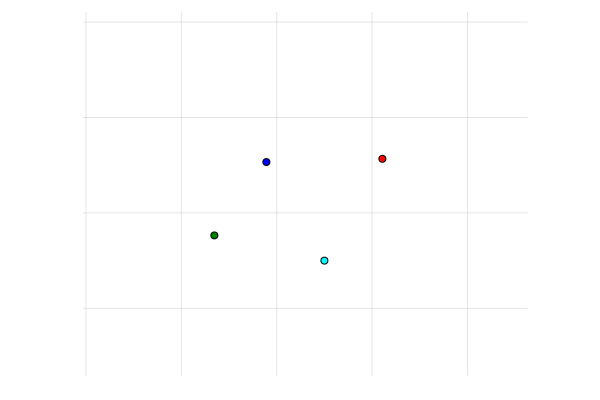
\includegraphics[width=.7\textwidth]{figures/mcd_instance.png}}
%		\source{Elaborated by the author.}
%		\label{fig:mcd_instance}
%	\end{figure}
%\end{frame}


\begin{frame}{Maximum Weight Clique Problem}{Algorithm}
	Defining $\Gamma_+(i,j)$ and $\Gamma_-(i,j)$:\\~\\

	Let $D_i$ (at the origin) and $D_j$ be two unit disks that have their corresponding circles intersect at two points.
	
	\begin{itemize}
		\item We know that the two intersection points define two arcs in $D_i$.
		\item One of the arcs bounds $D_i\cap D_j$. That is the one we want to determine.
		
		\item We can determine the polar angles of the two intersection points.
		%\item Assume $D_i$ is at the origin.
		\item Assuming counter-clockwise direction, we define $\Gamma_+(i,j)$ and $\Gamma_-(i,j)$ as the angles of intersection that determines the arc of $D_i$ that bounds $D_i \cap D_j$.
	\end{itemize}
\end{frame}

\begin{frame}{Maximum Weight Clique Problem}{Algorithm}

\begin{figure}
	\caption{$\Gamma_+(1,2)$ and $\Gamma_-(1,2)$ example.}
	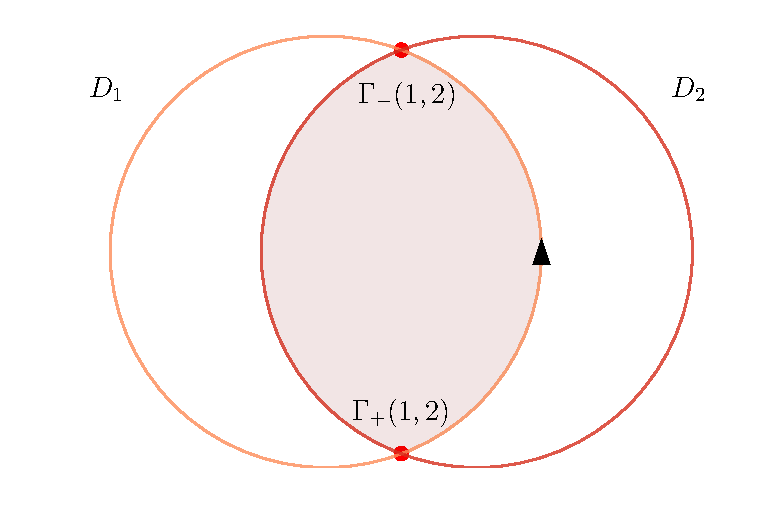
\includegraphics[scale=0.65]{figures/gammas.pdf}
		\source{Elaborated by the author.}
\end{figure}
\end{frame}

\begin{frame}{Maximum Weight Clique Problem}{Algorithm}
	\begin{figure}[H]
		\centering
		
		\caption{Three disks and their intersection points and angles.}
		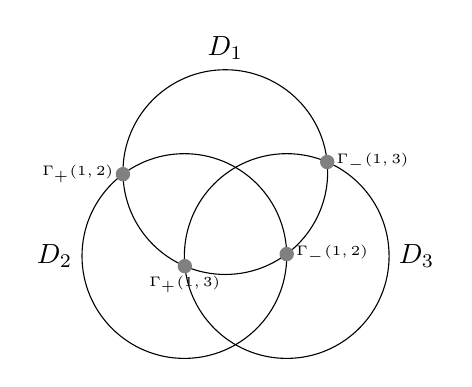
\begin{tikzpicture}[scale=1.3]
%\draw [help lines] (-5,-3) grid (5,3);

\draw[name path = c1] (0,0) circle (1cm);
\draw[name path = c3] (0.6,-0.82) circle (1cm);
\draw[name path = c2] (-0.4,-0.82) circle (1cm);

\node[above] at (0, 1) {$D_1$};
\node[left] at (-1.4, -0.82) {$D_2$};
\node[right] at (1.6, -0.82) {$D_3$};

\path [name intersections={of=c1 and c3}] ;
\foreach \i in {1,...,2}
\fill [color=gray] (intersection-\i) circle (2pt) ;

\node[right] at (intersection-1) {\tiny $\Gamma_-(1,3)$};
\node[left, below] at (intersection-2) {\tiny $\Gamma_+(1,3)$};

\path [name intersections={of=c1 and c2}] ;
\foreach \i in {1,...,2}
\fill [color=gray] (intersection-\i) circle (2pt) ;

\node[left] at (intersection-1) {\tiny $\Gamma_+(1,2)$};
\node[below,right] at (intersection-2) {\tiny $\Gamma_-(1,2)$};

%\draw [-] (-5,0) -- (5,0);
%\draw [-] (0,-3) -- (0,3);
%\draw [|-|] (0.001,-0.1) -- (4.999,-0.1);
\end{tikzpicture}
		\source{Elaborated by the author.}
		\label{fig:3disks_intersect}
	\end{figure}
\end{frame}


\begin{frame}{Maximum Weight Clique Problem}{Algorithm}
	
	Some observations allow us to arrive at the algorithm:
	
%	For a disk $D_i$, a counter-clockwise traversal visits every $\Gamma_+(i,j)$ and $\Gamma_-(i,j)$ in counter-clockwise order.
	
	\begin{itemize}
		\item An intersection region of disks is bounded by arcs.
		
		\item The arc $A(\Gamma_+(i,j),\Gamma_-(i,j))$ (counter-clockwise) determines a region where $i$ and $j$ intersect.
		

		\item For every disk $D_i$, we want to find an angle $\theta$, such that $$w(\{D_k : \theta \in A(\Gamma_+(i,k),\Gamma_-(i,k))\}),$$ is maximized. Most overlapping intervals (circular).
		
		\item To transform it to the problem of finding the most overlapping intervals, just copy the list of intersection angles. The arcs such that $\Gamma_+(i,j) > \Gamma_-(i,j)$ will be considered.
	\end{itemize}
\end{frame}

\begin{frame}{Maximum Weight Clique Problem}{Algorithm}
	
	Transforming it to the most overlapping intervals.
	
	\begin{figure}[H]
		\centering
		
		\caption{The intersections list of a disk with three other disks.}
		\tikzset{every picture/.style={line width=0.75pt}} %set default line width to 0.75pt        

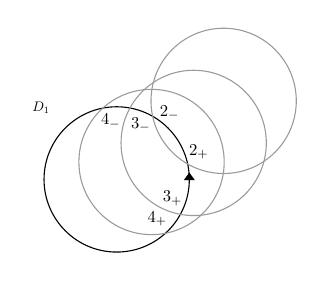
\begin{tikzpicture}[x=0.75pt,y=0.75pt,yscale=-1.4,xscale=1.4]
%uncomment if require: \path (0,95); %set diagram left start at 0, and has height of 95

%Shape: Circle [id:dp37777408295388804] 
\draw   (21,59.5) .. controls (21,45.69) and (32.19,34.5) .. (46,34.5) .. controls (59.81,34.5) and (71,45.69) .. (71,59.5) .. controls (71,73.31) and (59.81,84.5) .. (46,84.5) .. controls (32.19,84.5) and (21,73.31) .. (21,59.5) -- cycle ;
%Shape: Circle [id:dp4562198988843913] 
\draw  [color={rgb, 255:red, 155; green, 155; blue, 155 }  ,draw opacity=1 ] (47.5,46.94) .. controls (47.5,33.14) and (58.69,21.94) .. (72.5,21.94) .. controls (86.31,21.94) and (97.5,33.14) .. (97.5,46.94) .. controls (97.5,60.75) and (86.31,71.94) .. (72.5,71.94) .. controls (58.69,71.94) and (47.5,60.75) .. (47.5,46.94) -- cycle ;
%Shape: Circle [id:dp8913971633985722] 
\draw  [color={rgb, 255:red, 155; green, 155; blue, 155 }  ,draw opacity=1 ] (33,53.5) .. controls (33,39.69) and (44.19,28.5) .. (58,28.5) .. controls (71.81,28.5) and (83,39.69) .. (83,53.5) .. controls (83,67.31) and (71.81,78.5) .. (58,78.5) .. controls (44.19,78.5) and (33,67.31) .. (33,53.5) -- cycle ;
%Shape: Circle [id:dp05970043129919356] 
\draw  [color={rgb, 255:red, 155; green, 155; blue, 155 }  ,draw opacity=1 ] (57.81,32.47) .. controls (57.81,18.66) and (69,7.47) .. (82.81,7.47) .. controls (96.62,7.47) and (107.81,18.66) .. (107.81,32.47) .. controls (107.81,46.27) and (96.62,57.47) .. (82.81,57.47) .. controls (69,57.47) and (57.81,46.27) .. (57.81,32.47) -- cycle ;
%Straight Lines [id:da04725899028195979] 
%\draw[densely dotted]  (21,59.5) -- (71,59.5) ;


%Flowchart: Extract [id:dp5267407418119328] 
\draw  [fill={rgb, 255:red, 0; green, 0; blue, 0 }  ,fill opacity=1 ] (71,57.45) -- (72.52,59.55) -- (69.48,59.55) -- cycle ;

\draw (60,73) node [scale=0.6]  {$4_+$};
% Text Node
\draw (65.22,66) node [scale=0.6]  {$3_+$};
% Text Node
\draw (74.22,50) node [scale=0.6]  {$2_+$};
% Text Node
\draw (64.22,36.56) node [scale=0.6]  {$2_-$};
% Text Node
\draw (54.32,40.66) node [scale=0.6]  {$3_-$};
% Text Node
\draw (44.02,39.56) node [scale=0.6]  {$4_-$};


% Text Node
\draw (20,35) node [scale=0.5]  {$D_{1}$};
\end{tikzpicture}

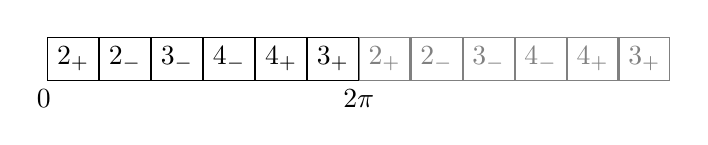
\begin{tikzpicture}

\matrix [matrix of nodes,row sep=,row sep=0mm,
column 1/.style={nodes={rectangle,draw,minimum width=1.5em, minimum height=0.5em}},
column 2/.style={nodes={rectangle,draw,minimum width=1.5em, minimum height=0.5em}},
column 3/.style={nodes={rectangle,draw,minimum width=1.5em, minimum height=0.5em}},
column 4/.style={nodes={rectangle,draw,minimum width=1.5em, minimum height=0.5em}},
column 5/.style={nodes={rectangle,draw,minimum width=1.5em, minimum height=0.5em}},
column 6/.style={nodes={rectangle,draw,minimum width=1.5em, minimum height=0.5em}},
column 7/.style={nodes={rectangle,draw,minimum width=1.5em, color=gray, minimum height=0.5em}},
column 8/.style={nodes={rectangle,draw,minimum width=1.5em, color=gray, minimum height=0.5em}},
column 9/.style={nodes={rectangle,draw,minimum width=1.5em, color=gray, minimum height=0.5em}},
column 10/.style={nodes={rectangle,draw,minimum width=1.5em, color=gray, minimum height=0.5em}},
column 11/.style={nodes={rectangle,draw,minimum width=1.5em, color=gray, minimum height=0.5em}},
column 12/.style={nodes={rectangle,draw,minimum width=1.5em, color=gray, minimum height=0.5em}}
] (O)
{
$2_+$ & $2_-$ & $3_-$ & $4_-$ & $4_+$ & $3_+$ & $2_+$ & $2_-$ & $3_-$ & $4_-$ & $4_+$ & $3_+$\\
%$+$ & $-$ & $-$ & $-$ & $+$ & $+$\\
};

\node at (-4,-0.5) {$0$};
\node at (0,-0.5) {$2\pi$};
\end{tikzpicture}
		\source{Elaborated by the author.}
		%\label{fig:array_disks}
	\end{figure}
\end{frame}

\begin{frame}{Maximum Weight Clique Problem}{Algorithm}
	Our algorithm for the Maximum Weight Clique Problem:\\~\\
	
	For every disk $D_i$, do:
	\begin{itemize}
		\item Get the sorted list of intersection angles with $D_i$
				$A=\cap_{j}\Gamma_+(i,j) \cup \Gamma_-(i,j)$.
		\item Traverse it twice starting at the angle with smallest value.
		\begin{itemize}
			\item Keep a set of active disks. When an opening angle is visited, make the disk active, otherwise remove it from the set.
			\item Update the optimal solution. Use the closing angle.
		\end{itemize}
	\end{itemize}
\end{frame}


%\begin{frame}{Maximum Weight Clique Problem}{Algorithm}
%\begin{figure}
	%\centering
	
%	\caption{A traversal for $D_1$ with green disks representing the active set and red signs representing the current angle being visited (some are omitted).}
%	\usetikzlibrary{matrix}



\tikzset{every picture/.style={line width=0.75pt}} %set default line width to 0.75pt        

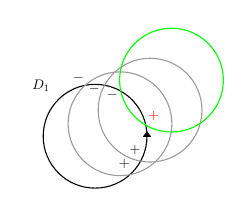
\begin{tikzpicture}[x=0.75pt,y=0.75pt,yscale=-1,xscale=1]
%uncomment if require: \path (0,95); %set diagram left start at 0, and has height of 95

%Shape: Circle [id:dp37777408295388804] 
\draw   (21,59.5) .. controls (21,45.69) and (32.19,34.5) .. (46,34.5) .. controls (59.81,34.5) and (71,45.69) .. (71,59.5) .. controls (71,73.31) and (59.81,84.5) .. (46,84.5) .. controls (32.19,84.5) and (21,73.31) .. (21,59.5) -- cycle ;
%Shape: Circle [id:dp4562198988843913] 
\draw  [color={rgb, 255:red, 155; green, 155; blue, 155 }  ,draw opacity=1 ] (47.5,46.94) .. controls (47.5,33.14) and (58.69,21.94) .. (72.5,21.94) .. controls (86.31,21.94) and (97.5,33.14) .. (97.5,46.94) .. controls (97.5,60.75) and (86.31,71.94) .. (72.5,71.94) .. controls (58.69,71.94) and (47.5,60.75) .. (47.5,46.94) -- cycle ;
%Shape: Circle [id:dp8913971633985722] 
\draw  [color={rgb, 255:red, 155; green, 155; blue, 155 }  ,draw opacity=1 ] (33,53.5) .. controls (33,39.69) and (44.19,28.5) .. (58,28.5) .. controls (71.81,28.5) and (83,39.69) .. (83,53.5) .. controls (83,67.31) and (71.81,78.5) .. (58,78.5) .. controls (44.19,78.5) and (33,67.31) .. (33,53.5) -- cycle ;
%Shape: Circle [id:dp05970043129919356] 
\draw  [color=green  ,draw opacity=1 ] (57.81,32.47) .. controls (57.81,18.66) and (69,7.47) .. (82.81,7.47) .. controls (96.62,7.47) and (107.81,18.66) .. (107.81,32.47) .. controls (107.81,46.27) and (96.62,57.47) .. (82.81,57.47) .. controls (69,57.47) and (57.81,46.27) .. (57.81,32.47) -- cycle ;
%Straight Lines [id:da04725899028195979] 
%\draw[densely dotted]  (21,59.5) -- (71,59.5) ;


%Flowchart: Extract [id:dp5267407418119328] 
\draw  [fill={rgb, 255:red, 0; green, 0; blue, 0 }  ,fill opacity=1 ] (71,57.45) -- (72.52,59.55) -- (69.48,59.55) -- cycle ;

\draw (60,73) node [scale=0.5]  {$+$};
% Text Node
\draw (65.22,66) node [scale=0.5]  {$+$};
% Text Node
\draw (74.22,50) node [scale=0.5,color=red]  {$+$};
% Text Node
\draw (54.22,39.56) node [scale=0.5]  {$-$};
% Text Node
\draw (45.62,36.96) node [scale=0.5]  {$-$};
% Text Node
\draw (38.02,31.56) node [scale=0.5]  {$-$};


% Text Node
\draw (20,35) node [scale=0.5]  {$D_{1}$};
\end{tikzpicture}
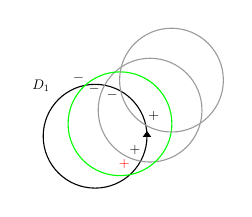
\begin{tikzpicture}[x=0.75pt,y=0.75pt,yscale=-1,xscale=1]
%uncomment if require: \path (0,95); %set diagram left start at 0, and has height of 95

%Shape: Circle [id:dp37777408295388804] 
\draw   (21,59.5) .. controls (21,45.69) and (32.19,34.5) .. (46,34.5) .. controls (59.81,34.5) and (71,45.69) .. (71,59.5) .. controls (71,73.31) and (59.81,84.5) .. (46,84.5) .. controls (32.19,84.5) and (21,73.31) .. (21,59.5) -- cycle ;
%Shape: Circle [id:dp4562198988843913] 
\draw  [color={rgb, 255:red, 155; green, 155; blue, 155 }  ,draw opacity=1 ] (47.5,46.94) .. controls (47.5,33.14) and (58.69,21.94) .. (72.5,21.94) .. controls (86.31,21.94) and (97.5,33.14) .. (97.5,46.94) .. controls (97.5,60.75) and (86.31,71.94) .. (72.5,71.94) .. controls (58.69,71.94) and (47.5,60.75) .. (47.5,46.94) -- cycle ;
%Shape: Circle [id:dp8913971633985722] 
\draw  [color=green  ,draw opacity=1 ] (33,53.5) .. controls (33,39.69) and (44.19,28.5) .. (58,28.5) .. controls (71.81,28.5) and (83,39.69) .. (83,53.5) .. controls (83,67.31) and (71.81,78.5) .. (58,78.5) .. controls (44.19,78.5) and (33,67.31) .. (33,53.5) -- cycle ;
%Shape: Circle [id:dp05970043129919356] 
\draw  [color={rgb, 255:red, 155; green, 155; blue, 155 }  ,draw opacity=1 ] (57.81,32.47) .. controls (57.81,18.66) and (69,7.47) .. (82.81,7.47) .. controls (96.62,7.47) and (107.81,18.66) .. (107.81,32.47) .. controls (107.81,46.27) and (96.62,57.47) .. (82.81,57.47) .. controls (69,57.47) and (57.81,46.27) .. (57.81,32.47) -- cycle ;
%Straight Lines [id:da04725899028195979] 
%\draw[densely dotted]  (21,59.5) -- (71,59.5) ;


%Flowchart: Extract [id:dp5267407418119328] 
\draw  [fill={rgb, 255:red, 0; green, 0; blue, 0 }  ,fill opacity=1 ] (71,57.45) -- (72.52,59.55) -- (69.48,59.55) -- cycle ;

\draw (60,73) node [scale=0.5,color=red]  {$+$};
% Text Node
\draw (65.22,66) node [scale=0.5]  {$+$};
% Text Node
\draw (74.22,50) node [scale=0.5]  {$+$};
% Text Node
\draw (54.22,39.56) node [scale=0.5]  {$-$};
% Text Node
\draw (45.62,36.96) node [scale=0.5]  {$-$};
% Text Node
\draw (38.02,31.56) node [scale=0.5]  {$-$};


% Text Node
\draw (20,35) node [scale=0.5]  {$D_{1}$};
\end{tikzpicture}
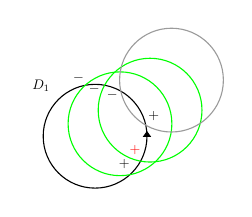
\begin{tikzpicture}[x=0.75pt,y=0.75pt,yscale=-1,xscale=1]
%uncomment if require: \path (0,95); %set diagram left start at 0, and has height of 95

%Shape: Circle [id:dp37777408295388804] 
\draw   (21,59.5) .. controls (21,45.69) and (32.19,34.5) .. (46,34.5) .. controls (59.81,34.5) and (71,45.69) .. (71,59.5) .. controls (71,73.31) and (59.81,84.5) .. (46,84.5) .. controls (32.19,84.5) and (21,73.31) .. (21,59.5) -- cycle ;


%Shape: Circle [id:dp4562198988843913] 
\draw  [color=green  ,draw opacity=1 ] (47.5,46.94) .. controls (47.5,33.14) and (58.69,21.94) .. (72.5,21.94) .. controls (86.31,21.94) and (97.5,33.14) .. (97.5,46.94) .. controls (97.5,60.75) and (86.31,71.94) .. (72.5,71.94) .. controls (58.69,71.94) and (47.5,60.75) .. (47.5,46.94) -- cycle ;


%Shape: Circle [id:dp8913971633985722] 
\draw  [color=green  ,draw opacity=1 ] (33,53.5) .. controls (33,39.69) and (44.19,28.5) .. (58,28.5) .. controls (71.81,28.5) and (83,39.69) .. (83,53.5) .. controls (83,67.31) and (71.81,78.5) .. (58,78.5) .. controls (44.19,78.5) and (33,67.31) .. (33,53.5) -- cycle ;


%Shape: Circle [id:dp05970043129919356] 
\draw  [color={rgb, 255:red, 155; green, 155; blue, 155 }  ,draw opacity=1 ] (57.81,32.47) .. controls (57.81,18.66) and (69,7.47) .. (82.81,7.47) .. controls (96.62,7.47) and (107.81,18.66) .. (107.81,32.47) .. controls (107.81,46.27) and (96.62,57.47) .. (82.81,57.47) .. controls (69,57.47) and (57.81,46.27) .. (57.81,32.47) -- cycle ;
%Straight Lines [id:da04725899028195979] 
%\draw[densely dotted]  (21,59.5) -- (71,59.5) ;


%Flowchart: Extract [id:dp5267407418119328] 
\draw  [fill={rgb, 255:red, 0; green, 0; blue, 0 }  ,fill opacity=1 ] (71,57.45) -- (72.52,59.55) -- (69.48,59.55) -- cycle ;

\draw (60,73) node [scale=0.5]  {$+$};
% Text Node
\draw (65.22,66) node [scale=0.5,color=red]  {$+$};
% Text Node
\draw (74.22,50) node [scale=0.5]  {$+$};
% Text Node
\draw (54.22,39.56) node [scale=0.5]  {$-$};
% Text Node
\draw (45.62,36.96) node [scale=0.5]  {$-$};
% Text Node
\draw (38.02,31.56) node [scale=0.5]  {$-$};


% Text Node
\draw (20,35) node [scale=0.5]  {$D_{1}$};
\end{tikzpicture}
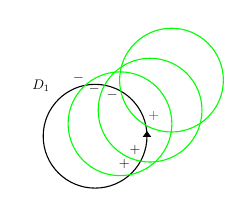
\begin{tikzpicture}[x=0.75pt,y=0.75pt,yscale=-1,xscale=1]
%uncomment if require: \path (0,95); %set diagram left start at 0, and has height of 95

%Shape: Circle [id:dp37777408295388804] 
\draw   (21,59.5) .. controls (21,45.69) and (32.19,34.5) .. (46,34.5) .. controls (59.81,34.5) and (71,45.69) .. (71,59.5) .. controls (71,73.31) and (59.81,84.5) .. (46,84.5) .. controls (32.19,84.5) and (21,73.31) .. (21,59.5) -- cycle ;


%Shape: Circle [id:dp4562198988843913] 
\draw  [color=green  ,draw opacity=1 ] (47.5,46.94) .. controls (47.5,33.14) and (58.69,21.94) .. (72.5,21.94) .. controls (86.31,21.94) and (97.5,33.14) .. (97.5,46.94) .. controls (97.5,60.75) and (86.31,71.94) .. (72.5,71.94) .. controls (58.69,71.94) and (47.5,60.75) .. (47.5,46.94) -- cycle ;


%Shape: Circle [id:dp8913971633985722] 
\draw  [color=green  ,draw opacity=1 ] (33,53.5) .. controls (33,39.69) and (44.19,28.5) .. (58,28.5) .. controls (71.81,28.5) and (83,39.69) .. (83,53.5) .. controls (83,67.31) and (71.81,78.5) .. (58,78.5) .. controls (44.19,78.5) and (33,67.31) .. (33,53.5) -- cycle ;


%Shape: Circle [id:dp05970043129919356] 
\draw  [color=green ,draw opacity=1 ] (57.81,32.47) .. controls (57.81,18.66) and (69,7.47) .. (82.81,7.47) .. controls (96.62,7.47) and (107.81,18.66) .. (107.81,32.47) .. controls (107.81,46.27) and (96.62,57.47) .. (82.81,57.47) .. controls (69,57.47) and (57.81,46.27) .. (57.81,32.47) -- cycle ;
%Straight Lines [id:da04725899028195979] 
%\draw[densely dotted]  (21,59.5) -- (71,59.5) ;


%Flowchart: Extract [id:dp5267407418119328] 
\draw  [fill={rgb, 255:red, 0; green, 0; blue, 0 }  ,fill opacity=1 ] (71,57.45) -- (72.52,59.55) -- (69.48,59.55) -- cycle ;

\draw (60,73) node [scale=0.5]  {$+$};
% Text Node
\draw (65.22,66) node [scale=0.5]  {$+$};
% Text Node
\draw (74.22,50) node [scale=0.5,color=red]  {$+$};
% Text Node
\draw (54.22,39.56) node [scale=0.5]  {$-$};
% Text Node
\draw (45.62,36.96) node [scale=0.5]  {$-$};
% Text Node
\draw (38.02,31.56) node [scale=0.5]  {$-$};


% Text Node
\draw (20,35) node [scale=0.5]  {$D_{1}$};
\end{tikzpicture}
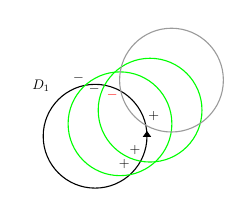
\begin{tikzpicture}[x=0.75pt,y=0.75pt,yscale=-1,xscale=1]
%uncomment if require: \path (0,95); %set diagram left start at 0, and has height of 95

%Shape: Circle [id:dp37777408295388804] 
\draw   (21,59.5) .. controls (21,45.69) and (32.19,34.5) .. (46,34.5) .. controls (59.81,34.5) and (71,45.69) .. (71,59.5) .. controls (71,73.31) and (59.81,84.5) .. (46,84.5) .. controls (32.19,84.5) and (21,73.31) .. (21,59.5) -- cycle ;


%Shape: Circle [id:dp4562198988843913] 
\draw  [color=green  ,draw opacity=1 ] (47.5,46.94) .. controls (47.5,33.14) and (58.69,21.94) .. (72.5,21.94) .. controls (86.31,21.94) and (97.5,33.14) .. (97.5,46.94) .. controls (97.5,60.75) and (86.31,71.94) .. (72.5,71.94) .. controls (58.69,71.94) and (47.5,60.75) .. (47.5,46.94) -- cycle ;


%Shape: Circle [id:dp8913971633985722] 
\draw  [color=green  ,draw opacity=1 ] (33,53.5) .. controls (33,39.69) and (44.19,28.5) .. (58,28.5) .. controls (71.81,28.5) and (83,39.69) .. (83,53.5) .. controls (83,67.31) and (71.81,78.5) .. (58,78.5) .. controls (44.19,78.5) and (33,67.31) .. (33,53.5) -- cycle ;


%Shape: Circle [id:dp05970043129919356] 
\draw  [color={rgb, 255:red, 155; green, 155; blue, 155 }  ,draw opacity=1 ] (57.81,32.47) .. controls (57.81,18.66) and (69,7.47) .. (82.81,7.47) .. controls (96.62,7.47) and (107.81,18.66) .. (107.81,32.47) .. controls (107.81,46.27) and (96.62,57.47) .. (82.81,57.47) .. controls (69,57.47) and (57.81,46.27) .. (57.81,32.47) -- cycle ;
%Straight Lines [id:da04725899028195979] 
%\draw[densely dotted]  (21,59.5) -- (71,59.5) ;


%Flowchart: Extract [id:dp5267407418119328] 
\draw  [fill={rgb, 255:red, 0; green, 0; blue, 0 }  ,fill opacity=1 ] (71,57.45) -- (72.52,59.55) -- (69.48,59.55) -- cycle ;

\draw (60,73) node [scale=0.5]  {$+$};
% Text Node
\draw (65.22,66) node [scale=0.5]  {$+$};
% Text Node
\draw (74.22,50) node [scale=0.5]  {$+$};
% Text Node
\draw (54.22,39.56) node [scale=0.5,color=red]  {$-$};
% Text Node
\draw (45.62,36.96) node [scale=0.5]  {$-$};
% Text Node
\draw (38.02,31.56) node [scale=0.5]  {$-$};


% Text Node
\draw (20,35) node [scale=0.5]  {$D_{1}$};
\end{tikzpicture}
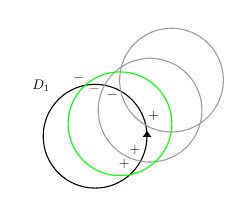
\begin{tikzpicture}[x=0.75pt,y=0.75pt,yscale=-1,xscale=1]
%uncomment if require: \path (0,95); %set diagram left start at 0, and has height of 95

%Shape: Circle [id:dp37777408295388804] 
\draw   (21,59.5) .. controls (21,45.69) and (32.19,34.5) .. (46,34.5) .. controls (59.81,34.5) and (71,45.69) .. (71,59.5) .. controls (71,73.31) and (59.81,84.5) .. (46,84.5) .. controls (32.19,84.5) and (21,73.31) .. (21,59.5) -- cycle ;


%Shape: Circle [id:dp4562198988843913] 
\draw  [color={rgb, 255:red, 155; green, 155; blue, 155 },draw opacity=1 ] (47.5,46.94) .. controls (47.5,33.14) and (58.69,21.94) .. (72.5,21.94) .. controls (86.31,21.94) and (97.5,33.14) .. (97.5,46.94) .. controls (97.5,60.75) and (86.31,71.94) .. (72.5,71.94) .. controls (58.69,71.94) and (47.5,60.75) .. (47.5,46.94) -- cycle ;


%Shape: Circle [id:dp8913971633985722] 
\draw  [color=green  ,draw opacity=1 ] (33,53.5) .. controls (33,39.69) and (44.19,28.5) .. (58,28.5) .. controls (71.81,28.5) and (83,39.69) .. (83,53.5) .. controls (83,67.31) and (71.81,78.5) .. (58,78.5) .. controls (44.19,78.5) and (33,67.31) .. (33,53.5) -- cycle ;


%Shape: Circle [id:dp05970043129919356] 
\draw  [color={rgb, 255:red, 155; green, 155; blue, 155 }  ,draw opacity=1 ] (57.81,32.47) .. controls (57.81,18.66) and (69,7.47) .. (82.81,7.47) .. controls (96.62,7.47) and (107.81,18.66) .. (107.81,32.47) .. controls (107.81,46.27) and (96.62,57.47) .. (82.81,57.47) .. controls (69,57.47) and (57.81,46.27) .. (57.81,32.47) -- cycle ;
%Straight Lines [id:da04725899028195979] 
%\draw[densely dotted]  (21,59.5) -- (71,59.5) ;


%Flowchart: Extract [id:dp5267407418119328] 
\draw  [fill={rgb, 255:red, 0; green, 0; blue, 0 }  ,fill opacity=1 ] (71,57.45) -- (72.52,59.55) -- (69.48,59.55) -- cycle ;

\draw (60,73) node [scale=0.5]  {$+$};
% Text Node
\draw (65.22,66) node [scale=0.5]  {$+$};
% Text Node
\draw (74.22,50) node [scale=0.5]  {$+$};
% Text Node
\draw (54.22,39.56) node [scale=0.5]  {$-$};
% Text Node
\draw (45.62,36.96) node [scale=0.5,color=red]  {$-$};
% Text Node
\draw (38.02,31.56) node [scale=0.5]  {$-$};


% Text Node
\draw (20,35) node [scale=0.5]  {$D_{1}$};
\end{tikzpicture}
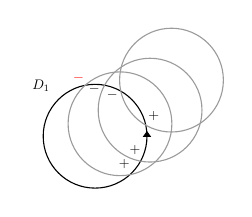
\begin{tikzpicture}[x=0.75pt,y=0.75pt,yscale=-1,xscale=1]
%uncomment if require: \path (0,95); %set diagram left start at 0, and has height of 95

%Shape: Circle [id:dp37777408295388804] 
\draw   (21,59.5) .. controls (21,45.69) and (32.19,34.5) .. (46,34.5) .. controls (59.81,34.5) and (71,45.69) .. (71,59.5) .. controls (71,73.31) and (59.81,84.5) .. (46,84.5) .. controls (32.19,84.5) and (21,73.31) .. (21,59.5) -- cycle ;


%Shape: Circle [id:dp4562198988843913] 
\draw  [color={rgb, 255:red, 155; green, 155; blue, 155 },draw opacity=1 ] (47.5,46.94) .. controls (47.5,33.14) and (58.69,21.94) .. (72.5,21.94) .. controls (86.31,21.94) and (97.5,33.14) .. (97.5,46.94) .. controls (97.5,60.75) and (86.31,71.94) .. (72.5,71.94) .. controls (58.69,71.94) and (47.5,60.75) .. (47.5,46.94) -- cycle ;


%Shape: Circle [id:dp8913971633985722] 
\draw  [color={rgb, 255:red, 155; green, 155; blue, 155 } ,draw opacity=1 ] (33,53.5) .. controls (33,39.69) and (44.19,28.5) .. (58,28.5) .. controls (71.81,28.5) and (83,39.69) .. (83,53.5) .. controls (83,67.31) and (71.81,78.5) .. (58,78.5) .. controls (44.19,78.5) and (33,67.31) .. (33,53.5) -- cycle ;


%Shape: Circle [id:dp05970043129919356] 
\draw  [color={rgb, 255:red, 155; green, 155; blue, 155 }  ,draw opacity=1 ] (57.81,32.47) .. controls (57.81,18.66) and (69,7.47) .. (82.81,7.47) .. controls (96.62,7.47) and (107.81,18.66) .. (107.81,32.47) .. controls (107.81,46.27) and (96.62,57.47) .. (82.81,57.47) .. controls (69,57.47) and (57.81,46.27) .. (57.81,32.47) -- cycle ;
%Straight Lines [id:da04725899028195979] 
%\draw[densely dotted]  (21,59.5) -- (71,59.5) ;


%Flowchart: Extract [id:dp5267407418119328] 
\draw  [fill={rgb, 255:red, 0; green, 0; blue, 0 }  ,fill opacity=1 ] (71,57.45) -- (72.52,59.55) -- (69.48,59.55) -- cycle ;

\draw (60,73) node [scale=0.5]  {$+$};
% Text Node
\draw (65.22,66) node [scale=0.5]  {$+$};
% Text Node
\draw (74.22,50) node [scale=0.5]  {$+$};
% Text Node
\draw (54.22,39.56) node [scale=0.5]  {$-$};
% Text Node
\draw (45.62,36.96) node [scale=0.5]  {$-$};
% Text Node
\draw (38.02,31.56) node [scale=0.5,color=red]  {\textbf{$-$}};


% Text Node
\draw (20,35) node [scale=0.5]  {$D_{1}$};
\end{tikzpicture}



%		\source{Elaborated by the author.}
	%\label{fig:array_disks}
%\end{figure}
%\end{frame}

\begin{frame}{Maximum Weight Clique Problem}{Algorithm}

	\begin{figure}
		\caption{A traversal for $D_1$ with green disks representing the active set and red signs representing the current angle being visited (some are omitted).}
		\only<1>{\tikzset{every picture/.style={line width=0.75pt}} %set default line width to 0.75pt        

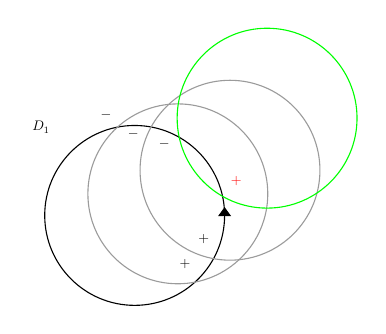
\begin{tikzpicture}[x=1pt,y=1pt,yscale=-1.3,xscale=1.3]
%uncomment if require: \path (0,95); %set diagram left start at 0, and has height of 95

%Shape: Circle [id:dp37777408295388804] 
\draw   (21,59.5) .. controls (21,45.69) and (32.19,34.5) .. (46,34.5) .. controls (59.81,34.5) and (71,45.69) .. (71,59.5) .. controls (71,73.31) and (59.81,84.5) .. (46,84.5) .. controls (32.19,84.5) and (21,73.31) .. (21,59.5) -- cycle ;
%Shape: Circle [id:dp4562198988843913] 
\draw  [color={rgb, 255:red, 155; green, 155; blue, 155 }  ,draw opacity=1 ] (47.5,46.94) .. controls (47.5,33.14) and (58.69,21.94) .. (72.5,21.94) .. controls (86.31,21.94) and (97.5,33.14) .. (97.5,46.94) .. controls (97.5,60.75) and (86.31,71.94) .. (72.5,71.94) .. controls (58.69,71.94) and (47.5,60.75) .. (47.5,46.94) -- cycle ;
%Shape: Circle [id:dp8913971633985722] 
\draw  [color={rgb, 255:red, 155; green, 155; blue, 155 }  ,draw opacity=1 ] (33,53.5) .. controls (33,39.69) and (44.19,28.5) .. (58,28.5) .. controls (71.81,28.5) and (83,39.69) .. (83,53.5) .. controls (83,67.31) and (71.81,78.5) .. (58,78.5) .. controls (44.19,78.5) and (33,67.31) .. (33,53.5) -- cycle ;
%Shape: Circle [id:dp05970043129919356] 
\draw  [color=green  ,draw opacity=1 ] (57.81,32.47) .. controls (57.81,18.66) and (69,7.47) .. (82.81,7.47) .. controls (96.62,7.47) and (107.81,18.66) .. (107.81,32.47) .. controls (107.81,46.27) and (96.62,57.47) .. (82.81,57.47) .. controls (69,57.47) and (57.81,46.27) .. (57.81,32.47) -- cycle ;
%Straight Lines [id:da04725899028195979] 
%\draw[densely dotted]  (21,59.5) -- (71,59.5) ;


%Flowchart: Extract [id:dp5267407418119328] 
\draw  [fill={rgb, 255:red, 0; green, 0; blue, 0 }  ,fill opacity=1 ] (71,57.45) -- (72.52,59.55) -- (69.48,59.55) -- cycle ;

\draw (60,73) node [scale=0.5]  {$+$};
% Text Node
\draw (65.22,66) node [scale=0.5]  {$+$};
% Text Node
\draw (74.22,50) node [scale=0.5,color=red]  {$+$};
% Text Node
\draw (54.22,39.56) node [scale=0.5]  {$-$};
% Text Node
\draw (45.62,36.96) node [scale=0.5]  {$-$};
% Text Node
\draw (38.02,31.56) node [scale=0.5]  {$-$};


% Text Node
\draw (20,35) node [scale=0.5]  {$D_{1}$};
\end{tikzpicture}

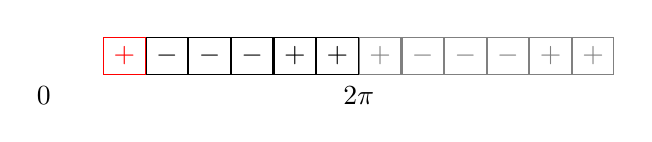
\begin{tikzpicture}

\matrix [matrix of nodes,row sep=,row sep=0mm,
column 1/.style={nodes={rectangle,draw,minimum width=1.5em, color=red,minimum height=0.5em}},
column 2/.style={nodes={rectangle,draw,minimum width=1.5em, minimum height=0.5em}},
column 3/.style={nodes={rectangle,draw,minimum width=1.5em, minimum height=0.5em}},
column 4/.style={nodes={rectangle,draw,minimum width=1.5em, minimum height=0.5em}},
column 5/.style={nodes={rectangle,draw,minimum width=1.5em, minimum height=0.5em}},
column 6/.style={nodes={rectangle,draw,minimum width=1.5em, minimum height=0.5em}},
column 7/.style={nodes={rectangle,draw,minimum width=1.5em, color=gray, minimum height=0.5em}},
column 8/.style={nodes={rectangle,draw,minimum width=1.5em, color=gray, minimum height=0.5em}},
column 9/.style={nodes={rectangle,draw,minimum width=1.5em, color=gray, minimum height=0.5em}},
column 10/.style={nodes={rectangle,draw,minimum width=1.5em, color=gray, minimum height=0.5em}},
column 11/.style={nodes={rectangle,draw,minimum width=1.5em, color=gray, minimum height=0.5em}},
column 12/.style={nodes={rectangle,draw,minimum width=1.5em, color=gray, minimum height=0.5em}}
] (O)
{
	$+$ & $-$ & $-$ & $-$ & $+$ & $+$ & $+$ & $-$ & $-$ & $-$ & $+$ & $+$\\
	%$+$ & $-$ & $-$ & $-$ & $+$ & $+$\\
};

\node at (-4,-0.5) {$0$};
\node at (0,-0.5) {$2\pi$};
\end{tikzpicture}}
		\only<2>{\tikzset{every picture/.style={line width=0.75pt}} %set default line width to 0.75pt        

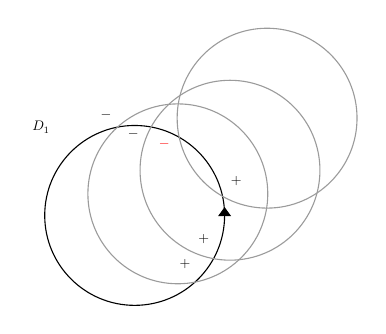
\begin{tikzpicture}[x=1pt,y=1pt,yscale=-1.3,xscale=1.3]
%uncomment if require: \path (0,95); %set diagram left start at 0, and has height of 95

%Shape: Circle [id:dp37777408295388804] 
\draw   (21,59.5) .. controls (21,45.69) and (32.19,34.5) .. (46,34.5) .. controls (59.81,34.5) and (71,45.69) .. (71,59.5) .. controls (71,73.31) and (59.81,84.5) .. (46,84.5) .. controls (32.19,84.5) and (21,73.31) .. (21,59.5) -- cycle ;
%Shape: Circle [id:dp4562198988843913] 
\draw  [color={rgb, 255:red, 155; green, 155; blue, 155 }  ,draw opacity=1 ] (47.5,46.94) .. controls (47.5,33.14) and (58.69,21.94) .. (72.5,21.94) .. controls (86.31,21.94) and (97.5,33.14) .. (97.5,46.94) .. controls (97.5,60.75) and (86.31,71.94) .. (72.5,71.94) .. controls (58.69,71.94) and (47.5,60.75) .. (47.5,46.94) -- cycle ;
%Shape: Circle [id:dp8913971633985722] 
\draw  [color={rgb, 255:red, 155; green, 155; blue, 155 }  ,draw opacity=1 ] (33,53.5) .. controls (33,39.69) and (44.19,28.5) .. (58,28.5) .. controls (71.81,28.5) and (83,39.69) .. (83,53.5) .. controls (83,67.31) and (71.81,78.5) .. (58,78.5) .. controls (44.19,78.5) and (33,67.31) .. (33,53.5) -- cycle ;
%Shape: Circle [id:dp05970043129919356] 
\draw  [color={rgb, 255:red, 155; green, 155; blue, 155 } ,draw opacity=1 ] (57.81,32.47) .. controls (57.81,18.66) and (69,7.47) .. (82.81,7.47) .. controls (96.62,7.47) and (107.81,18.66) .. (107.81,32.47) .. controls (107.81,46.27) and (96.62,57.47) .. (82.81,57.47) .. controls (69,57.47) and (57.81,46.27) .. (57.81,32.47) -- cycle ;
%Straight Lines [id:da04725899028195979] 
%\draw[densely dotted]  (21,59.5) -- (71,59.5) ;


%Flowchart: Extract [id:dp5267407418119328] 
\draw  [fill={rgb, 255:red, 0; green, 0; blue, 0 }  ,fill opacity=1 ] (71,57.45) -- (72.52,59.55) -- (69.48,59.55) -- cycle ;

\draw (60,73) node [scale=0.5]  {$+$};
% Text Node
\draw (65.22,66) node [scale=0.5]  {$+$};
% Text Node
\draw (74.22,50) node [scale=0.5]  {$+$};
% Text Node
\draw (54.22,39.56) node [scale=0.5,color=red]  {$-$};
% Text Node
\draw (45.62,36.96) node [scale=0.5]  {$-$};
% Text Node
\draw (38.02,31.56) node [scale=0.5]  {$-$};


% Text Node
\draw (20,35) node [scale=0.5]  {$D_{1}$};
\end{tikzpicture}

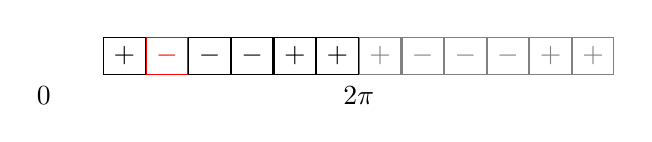
\begin{tikzpicture}

\matrix [matrix of nodes,row sep=,row sep=0mm,
column 1/.style={nodes={rectangle,draw,minimum width=1.5em, minimum height=0.5em}},
column 2/.style={nodes={rectangle,draw,minimum width=1.5em, color=red,minimum height=0.5em}},
column 3/.style={nodes={rectangle,draw,minimum width=1.5em, minimum height=0.5em}},
column 4/.style={nodes={rectangle,draw,minimum width=1.5em, minimum height=0.5em}},
column 5/.style={nodes={rectangle,draw,minimum width=1.5em, minimum height=0.5em}},
column 6/.style={nodes={rectangle,draw,minimum width=1.5em, minimum height=0.5em}},
column 7/.style={nodes={rectangle,draw,minimum width=1.5em, color=gray, minimum height=0.5em}},
column 8/.style={nodes={rectangle,draw,minimum width=1.5em, color=gray, minimum height=0.5em}},
column 9/.style={nodes={rectangle,draw,minimum width=1.5em, color=gray, minimum height=0.5em}},
column 10/.style={nodes={rectangle,draw,minimum width=1.5em, color=gray, minimum height=0.5em}},
column 11/.style={nodes={rectangle,draw,minimum width=1.5em, color=gray, minimum height=0.5em}},
column 12/.style={nodes={rectangle,draw,minimum width=1.5em, color=gray, minimum height=0.5em}}
] (O)
{
	$+$ & $-$ & $-$ & $-$ & $+$ & $+$ & $+$ & $-$ & $-$ & $-$ & $+$ & $+$\\
	%$+$ & $-$ & $-$ & $-$ & $+$ & $+$\\
};

\node at (-4,-0.5) {$0$};
\node at (0,-0.5) {$2\pi$};
\end{tikzpicture}}
		\only<3>{\tikzset{every picture/.style={line width=0.75pt}} %set default line width to 0.75pt        

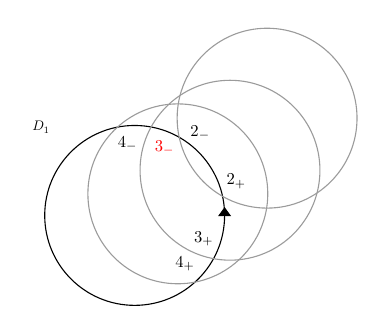
\begin{tikzpicture}[x=1pt,y=1pt,yscale=-1.3,xscale=1.3]
%uncomment if require: \path (0,95); %set diagram left start at 0, and has height of 95

%Shape: Circle [id:dp37777408295388804] 
\draw   (21,59.5) .. controls (21,45.69) and (32.19,34.5) .. (46,34.5) .. controls (59.81,34.5) and (71,45.69) .. (71,59.5) .. controls (71,73.31) and (59.81,84.5) .. (46,84.5) .. controls (32.19,84.5) and (21,73.31) .. (21,59.5) -- cycle ;
%Shape: Circle [id:dp4562198988843913] 
\draw  [color={rgb, 255:red, 155; green, 155; blue, 155 }  ,draw opacity=1 ] (47.5,46.94) .. controls (47.5,33.14) and (58.69,21.94) .. (72.5,21.94) .. controls (86.31,21.94) and (97.5,33.14) .. (97.5,46.94) .. controls (97.5,60.75) and (86.31,71.94) .. (72.5,71.94) .. controls (58.69,71.94) and (47.5,60.75) .. (47.5,46.94) -- cycle ;
%Shape: Circle [id:dp8913971633985722] 
\draw  [color={rgb, 255:red, 155; green, 155; blue, 155 }  ,draw opacity=1 ] (33,53.5) .. controls (33,39.69) and (44.19,28.5) .. (58,28.5) .. controls (71.81,28.5) and (83,39.69) .. (83,53.5) .. controls (83,67.31) and (71.81,78.5) .. (58,78.5) .. controls (44.19,78.5) and (33,67.31) .. (33,53.5) -- cycle ;
%Shape: Circle [id:dp05970043129919356] 
\draw  [color={rgb, 255:red, 155; green, 155; blue, 155 } ,draw opacity=1 ] (57.81,32.47) .. controls (57.81,18.66) and (69,7.47) .. (82.81,7.47) .. controls (96.62,7.47) and (107.81,18.66) .. (107.81,32.47) .. controls (107.81,46.27) and (96.62,57.47) .. (82.81,57.47) .. controls (69,57.47) and (57.81,46.27) .. (57.81,32.47) -- cycle ;
%Straight Lines [id:da04725899028195979] 
%\draw[densely dotted]  (21,59.5) -- (71,59.5) ;


%Flowchart: Extract [id:dp5267407418119328] 
\draw  [fill={rgb, 255:red, 0; green, 0; blue, 0 }  ,fill opacity=1 ] (71,57.45) -- (72.52,59.55) -- (69.48,59.55) -- cycle ;

\draw (60,73) node [scale=0.6]  {$4_+$};
% Text Node
\draw (65.22,66) node [scale=0.6]  {$3_+$};
% Text Node
\draw (74.22,50) node [scale=0.6]  {$2_+$};
% Text Node
\draw (64.22,36.56) node [scale=0.6]  {$2_-$};
% Text Node
\draw (54.32,40.66) node [scale=0.6,color=red]  {$3_-$};
% Text Node
\draw (44.02,39.56) node [scale=0.6]  {$4_-$};

% Text Node
\draw (20,35) node [scale=0.5]  {$D_{1}$};
\end{tikzpicture}

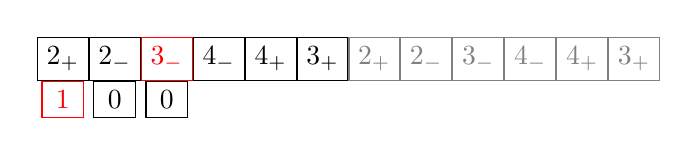
\begin{tikzpicture}

\matrix [matrix of nodes,row sep=,row sep=0mm,
column 1/.style={nodes={rectangle,draw,minimum width=1.5em, minimum height=0.5em}},
column 2/.style={nodes={rectangle,draw,minimum width=1.5em, minimum height=0.5em}},
column 3/.style={nodes={rectangle,draw,minimum width=1.5em, color=red, minimum height=0.5em}},
column 4/.style={nodes={rectangle,draw,minimum width=1.5em, minimum height=0.5em}},
column 5/.style={nodes={rectangle,draw,minimum width=1.5em, minimum height=0.5em}},
column 6/.style={nodes={rectangle,draw,minimum width=1.5em, minimum height=0.5em}},
column 7/.style={nodes={rectangle,draw,minimum width=1.5em, color=gray, minimum height=0.5em}},
column 8/.style={nodes={rectangle,draw,minimum width=1.5em, color=gray, minimum height=0.5em}},
column 9/.style={nodes={rectangle,draw,minimum width=1.5em, color=gray, minimum height=0.5em}},
column 10/.style={nodes={rectangle,draw,minimum width=1.5em, color=gray, minimum height=0.5em}},
column 11/.style={nodes={rectangle,draw,minimum width=1.5em, color=gray, minimum height=0.5em}},
column 12/.style={nodes={rectangle,draw,minimum width=1.5em, color=gray, minimum height=0.5em}}
] (O)
{
$2_+$ & $2_-$ & $3_-$ & $4_-$ & $4_+$ & $3_+$ & $2_+$ & $2_-$ & $3_-$ & $4_-$ & $4_+$ & $3_+$\\
|[color=red]|$1$ & |[color=black]|$0$ & |[color=black]|$0$\\
};

%\node at (-4,-0.5) {$0$};
%\node at (0,-0.5) {$2\pi$};
\end{tikzpicture}}
		\only<4>{\tikzset{every picture/.style={line width=0.75pt}} %set default line width to 0.75pt        

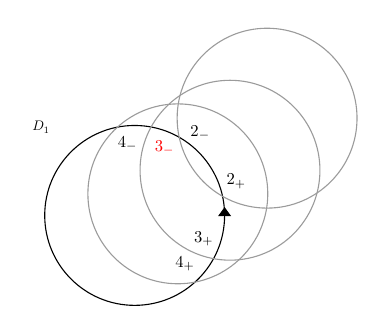
\begin{tikzpicture}[x=1pt,y=1pt,yscale=-1.3,xscale=1.3]
%uncomment if require: \path (0,95); %set diagram left start at 0, and has height of 95

%Shape: Circle [id:dp37777408295388804] 
\draw   (21,59.5) .. controls (21,45.69) and (32.19,34.5) .. (46,34.5) .. controls (59.81,34.5) and (71,45.69) .. (71,59.5) .. controls (71,73.31) and (59.81,84.5) .. (46,84.5) .. controls (32.19,84.5) and (21,73.31) .. (21,59.5) -- cycle ;
%Shape: Circle [id:dp4562198988843913] 
\draw  [color={rgb, 255:red, 155; green, 155; blue, 155 }  ,draw opacity=1 ] (47.5,46.94) .. controls (47.5,33.14) and (58.69,21.94) .. (72.5,21.94) .. controls (86.31,21.94) and (97.5,33.14) .. (97.5,46.94) .. controls (97.5,60.75) and (86.31,71.94) .. (72.5,71.94) .. controls (58.69,71.94) and (47.5,60.75) .. (47.5,46.94) -- cycle ;
%Shape: Circle [id:dp8913971633985722] 
\draw  [color={rgb, 255:red, 155; green, 155; blue, 155 }  ,draw opacity=1 ] (33,53.5) .. controls (33,39.69) and (44.19,28.5) .. (58,28.5) .. controls (71.81,28.5) and (83,39.69) .. (83,53.5) .. controls (83,67.31) and (71.81,78.5) .. (58,78.5) .. controls (44.19,78.5) and (33,67.31) .. (33,53.5) -- cycle ;
%Shape: Circle [id:dp05970043129919356] 
\draw  [color={rgb, 255:red, 155; green, 155; blue, 155 } ,draw opacity=1 ] (57.81,32.47) .. controls (57.81,18.66) and (69,7.47) .. (82.81,7.47) .. controls (96.62,7.47) and (107.81,18.66) .. (107.81,32.47) .. controls (107.81,46.27) and (96.62,57.47) .. (82.81,57.47) .. controls (69,57.47) and (57.81,46.27) .. (57.81,32.47) -- cycle ;
%Straight Lines [id:da04725899028195979] 
%\draw[densely dotted]  (21,59.5) -- (71,59.5) ;


%Flowchart: Extract [id:dp5267407418119328] 
\draw  [fill={rgb, 255:red, 0; green, 0; blue, 0 }  ,fill opacity=1 ] (71,57.45) -- (72.52,59.55) -- (69.48,59.55) -- cycle ;

\draw (60,73) node [scale=0.6]  {$4_+$};
% Text Node
\draw (65.22,66) node [scale=0.6]  {$3_+$};
% Text Node
\draw (74.22,50) node [scale=0.6]  {$2_+$};
% Text Node
\draw (64.22,36.56) node [scale=0.6]  {$2_-$};
% Text Node
\draw (54.32,40.66) node [scale=0.6,color=red]  {$3_-$};
% Text Node
\draw (44.02,39.56) node [scale=0.6]  {$4_-$};

% Text Node
\draw (20,35) node [scale=0.5]  {$D_{1}$};
\end{tikzpicture}

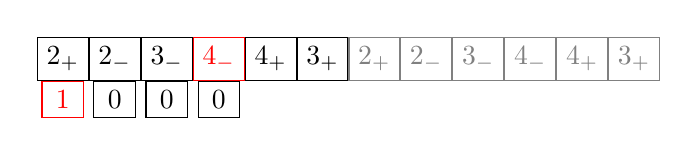
\begin{tikzpicture}

\matrix [matrix of nodes,row sep=,row sep=0mm,
column 1/.style={nodes={rectangle,draw,minimum width=1.5em, minimum height=0.5em}},
column 2/.style={nodes={rectangle,draw,minimum width=1.5em, minimum height=0.5em}},
column 3/.style={nodes={rectangle,draw,minimum width=1.5em, minimum height=0.5em}},
column 4/.style={nodes={rectangle,draw,minimum width=1.5em, color=red, minimum height=0.5em}},
column 5/.style={nodes={rectangle,draw,minimum width=1.5em, minimum height=0.5em}},
column 6/.style={nodes={rectangle,draw,minimum width=1.5em, minimum height=0.5em}},
column 7/.style={nodes={rectangle,draw,minimum width=1.5em, color=gray, minimum height=0.5em}},
column 8/.style={nodes={rectangle,draw,minimum width=1.5em, color=gray, minimum height=0.5em}},
column 9/.style={nodes={rectangle,draw,minimum width=1.5em, color=gray, minimum height=0.5em}},
column 10/.style={nodes={rectangle,draw,minimum width=1.5em, color=gray, minimum height=0.5em}},
column 11/.style={nodes={rectangle,draw,minimum width=1.5em, color=gray, minimum height=0.5em}},
column 12/.style={nodes={rectangle,draw,minimum width=1.5em, color=gray, minimum height=0.5em}}
] (O)
{
	$2_+$ & $2_-$ & $3_-$ & $4_-$ & $4_+$ & $3_+$ & $2_+$ & $2_-$ & $3_-$ & $4_-$ & $4_+$ & $3_+$\\
	|[color=red]|$1$ & |[color=black]|$0$ & |[color=black]|$0$ & |[color=black]|$0$\\
};

%\node at (-4,-0.5) {$0$};
%\node at (0,-0.5) {$2\pi$};
\end{tikzpicture}}
		
		\only<5>{\tikzset{every picture/.style={line width=0.75pt}} %set default line width to 0.75pt        

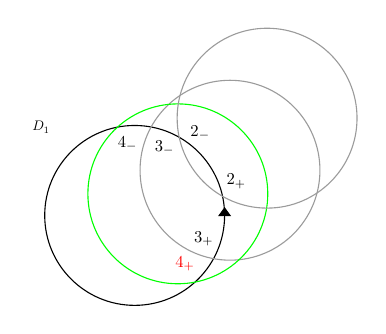
\begin{tikzpicture}[x=1pt,y=1pt,yscale=-1.3,xscale=1.3]
%uncomment if require: \path (0,95); %set diagram left start at 0, and has height of 95

%Shape: Circle [id:dp37777408295388804] 
\draw   (21,59.5) .. controls (21,45.69) and (32.19,34.5) .. (46,34.5) .. controls (59.81,34.5) and (71,45.69) .. (71,59.5) .. controls (71,73.31) and (59.81,84.5) .. (46,84.5) .. controls (32.19,84.5) and (21,73.31) .. (21,59.5) -- cycle ;
%Shape: Circle [id:dp4562198988843913] 
\draw  [color={rgb, 255:red, 155; green, 155; blue, 155 }  ,draw opacity=1 ] (47.5,46.94) .. controls (47.5,33.14) and (58.69,21.94) .. (72.5,21.94) .. controls (86.31,21.94) and (97.5,33.14) .. (97.5,46.94) .. controls (97.5,60.75) and (86.31,71.94) .. (72.5,71.94) .. controls (58.69,71.94) and (47.5,60.75) .. (47.5,46.94) -- cycle ;
%Shape: Circle [id:dp8913971633985722] 
\draw  [color=green  ,draw opacity=1 ] (33,53.5) .. controls (33,39.69) and (44.19,28.5) .. (58,28.5) .. controls (71.81,28.5) and (83,39.69) .. (83,53.5) .. controls (83,67.31) and (71.81,78.5) .. (58,78.5) .. controls (44.19,78.5) and (33,67.31) .. (33,53.5) -- cycle ;
%Shape: Circle [id:dp05970043129919356] 
\draw  [color={rgb, 255:red, 155; green, 155; blue, 155 } ,draw opacity=1 ] (57.81,32.47) .. controls (57.81,18.66) and (69,7.47) .. (82.81,7.47) .. controls (96.62,7.47) and (107.81,18.66) .. (107.81,32.47) .. controls (107.81,46.27) and (96.62,57.47) .. (82.81,57.47) .. controls (69,57.47) and (57.81,46.27) .. (57.81,32.47) -- cycle ;
%Straight Lines [id:da04725899028195979] 
%\draw[densely dotted]  (21,59.5) -- (71,59.5) ;


%Flowchart: Extract [id:dp5267407418119328] 
\draw  [fill={rgb, 255:red, 0; green, 0; blue, 0 }  ,fill opacity=1 ] (71,57.45) -- (72.52,59.55) -- (69.48,59.55) -- cycle ;


\draw (60,73) node [scale=0.6, color=red]  {$4_+$};
% Text Node
\draw (65.22,66) node [scale=0.6]  {$3_+$};
% Text Node
\draw (74.22,50) node [scale=0.6]  {$2_+$};
% Text Node
\draw (64.22,36.56) node [scale=0.6]  {$2_-$};
% Text Node
\draw (54.32,40.66) node [scale=0.6]  {$3_-$};
% Text Node
\draw (44.02,39.56) node [scale=0.6]  {$4_-$};

% Text Node
\draw (20,35) node [scale=0.5]  {$D_{1}$};
\end{tikzpicture}

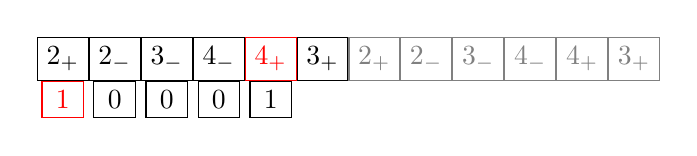
\begin{tikzpicture}

\matrix [matrix of nodes,row sep=,row sep=0mm,
column 1/.style={nodes={rectangle,draw,minimum width=1.5em, minimum height=0.5em}},
column 2/.style={nodes={rectangle,draw,minimum width=1.5em, minimum height=0.5em}},
column 3/.style={nodes={rectangle,draw,minimum width=1.5em, minimum height=0.5em}},
column 4/.style={nodes={rectangle,draw,minimum width=1.5em, minimum height=0.5em}},
column 5/.style={nodes={rectangle,draw,minimum width=1.5em, color=red, minimum height=0.5em}},
column 6/.style={nodes={rectangle,draw,minimum width=1.5em, minimum height=0.5em}},
column 7/.style={nodes={rectangle,draw,minimum width=1.5em, color=gray, minimum height=0.5em}},
column 8/.style={nodes={rectangle,draw,minimum width=1.5em, color=gray, minimum height=0.5em}},
column 9/.style={nodes={rectangle,draw,minimum width=1.5em, color=gray, minimum height=0.5em}},
column 10/.style={nodes={rectangle,draw,minimum width=1.5em, color=gray, minimum height=0.5em}},
column 11/.style={nodes={rectangle,draw,minimum width=1.5em, color=gray, minimum height=0.5em}},
column 12/.style={nodes={rectangle,draw,minimum width=1.5em, color=gray, minimum height=0.5em}}
] (O)
{
$2_+$ & $2_-$ & $3_-$ & $4_-$ & $4_+$ & $3_+$ & $2_+$ & $2_-$ & $3_-$ & $4_-$ & $4_+$ & $3_+$\\
|[color=red]|$1$ & |[color=black]|$0$ & |[color=black]|$0$ & |[color=black]|$0$ & |[color=black]|$1$\\
};

%\node at (-4,-0.5) {$0$};
%\node at (0,-0.5) {$2\pi$};
\end{tikzpicture}}
		\only<6>{\tikzset{every picture/.style={line width=0.75pt}} %set default line width to 0.75pt        

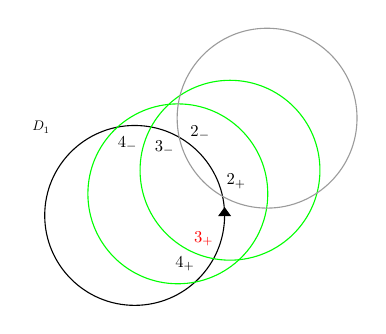
\begin{tikzpicture}[x=1pt,y=1pt,yscale=-1.3,xscale=1.3]
%uncomment if require: \path (0,95); %set diagram left start at 0, and has height of 95

%Shape: Circle [id:dp37777408295388804] 
\draw   (21,59.5) .. controls (21,45.69) and (32.19,34.5) .. (46,34.5) .. controls (59.81,34.5) and (71,45.69) .. (71,59.5) .. controls (71,73.31) and (59.81,84.5) .. (46,84.5) .. controls (32.19,84.5) and (21,73.31) .. (21,59.5) -- cycle ;


%Shape: Circle [id:dp4562198988843913] 
\draw  [color=green  ,draw opacity=1 ] (47.5,46.94) .. controls (47.5,33.14) and (58.69,21.94) .. (72.5,21.94) .. controls (86.31,21.94) and (97.5,33.14) .. (97.5,46.94) .. controls (97.5,60.75) and (86.31,71.94) .. (72.5,71.94) .. controls (58.69,71.94) and (47.5,60.75) .. (47.5,46.94) -- cycle ;


%Shape: Circle [id:dp8913971633985722] 
\draw  [color=green  ,draw opacity=1 ] (33,53.5) .. controls (33,39.69) and (44.19,28.5) .. (58,28.5) .. controls (71.81,28.5) and (83,39.69) .. (83,53.5) .. controls (83,67.31) and (71.81,78.5) .. (58,78.5) .. controls (44.19,78.5) and (33,67.31) .. (33,53.5) -- cycle ;


%Shape: Circle [id:dp05970043129919356] 
\draw  [color={rgb, 255:red, 155; green, 155; blue, 155 }  ,draw opacity=1 ] (57.81,32.47) .. controls (57.81,18.66) and (69,7.47) .. (82.81,7.47) .. controls (96.62,7.47) and (107.81,18.66) .. (107.81,32.47) .. controls (107.81,46.27) and (96.62,57.47) .. (82.81,57.47) .. controls (69,57.47) and (57.81,46.27) .. (57.81,32.47) -- cycle ;
%Straight Lines [id:da04725899028195979] 
%\draw[densely dotted]  (21,59.5) -- (71,59.5) ;


%Flowchart: Extract [id:dp5267407418119328] 
\draw  [fill={rgb, 255:red, 0; green, 0; blue, 0 }  ,fill opacity=1 ] (71,57.45) -- (72.52,59.55) -- (69.48,59.55) -- cycle ;


\draw (60,73) node [scale=0.6]  {$4_+$};
% Text Node
\draw (65.22,66) node [scale=0.6,color=red]  {$3_+$};
% Text Node
\draw (74.22,50) node [scale=0.6]  {$2_+$};
% Text Node
\draw (64.22,36.56) node [scale=0.6]  {$2_-$};
% Text Node
\draw (54.32,40.66) node [scale=0.6]  {$3_-$};
% Text Node
\draw (44.02,39.56) node [scale=0.6]  {$4_-$};

% Text Node
\draw (20,35) node [scale=0.5]  {$D_{1}$};
\end{tikzpicture}

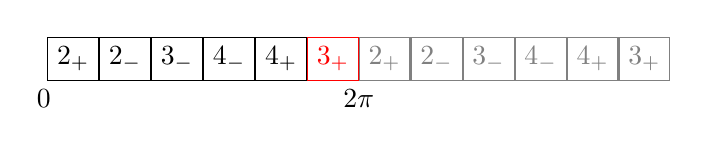
\begin{tikzpicture}

\matrix [matrix of nodes,row sep=,row sep=0mm,
column 1/.style={nodes={rectangle,draw,minimum width=1.5em, minimum height=0.5em}},
column 2/.style={nodes={rectangle,draw,minimum width=1.5em, minimum height=0.5em}},
column 3/.style={nodes={rectangle,draw,minimum width=1.5em, minimum height=0.5em}},
column 4/.style={nodes={rectangle,draw,minimum width=1.5em, minimum height=0.5em}},
column 5/.style={nodes={rectangle,draw,minimum width=1.5em, minimum height=0.5em}},
column 6/.style={nodes={rectangle,draw,minimum width=1.5em, color=red,minimum height=0.5em}},
column 7/.style={nodes={rectangle,draw,minimum width=1.5em, color=gray, minimum height=0.5em}},
column 8/.style={nodes={rectangle,draw,minimum width=1.5em, color=gray, minimum height=0.5em}},
column 9/.style={nodes={rectangle,draw,minimum width=1.5em, color=gray, minimum height=0.5em}},
column 10/.style={nodes={rectangle,draw,minimum width=1.5em, color=gray, minimum height=0.5em}},
column 11/.style={nodes={rectangle,draw,minimum width=1.5em, color=gray, minimum height=0.5em}},
column 12/.style={nodes={rectangle,draw,minimum width=1.5em, color=gray, minimum height=0.5em}}
] (O)
{
$2_+$ & $2_-$ & $3_-$ & $4_-$ & $4_+$ & $3_+$ & $2_+$ & $2_-$ & $3_-$ & $4_-$ & $4_+$ & $3_+$\\
	%$+$ & $-$ & $-$ & $-$ & $+$ & $+$\\
};

\node at (-4,-0.5) {$0$};
\node at (0,-0.5) {$2\pi$};
\end{tikzpicture}}
		\only<7>{\tikzset{every picture/.style={line width=0.75pt}} %set default line width to 0.75pt        

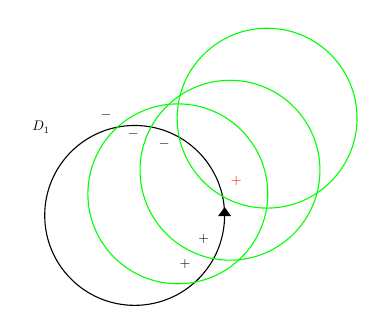
\begin{tikzpicture}[x=1pt,y=1pt,yscale=-1.3,xscale=1.3]
%uncomment if require: \path (0,95); %set diagram left start at 0, and has height of 95

%Shape: Circle [id:dp37777408295388804] 
\draw   (21,59.5) .. controls (21,45.69) and (32.19,34.5) .. (46,34.5) .. controls (59.81,34.5) and (71,45.69) .. (71,59.5) .. controls (71,73.31) and (59.81,84.5) .. (46,84.5) .. controls (32.19,84.5) and (21,73.31) .. (21,59.5) -- cycle ;


%Shape: Circle [id:dp4562198988843913] 
\draw  [color=green  ,draw opacity=1 ] (47.5,46.94) .. controls (47.5,33.14) and (58.69,21.94) .. (72.5,21.94) .. controls (86.31,21.94) and (97.5,33.14) .. (97.5,46.94) .. controls (97.5,60.75) and (86.31,71.94) .. (72.5,71.94) .. controls (58.69,71.94) and (47.5,60.75) .. (47.5,46.94) -- cycle ;


%Shape: Circle [id:dp8913971633985722] 
\draw  [color=green  ,draw opacity=1 ] (33,53.5) .. controls (33,39.69) and (44.19,28.5) .. (58,28.5) .. controls (71.81,28.5) and (83,39.69) .. (83,53.5) .. controls (83,67.31) and (71.81,78.5) .. (58,78.5) .. controls (44.19,78.5) and (33,67.31) .. (33,53.5) -- cycle ;


%Shape: Circle [id:dp05970043129919356] 
\draw  [color=green ,draw opacity=1 ] (57.81,32.47) .. controls (57.81,18.66) and (69,7.47) .. (82.81,7.47) .. controls (96.62,7.47) and (107.81,18.66) .. (107.81,32.47) .. controls (107.81,46.27) and (96.62,57.47) .. (82.81,57.47) .. controls (69,57.47) and (57.81,46.27) .. (57.81,32.47) -- cycle ;
%Straight Lines [id:da04725899028195979] 
%\draw[densely dotted]  (21,59.5) -- (71,59.5) ;


%Flowchart: Extract [id:dp5267407418119328] 
\draw  [fill={rgb, 255:red, 0; green, 0; blue, 0 }  ,fill opacity=1 ] (71,57.45) -- (72.52,59.55) -- (69.48,59.55) -- cycle ;

\draw (60,73) node [scale=0.5]  {$+$};
% Text Node
\draw (65.22,66) node [scale=0.5]  {$+$};
% Text Node
\draw (74.22,50) node [scale=0.5,color=red]  {$+$};
% Text Node
\draw (54.22,39.56) node [scale=0.5]  {$-$};
% Text Node
\draw (45.62,36.96) node [scale=0.5]  {$-$};
% Text Node
\draw (38.02,31.56) node [scale=0.5]  {$-$};


% Text Node
\draw (20,35) node [scale=0.5]  {$D_{1}$};
\end{tikzpicture}

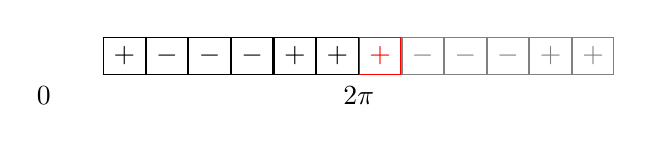
\begin{tikzpicture}

\matrix [matrix of nodes,row sep=,row sep=0mm,
column 1/.style={nodes={rectangle,draw,minimum width=1.5em, minimum height=0.5em}},
column 2/.style={nodes={rectangle,draw,minimum width=1.5em, minimum height=0.5em}},
column 3/.style={nodes={rectangle,draw,minimum width=1.5em, minimum height=0.5em}},
column 4/.style={nodes={rectangle,draw,minimum width=1.5em, minimum height=0.5em}},
column 5/.style={nodes={rectangle,draw,minimum width=1.5em, minimum height=0.5em}},
column 6/.style={nodes={rectangle,draw,minimum width=1.5em, minimum height=0.5em}},
column 7/.style={nodes={rectangle,draw,minimum width=1.5em, color=red, minimum height=0.5em}},
column 8/.style={nodes={rectangle,draw,minimum width=1.5em, color=gray, minimum height=0.5em}},
column 9/.style={nodes={rectangle,draw,minimum width=1.5em, color=gray, minimum height=0.5em}},
column 10/.style={nodes={rectangle,draw,minimum width=1.5em, color=gray, minimum height=0.5em}},
column 11/.style={nodes={rectangle,draw,minimum width=1.5em, color=gray, minimum height=0.5em}},
column 12/.style={nodes={rectangle,draw,minimum width=1.5em, color=gray, minimum height=0.5em}}
] (O)
{
	$+$ & $-$ & $-$ & $-$ & $+$ & $+$ & $+$ & $-$ & $-$ & $-$ & $+$ & $+$\\
	%$+$ & $-$ & $-$ & $-$ & $+$ & $+$\\
};

\node at (-4,-0.5) {$0$};
\node at (0,-0.5) {$2\pi$};
\end{tikzpicture}}
		\only<8>{\tikzset{every picture/.style={line width=0.75pt}} %set default line width to 0.75pt        

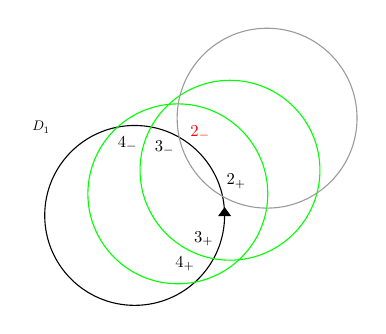
\begin{tikzpicture}[x=1pt,y=1pt,yscale=-1.3,xscale=1.3]
%uncomment if require: \path (0,95); %set diagram left start at 0, and has height of 95

%Shape: Circle [id:dp37777408295388804] 
\draw   (21,59.5) .. controls (21,45.69) and (32.19,34.5) .. (46,34.5) .. controls (59.81,34.5) and (71,45.69) .. (71,59.5) .. controls (71,73.31) and (59.81,84.5) .. (46,84.5) .. controls (32.19,84.5) and (21,73.31) .. (21,59.5) -- cycle ;


%Shape: Circle [id:dp4562198988843913] 
\draw  [color=green  ,draw opacity=1 ] (47.5,46.94) .. controls (47.5,33.14) and (58.69,21.94) .. (72.5,21.94) .. controls (86.31,21.94) and (97.5,33.14) .. (97.5,46.94) .. controls (97.5,60.75) and (86.31,71.94) .. (72.5,71.94) .. controls (58.69,71.94) and (47.5,60.75) .. (47.5,46.94) -- cycle ;


%Shape: Circle [id:dp8913971633985722] 
\draw  [color=green  ,draw opacity=1 ] (33,53.5) .. controls (33,39.69) and (44.19,28.5) .. (58,28.5) .. controls (71.81,28.5) and (83,39.69) .. (83,53.5) .. controls (83,67.31) and (71.81,78.5) .. (58,78.5) .. controls (44.19,78.5) and (33,67.31) .. (33,53.5) -- cycle ;


%Shape: Circle [id:dp05970043129919356] 
\draw  [color={rgb, 255:red, 155; green, 155; blue, 155 }  ,draw opacity=1 ] (57.81,32.47) .. controls (57.81,18.66) and (69,7.47) .. (82.81,7.47) .. controls (96.62,7.47) and (107.81,18.66) .. (107.81,32.47) .. controls (107.81,46.27) and (96.62,57.47) .. (82.81,57.47) .. controls (69,57.47) and (57.81,46.27) .. (57.81,32.47) -- cycle ;
%Straight Lines [id:da04725899028195979] 
%\draw[densely dotted]  (21,59.5) -- (71,59.5) ;


%Flowchart: Extract [id:dp5267407418119328] 
\draw  [fill={rgb, 255:red, 0; green, 0; blue, 0 }  ,fill opacity=1 ] (71,57.45) -- (72.52,59.55) -- (69.48,59.55) -- cycle ;

\draw (60,73) node [scale=0.6]  {$4_+$};
% Text Node
\draw (65.22,66) node [scale=0.6]  {$3_+$};
% Text Node
\draw (74.22,50) node [scale=0.6]  {$2_+$};
% Text Node
\draw (64.22,36.56) node [scale=0.6,color=red]  {$2_-$};
% Text Node
\draw (54.32,40.66) node [scale=0.6]  {$3_-$};
% Text Node
\draw (44.02,39.56) node [scale=0.6]  {$4_-$};


% Text Node
\draw (20,35) node [scale=0.5]  {$D_{1}$};
\end{tikzpicture}
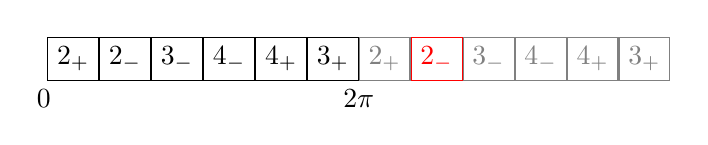
\begin{tikzpicture}

\matrix [matrix of nodes,row sep=,row sep=0mm,
column 1/.style={nodes={rectangle,draw,minimum width=1.5em, minimum height=0.5em}},
column 2/.style={nodes={rectangle,draw,minimum width=1.5em, minimum height=0.5em}},
column 3/.style={nodes={rectangle,draw,minimum width=1.5em, minimum height=0.5em}},
column 4/.style={nodes={rectangle,draw,minimum width=1.5em, minimum height=0.5em}},
column 5/.style={nodes={rectangle,draw,minimum width=1.5em, minimum height=0.5em}},
column 6/.style={nodes={rectangle,draw,minimum width=1.5em, minimum height=0.5em}},
column 7/.style={nodes={rectangle,draw,minimum width=1.5em, color=gray, minimum height=0.5em}},
column 8/.style={nodes={rectangle,draw,minimum width=1.5em, color=red, minimum height=0.5em}},
column 9/.style={nodes={rectangle,draw,minimum width=1.5em, color=gray, minimum height=0.5em}},
column 10/.style={nodes={rectangle,draw,minimum width=1.5em, color=gray, minimum height=0.5em}},
column 11/.style={nodes={rectangle,draw,minimum width=1.5em, color=gray, minimum height=0.5em}},
column 12/.style={nodes={rectangle,draw,minimum width=1.5em, color=gray, minimum height=0.5em}}
] (O)
{
$2_+$ & $2_-$ & $3_-$ & $4_-$ & $4_+$ & $3_+$ & $2_+$ & $2_-$ & $3_-$ & $4_-$ & $4_+$ & $3_+$\\
	%$+$ & $-$ & $-$ & $-$ & $+$ & $+$\\
};

\node at (-4,-0.5) {$0$};
\node at (0,-0.5) {$2\pi$};
\end{tikzpicture}}
		\only<9>{\tikzset{every picture/.style={line width=0.75pt}} %set default line width to 0.75pt        

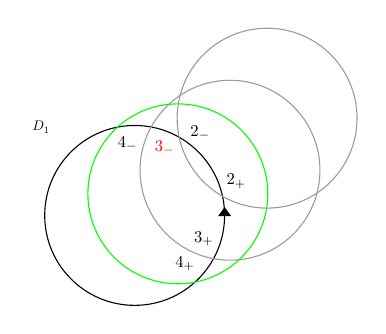
\begin{tikzpicture}[x=1pt,y=1pt,yscale=-1.3,xscale=1.3]
%uncomment if require: \path (0,95); %set diagram left start at 0, and has height of 95

%Shape: Circle [id:dp37777408295388804] 
\draw   (21,59.5) .. controls (21,45.69) and (32.19,34.5) .. (46,34.5) .. controls (59.81,34.5) and (71,45.69) .. (71,59.5) .. controls (71,73.31) and (59.81,84.5) .. (46,84.5) .. controls (32.19,84.5) and (21,73.31) .. (21,59.5) -- cycle ;


%Shape: Circle [id:dp4562198988843913] 
\draw  [color={rgb, 255:red, 155; green, 155; blue, 155 },draw opacity=1 ] (47.5,46.94) .. controls (47.5,33.14) and (58.69,21.94) .. (72.5,21.94) .. controls (86.31,21.94) and (97.5,33.14) .. (97.5,46.94) .. controls (97.5,60.75) and (86.31,71.94) .. (72.5,71.94) .. controls (58.69,71.94) and (47.5,60.75) .. (47.5,46.94) -- cycle ;


%Shape: Circle [id:dp8913971633985722] 
\draw  [color=green  ,draw opacity=1 ] (33,53.5) .. controls (33,39.69) and (44.19,28.5) .. (58,28.5) .. controls (71.81,28.5) and (83,39.69) .. (83,53.5) .. controls (83,67.31) and (71.81,78.5) .. (58,78.5) .. controls (44.19,78.5) and (33,67.31) .. (33,53.5) -- cycle ;


%Shape: Circle [id:dp05970043129919356] 
\draw  [color={rgb, 255:red, 155; green, 155; blue, 155 }  ,draw opacity=1 ] (57.81,32.47) .. controls (57.81,18.66) and (69,7.47) .. (82.81,7.47) .. controls (96.62,7.47) and (107.81,18.66) .. (107.81,32.47) .. controls (107.81,46.27) and (96.62,57.47) .. (82.81,57.47) .. controls (69,57.47) and (57.81,46.27) .. (57.81,32.47) -- cycle ;
%Straight Lines [id:da04725899028195979] 
%\draw[densely dotted]  (21,59.5) -- (71,59.5) ;


%Flowchart: Extract [id:dp5267407418119328] 
\draw  [fill={rgb, 255:red, 0; green, 0; blue, 0 }  ,fill opacity=1 ] (71,57.45) -- (72.52,59.55) -- (69.48,59.55) -- cycle ;

\draw (60,73) node [scale=0.6]  {$4_+$};
% Text Node
\draw (65.22,66) node [scale=0.6]  {$3_+$};
% Text Node
\draw (74.22,50) node [scale=0.6]  {$2_+$};
% Text Node
\draw (64.22,36.56) node [scale=0.6]  {$2_-$};
% Text Node
\draw (54.32,40.66) node [scale=0.6,color=red]  {$3_-$};
% Text Node
\draw (44.02,39.56) node [scale=0.6]  {$4_-$};

% Text Node
\draw (20,35) node [scale=0.5]  {$D_{1}$};
\end{tikzpicture}

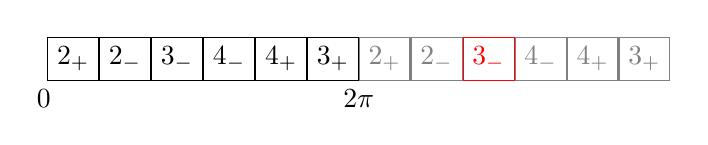
\begin{tikzpicture}

\matrix [matrix of nodes,row sep=,row sep=0mm,
column 1/.style={nodes={rectangle,draw,minimum width=1.5em, minimum height=0.5em}},
column 2/.style={nodes={rectangle,draw,minimum width=1.5em, minimum height=0.5em}},
column 3/.style={nodes={rectangle,draw,minimum width=1.5em, minimum height=0.5em}},
column 4/.style={nodes={rectangle,draw,minimum width=1.5em, minimum height=0.5em}},
column 5/.style={nodes={rectangle,draw,minimum width=1.5em, minimum height=0.5em}},
column 6/.style={nodes={rectangle,draw,minimum width=1.5em, minimum height=0.5em}},
column 7/.style={nodes={rectangle,draw,minimum width=1.5em, color=gray, minimum height=0.5em}},
column 8/.style={nodes={rectangle,draw,minimum width=1.5em, color=gray, minimum height=0.5em}},
column 9/.style={nodes={rectangle,draw,minimum width=1.5em, color=red, minimum height=0.5em}},
column 10/.style={nodes={rectangle,draw,minimum width=1.5em, color=gray, minimum height=0.5em}},
column 11/.style={nodes={rectangle,draw,minimum width=1.5em, color=gray, minimum height=0.5em}},
column 12/.style={nodes={rectangle,draw,minimum width=1.5em, color=gray, minimum height=0.5em}}
] (O)
{
$2_+$ & $2_-$ & $3_-$ & $4_-$ & $4_+$ & $3_+$ & $2_+$ & $2_-$ & $3_-$ & $4_-$ & $4_+$ & $3_+$\\
	%$+$ & $-$ & $-$ & $-$ & $+$ & $+$\\
};

\node at (-4,-0.5) {$0$};
\node at (0,-0.5) {$2\pi$};
\end{tikzpicture}}
		\only<10>{\tikzset{every picture/.style={line width=0.75pt}} %set default line width to 0.75pt        

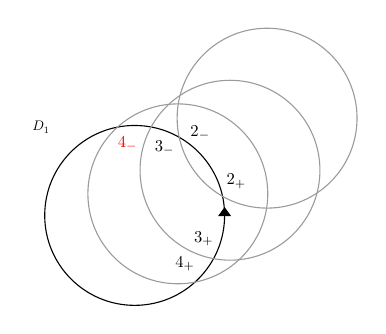
\begin{tikzpicture}[x=1pt,y=1pt,yscale=-1.3,xscale=1.3]
%uncomment if require: \path (0,95); %set diagram left start at 0, and has height of 95

%Shape: Circle [id:dp37777408295388804] 
\draw   (21,59.5) .. controls (21,45.69) and (32.19,34.5) .. (46,34.5) .. controls (59.81,34.5) and (71,45.69) .. (71,59.5) .. controls (71,73.31) and (59.81,84.5) .. (46,84.5) .. controls (32.19,84.5) and (21,73.31) .. (21,59.5) -- cycle ;


%Shape: Circle [id:dp4562198988843913] 
\draw  [color={rgb, 255:red, 155; green, 155; blue, 155 },draw opacity=1 ] (47.5,46.94) .. controls (47.5,33.14) and (58.69,21.94) .. (72.5,21.94) .. controls (86.31,21.94) and (97.5,33.14) .. (97.5,46.94) .. controls (97.5,60.75) and (86.31,71.94) .. (72.5,71.94) .. controls (58.69,71.94) and (47.5,60.75) .. (47.5,46.94) -- cycle ;


%Shape: Circle [id:dp8913971633985722] 
\draw  [color={rgb, 255:red, 155; green, 155; blue, 155 } ,draw opacity=1 ] (33,53.5) .. controls (33,39.69) and (44.19,28.5) .. (58,28.5) .. controls (71.81,28.5) and (83,39.69) .. (83,53.5) .. controls (83,67.31) and (71.81,78.5) .. (58,78.5) .. controls (44.19,78.5) and (33,67.31) .. (33,53.5) -- cycle ;


%Shape: Circle [id:dp05970043129919356] 
\draw  [color={rgb, 255:red, 155; green, 155; blue, 155 }  ,draw opacity=1 ] (57.81,32.47) .. controls (57.81,18.66) and (69,7.47) .. (82.81,7.47) .. controls (96.62,7.47) and (107.81,18.66) .. (107.81,32.47) .. controls (107.81,46.27) and (96.62,57.47) .. (82.81,57.47) .. controls (69,57.47) and (57.81,46.27) .. (57.81,32.47) -- cycle ;
%Straight Lines [id:da04725899028195979] 
%\draw[densely dotted]  (21,59.5) -- (71,59.5) ;


%Flowchart: Extract [id:dp5267407418119328] 
\draw  [fill={rgb, 255:red, 0; green, 0; blue, 0 }  ,fill opacity=1 ] (71,57.45) -- (72.52,59.55) -- (69.48,59.55) -- cycle ;

\draw (60,73) node [scale=0.6]  {$4_+$};
% Text Node
\draw (65.22,66) node [scale=0.6]  {$3_+$};
% Text Node
\draw (74.22,50) node [scale=0.6]  {$2_+$};
% Text Node
\draw (64.22,36.56) node [scale=0.6]  {$2_-$};
% Text Node
\draw (54.32,40.66) node [scale=0.6]  {$3_-$};
% Text Node
\draw (44.02,39.56) node [scale=0.6,color=red]  {$4_-$};


% Text Node
\draw (20,35) node [scale=0.5]  {$D_{1}$};
\end{tikzpicture}

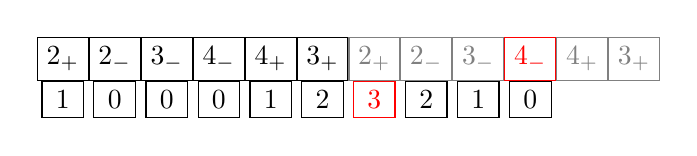
\begin{tikzpicture}

\matrix [matrix of nodes,row sep=,row sep=0mm,
column 1/.style={nodes={rectangle,draw,minimum width=1.5em, minimum height=0.5em}},
column 2/.style={nodes={rectangle,draw,minimum width=1.5em, minimum height=0.5em}},
column 3/.style={nodes={rectangle,draw,minimum width=1.5em, minimum height=0.5em}},
column 4/.style={nodes={rectangle,draw,minimum width=1.5em, minimum height=0.5em}},
column 5/.style={nodes={rectangle,draw,minimum width=1.5em, minimum height=0.5em}},
column 6/.style={nodes={rectangle,draw,minimum width=1.5em, minimum height=0.5em}},
column 7/.style={nodes={rectangle,draw,minimum width=1.5em, color=gray, minimum height=0.5em}},
column 8/.style={nodes={rectangle,draw,minimum width=1.5em, color=gray, minimum height=0.5em}},
column 9/.style={nodes={rectangle,draw,minimum width=1.5em, color=gray, minimum height=0.5em}},
column 10/.style={nodes={rectangle,draw,minimum width=1.5em, color=red, minimum height=0.5em}},
column 11/.style={nodes={rectangle,draw,minimum width=1.5em, color=gray, minimum height=0.5em}},
column 12/.style={nodes={rectangle,draw,minimum width=1.5em, color=gray, minimum height=0.5em}}
] (O)
{
$2_+$ & $2_-$ & $3_-$ & $4_-$ & $4_+$ & $3_+$ & $2_+$ & $2_-$ & $3_-$ & $4_-$ & $4_+$ & $3_+$\\
|[color=black]|$1$ & |[color=black]|$0$ & |[color=black]|$0$ & |[color=black]|$0$ & |[color=black]|$1$ & |[color=black]|$2$ & |[color=red]|$3$ & |[color=black]|$2$ & |[color=black]|$1$ &|[color=black]|$0$\\
};

%\node at (-4,-0.5) {$0$};
%\node at (0,-0.5) {$2\pi$};
\end{tikzpicture}}
			\source{Elaborated by the author.}
	\end{figure}
\end{frame}


\begin{frame}{Maximum Weight Clique Problem}{Algorithm}
	
	The run-time complexity of the algorithm is $\bigO(n^2\log{n})$.
	
	\begin{itemize}
		\item There are $\bigO(n^2)$ intersections among $n$ disks.
		
		\item Sorting takes $\bigO(n^2\log{n})$.
		
		\item The traversal takes $\bigO(n)$ for every disk.
		
		\item It can be implemented in $\bigO(K\log{n})$ where $K$ is the number of intersections \autocite{bentley:1979}.
		
		\item The algorithm is basically finding the most number of overlapping intervals $n$ times.

	\end{itemize}
	As it was mentioned, the solution found by this algorithm is a solution for the Maximal Covering by One Disk.

\end{frame}

\begin{frame}{Maximum Covering by Disks}{Multiple disks}
	
	Works found in the literature:
	
	\begin{itemize}
		\item In \autocite{cabello:2006} a $\bigO(n^{2m-1})$ algorithm was proposed. Also a $(1-\epsilon)-$approximation that runs in $\bigO(n\log{n})$ was introduced.
		
		\item In \autocite{zhou} a heuristic method using an algorithm called mean-shift was developed. The mean-shift algorithm converges to a local density maxima of any probability distribution and it is used to find a smaller candidate list of centers for the disks.
	\end{itemize}
	
	Because of the similarities, we will discuss only the multiple ellipses algorithm later.
	
\end{frame}
\section{Maximal Covering by Ellipses}

\begin{frame}{Ellipses}
	
	\begin{block}{Ellipse}
		Given a center $c \in \R^2$ and $Q \in \R^ {2x2}$ a positive definite matrix, an ellipse is the set of points that satisfy
		
		\begin{equation*}
		||u-c||_Q^2 = (u-c)^TQ(u-c) = 1,
		\end{equation*}
		
		with $\le$ representing the set of covered points.
	\end{block}
	
	\begin{block}{Axis-parallel ellipse}
		Any $2$ by $2$ diagonal p.d. matrix determines an axis-parallel ellipse, which can also be described by
		
		\begin{equation*}
		\frac{(x-c_x)^2}{a^2} + \frac{(y-c_y)^2}{b^2} = 1,
		\end{equation*}
		
		where $(a,b)$ are the shape parameters and $c=(c_x,c_y)$ is the center.
	\end{block}
	
\end{frame}

\begin{frame}{Ellipses}
	\begin{figure}[H]
		\centering
		
		\caption{The ellipse seen as just a linear transformation of a circle.}
		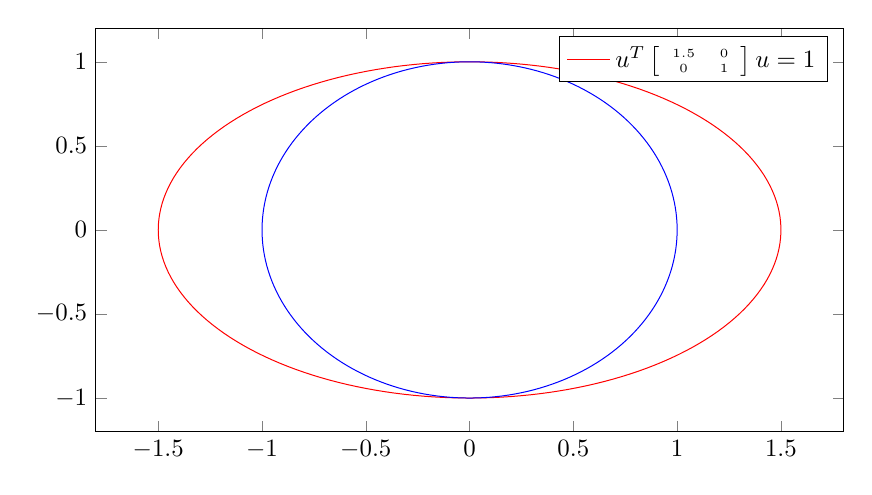
\begin{tikzpicture}[scale=0.9]
\begin{axis}[
    %axis lines = left,
    xlabel = ,
    ylabel = ,
    width=\textwidth,
    height=\axisdefaultheight
]

%Below the red parabola is defined
\addplot [domain=-pi:pi,samples=200,red]({1.5*cos(deg(x))}, {1*sin(deg(x))});

\addlegendentry{$\tiny u^T\left[\begin{array}{cc}
		1.5 & 0\\
		0 & 1
	\end{array}\right]u = 1$}
\addplot [domain=-pi:pi,samples=200,blue]({sin(deg(x))}, {cos(deg(x))});
\end{axis}
\end{tikzpicture}
		\source{Elaborated by the author.}
		\label{fig:3ellipses_intersect}
		
	\end{figure}
\end{frame}



\begin{frame}{Maximal Covering by Ellipses}{One ellipse}
	Let $MCE(\Pp, a, b)$ be an instance of the maximal covering by one ellipse, with $E$ being an ellipse with shape parameters $(a,b) \in \R_{>0}^2$, and $\Pp=\{p_1,\dots,p_n\}$ is a set of $n$ points with each point having a positive weight $w_i$, an optimal solution of $MCE(\Pp, a, b)$ is given by
	
	\begin{equation*}
	\max_q w(\Pp \cap E(q)),
	\end{equation*}

	\begin{itemize}
		\item $E(q)$ is an axis-parallel ellipse with center point $q$.
		\item $w(A)$, $A \subset \Pp$, is the sum of the weights of every point in $\Pp$.
		\item Same algorithm for one disk.
	\end{itemize}

\end{frame}

\begin{frame}{Maximal Covering by Ellipses}{One ellipse}
\begin{figure}[H]
	\centering
	
	\caption{Intersection points of $E_1$ with $E_2$ and $E_3$ along with opening and closing angles indicators.}
	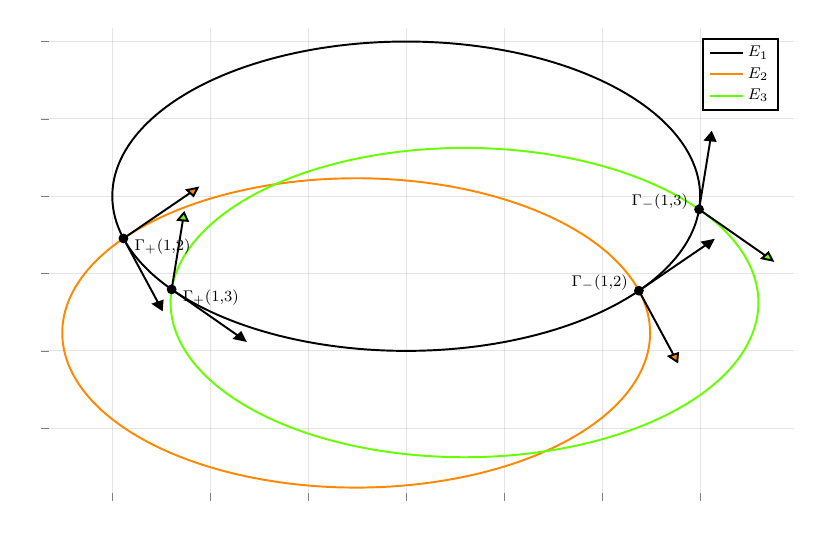
\begin{tikzpicture}[scale=0.7]
\begin{axis}[height = {101.6mm}, ylabel = {}, xmin = {-3.7279015473763786}, xmax = {3.956162987575968}, ymax = {2.172965670438345}, xlabel = {}, unbounded coords=jump,scaled x ticks = false,xlabel style = {font = {\fontsize{11 pt}{14.3 pt}\selectfont}, color = {rgb,1:red,0.00000000;green,0.00000000;blue,0.00000000}, draw opacity = 1.0, rotate = 0.0},xmajorgrids = true,xtick = {-3.0,-2.0,-1.0,0.0,1.0,2.0,3.0},xticklabels = {},xtick align = inside,xticklabel style = {font = {\fontsize{8 pt}{10.4 pt}\selectfont}, color = {rgb,1:red,0.00000000;green,0.00000000;blue,0.00000000}, draw opacity = 1.0, rotate = 0.0},x grid style = {color = {rgb,1:red,0.00000000;green,0.00000000;blue,0.00000000},
draw opacity = 0.1,
line width = 0.5,
solid},axis lines* = left,separate axis lines,x axis line style = {draw opacity = 0},scaled y ticks = false,ylabel style = {font = {\fontsize{11 pt}{14.3 pt}\selectfont}, color = {rgb,1:red,0.00000000;green,0.00000000;blue,0.00000000}, draw opacity = 1.0, rotate = 0.0},ymajorgrids = true,ytick = {-3.0,-2.0,-1.0,0.0,1.0,2.0},yticklabels = {},ytick align = inside,yticklabel style = {font = {\fontsize{8 pt}{10.4 pt}\selectfont}, color = {rgb,1:red,0.00000000;green,0.00000000;blue,0.00000000}, draw opacity = 1.0, rotate = 0.0},y grid style = {color = {rgb,1:red,0.00000000;green,0.00000000;blue,0.00000000},
draw opacity = 0.1,
line width = 0.5,
solid},axis lines* = left,separate axis lines,y axis line style = {draw opacity = 0},    xshift = 0.0mm,
    yshift = 0.0mm,
    axis background/.style={fill={rgb,1:red,1.00000000;green,1.00000000;blue,1.00000000}}
,legend style = {color = {rgb,1:red,0.00000000;green,0.00000000;blue,0.00000000},
draw opacity = 1.0,
line width = 1,
solid,fill = {rgb,1:red,1.00000000;green,1.00000000;blue,1.00000000},font = {\fontsize{8 pt}{10.4 pt}\selectfont}},colorbar style={title=}, ymin = {-3.9406895045294608}, width = {152.4mm}]\addplot+ [color = {rgb,1:red,0.00000000;green,0.00000000;blue,0.00000000},
draw opacity = 1.0,
line width = 1,
solid,mark = none,
mark size = 2.0,
mark options = {
    color = {rgb,1:red,0.00000000;green,0.00000000;blue,0.00000000}, draw opacity = 1.0,
    fill = {rgb,1:red,0.00000000;green,0.00000000;blue,0.00000000}, fill opacity = 1.0,
    line width = 1,
    rotate = 0,
    solid
}]coordinates {
(3.0, 0.0)
(2.9985047673785212, 0.06313709952962106)
(2.99402055999448, 0.1262112626253473)
(2.9865518478033177, 0.18915961558968988)
(2.9761060757797733, 0.2519194101354351)
(2.962693656496571, 0.31442808593450156)
(2.9463279597449414, 0.37662333297943573)
(2.9270252992073207, 0.43844315369538267)
(2.9048049161955216, 0.4998259247406167)
(2.879688960470571, 0.5607104584340288)
(2.8517024681633485, 0.6210360637483376)
(2.8208733368180265, 0.6807426068082256)
(2.787232297583192, 0.7397705708330936)
(2.7508128845783664, 0.7980611154646818)
(2.7116514014664705, 0.8555561354204192)
(2.669786885265541, 0.9121983184140319)
(2.625261067435781, 0.9679312022856775)
(2.578118332280736, 1.0226992312846535)
(2.528405672704052, 1.076447811448577)
(2.4761726433659286, 1.1291233650238361)
(2.421471311285956, 1.1806733838730568)
(2.3643562039415773, 1.2310464818163585)
(2.3048842549139126, 1.2801924458542142)
(2.2431147471351274, 1.3280622862208624)
(2.1791092537939183, 1.3746082852183685)
(2.1129315769580166, 1.4197840447826657)
(2.0446476839749015, 1.4635445327341534)
(1.974325641714113, 1.505846127666754)
(1.902035548716716, 1.546646662430678)
(1.82784946531955, 1.5859054661655572)
(1.7518413418239187, 1.6235834048420414)
(1.6740869447803206, 1.6596429202714515)
(1.5946637814627043, 1.6940480675445977)
(1.5136510226075326, 1.7267645508624465)
(1.4311294234946685, 1.7577597577229207)
(1.3471812434487604, 1.7870027914297482)
(1.261890163841353, 1.8144645018909626)
(1.1753412046754794, 1.840117514676349)
(1.0876206398358734, 1.8639362583048695)
(0.9988159110892831, 1.885896989734874)
(0.9090155409206182, 1.9059778180316784)
(0.8183090442918096, 1.9241587261889257)
(0.7267868394113495, 1.9404215910819727)
(0.6345401576034572, 1.9547502015334144)
(0.541660952366707, 1.9671302744727397)
(0.4482418077127828, 1.9775494691740052)
(0.35437584587672416, 1.9859973995573392)
(0.26015663449065285, 1.9924656445420135)
(0.1656780933135245, 1.9969477564407576)
(0.0710344006098723, 1.9994392673869559)
(-0.02368010072913993, 1.9999376937883127)
(-0.1183709972287581, 1.9984425388025513)
(-0.21294389894404733, 1.9949552928326777)
(-0.3073045335498399, 1.9894794320413138)
(-0.40135884031343716, 1.9820204148855842)
(-0.49501306385639726, 1.9725856766760055)
(-0.588173847611934, 1.9611846221648082)
(-0.68074832688477, 1.9478286161710756)
(-0.7726442214206901, 1.9325309722520436)
(-0.8637699273934991, 1.9153069394318591)
(-0.9540346087177143, 1.896173687001019)
(-1.043348287595947, 1.8751502874016501)
(-1.1316219342107279, 1.8522576972156826)
(-1.2187675554713666, 1.8275187362748735)
(-1.304698282727379, 1.8009580649135033)
(-1.389328458361043, 1.7726021593864174)
(-1.4725737211727805, 1.7424792854769193)
(-1.5543510904742317, 1.710619470320824)
(-1.6345790488052114, 1.6770544724747547)
(-1.713177623192084, 1.6418177502585252)
(-1.7900684648665677, 1.604944428403156)
(-1.8651749273654852, 1.566471263037781)
(-1.9384221429336286, 1.5264366050503373)
(-2.009737097153566, 1.484880361858566)
(-2.079048701727995, 1.4418439576294326)
(-2.1462878653421136, 1.3973702919866131)
(-2.2113875625353363, 1.3515036972472176)
(-2.274282900513736, 1.3042898942303736)
(-2.3349111838365904, 1.2557759466817167)
(-2.393211976912558, 1.206010214359229)
(-2.449127164243197, 1.1550423048271772)
(-2.502601008353752, 1.1029230240062151)
(-2.5535802053534837, 1.0497043255289369)
(-2.6020139380701437, 0.9954392589513668)
(-2.6478539267056407, 0.9401819168720059)
(-2.6910544769623908, 0.8839873810111583)
(-2.7315725255923864, 0.8269116673042683)
(-2.7693676833235816, 0.769011670064022)
(-2.8044022751207947, 0.7103451052668572)
(-2.8366413777410013, 0.6509704530204232)
(-2.8660528545455843, 0.5909468992693401)
(-2.8926073875348353, 0.5303342767973575)
(-2.916278506572771, 0.46919300558473775)
(-2.9370426157731435, 0.4075840325803047)
(-2.954879017020331, 0.3455687709481997)
(-2.9697699306016716, 0.28320903884990317)
(-2.9817005129306633, 0.22056699782255015)
(-2.9906588713433795, 0.1577050908149532)
(-2.996636075953331, 0.09468597994311641)
(-2.9996261685529717, 0.03157248402727453)
(-2.9996261685529717, -0.031572484027274035)
(-2.996636075953331, -0.09468597994311592)
(-2.9906588713433795, -0.1577050908149527)
(-2.9817005129306637, -0.22056699782254965)
(-2.9697699306016716, -0.2832090388499027)
(-2.9548790170203314, -0.34556877094819927)
(-2.9370426157731435, -0.40758403258030423)
(-2.916278506572771, -0.46919300558473725)
(-2.8926073875348353, -0.530334276797357)
(-2.866052854545585, -0.5909468992693396)
(-2.8366413777410013, -0.6509704530204228)
(-2.804402275120795, -0.7103451052668568)
(-2.769367683323582, -0.7690116700640215)
(-2.7315725255923864, -0.8269116673042679)
(-2.6910544769623908, -0.8839873810111578)
(-2.647853926705641, -0.9401819168720055)
(-2.6020139380701437, -0.9954392589513663)
(-2.5535802053534837, -1.0497043255289367)
(-2.5026010083537527, -1.1029230240062147)
(-2.4491271642431975, -1.155042304827177)
(-2.393211976912559, -1.2060102143592286)
(-2.3349111838365904, -1.2557759466817162)
(-2.274282900513737, -1.3042898942303731)
(-2.211387562535337, -1.3515036972472174)
(-2.1462878653421145, -1.3973702919866127)
(-2.079048701727996, -1.4418439576294324)
(-2.0097370971535664, -1.4848803618585658)
(-1.9384221429336304, -1.5264366050503364)
(-1.8651749273654858, -1.5664712630377808)
(-1.7900684648665695, -1.604944428403155)
(-1.713177623192085, -1.641817750258525)
(-1.634579048805211, -1.677054472474755)
(-1.5543510904742333, -1.7106194703208233)
(-1.4725737211727812, -1.742479285476919)
(-1.389328458361045, -1.7726021593864167)
(-1.3046982827273796, -1.800958064913503)
(-1.2187675554713666, -1.8275187362748735)
(-1.131621934210729, -1.8522576972156821)
(-1.0433482875959472, -1.8751502874016501)
(-0.9540346087177163, -1.8961736870010186)
(-0.8637699273935, -1.915306939431859)
(-0.7726442214206894, -1.9325309722520438)
(-0.6807483268847714, -1.9478286161710754)
(-0.5881738476119341, -1.9611846221648082)
(-0.4950130638563993, -1.9725856766760053)
(-0.4013588403134378, -1.9820204148855842)
(-0.3073045335498393, -1.989479432041314)
(-0.2129438989440487, -1.9949552928326775)
(-0.11837099722875816, -1.9984425388025513)
(-0.023680100729141333, -1.9999376937883127)
(0.07103440060987157, -1.9994392673869559)
(0.1656780933135251, -1.9969477564407576)
(0.2601566344906514, -1.9924656445420135)
(0.3543758458767241, -1.9859973995573392)
(0.44824180771278144, -1.9775494691740052)
(0.5416609523667063, -1.96713027447274)
(0.6345401576034577, -1.9547502015334144)
(0.7267868394113488, -1.9404215910819727)
(0.8183090442918095, -1.9241587261889257)
(0.9090155409206169, -1.9059778180316789)
(0.998815911089283, -1.885896989734874)
(1.0876206398358716, -1.8639362583048702)
(1.1753412046754788, -1.840117514676349)
(1.261890163841353, -1.8144645018909626)
(1.3471812434487593, -1.7870027914297486)
(1.4311294234946685, -1.7577597577229207)
(1.5136510226075308, -1.7267645508624474)
(1.5946637814627036, -1.694048067544598)
(1.6740869447803208, -1.6596429202714515)
(1.7518413418239178, -1.6235834048420419)
(1.82784946531955, -1.5859054661655572)
(1.9020355487167147, -1.546646662430679)
(1.9743256417141124, -1.5058461276667543)
(2.044647683974902, -1.4635445327341534)
(2.1129315769580157, -1.4197840447826664)
(2.179109253793918, -1.3746082852183685)
(2.243114747135126, -1.3280622862208633)
(2.3048842549139117, -1.2801924458542147)
(2.3643562039415773, -1.231046481816358)
(2.4214713112859556, -1.1806733838730574)
(2.4761726433659286, -1.1291233650238361)
(2.528405672704051, -1.076447811448578)
(2.5781183322807357, -1.0226992312846537)
(2.6252610674357815, -0.9679312022856771)
(2.66978688526554, -0.9121983184140325)
(2.7116514014664705, -0.8555561354204191)
(2.750812884578366, -0.7980611154646828)
(2.7872322975831914, -0.7397705708330939)
(2.820873336818026, -0.680742606808227)
(2.8517024681633485, -0.6210360637483382)
(2.879688960470571, -0.5607104584340287)
(2.904804916195521, -0.4998259247406176)
(2.9270252992073207, -0.4384431536953829)
(2.946327959744941, -0.37662333297943695)
(2.9626936564965707, -0.3144280859345021)
(2.9761060757797737, -0.25191941013543495)
(2.9865518478033177, -0.18915961558969077)
(2.99402055999448, -0.12621126262534743)
(2.9985047673785212, -0.06313709952962226)
(3.0, -4.898587196589413e-16)
};
\addlegendentry{$E_1$}
\addplot+ [color = {rgb,1:red,1.00000000;green,0.53160000;blue,0.00000000},
draw opacity = 1.0,
line width = 1,
solid,mark = none,
mark size = 2.0,
mark options = {
    color = {rgb,1:red,0.00000000;green,0.00000000;blue,0.00000000}, draw opacity = 1.0,
    fill = {rgb,1:red,1.00000000;green,0.53160000;blue,0.00000000}, fill opacity = 1.0,
    line width = 1,
    rotate = 0,
    solid
}]coordinates {
(2.489198145750716, -1.7677238340911159)
(2.487702913129237, -1.704586734561495)
(2.483218705745196, -1.6415125714657686)
(2.4757499935540337, -1.578564218501426)
(2.4653042215304892, -1.5158044239556807)
(2.451891802247287, -1.4532957481566142)
(2.4355261054956574, -1.3911005011116802)
(2.4162234449580366, -1.3292806803957333)
(2.3940030619462376, -1.2678979093504992)
(2.368887106221287, -1.207013375657087)
(2.3409006139140645, -1.1466877703427782)
(2.3100714825687425, -1.0869812272828903)
(2.2764304433339078, -1.0279532632580222)
(2.2400110303290823, -0.969662718626434)
(2.2008495472171865, -0.9121676986706967)
(2.158985031016257, -0.855525515677084)
(2.114459213186497, -0.7997926318054384)
(2.067316478031452, -0.7450246028064624)
(2.0176038184547678, -0.691276022642539)
(1.9653707891166445, -0.6386004690672797)
(1.910669457036672, -0.5870504502180591)
(1.8535543496922933, -0.5366773522747574)
(1.7940824006646285, -0.4875313882369017)
(1.7323128928858433, -0.43966154787025347)
(1.6683073995446343, -0.39311554887274736)
(1.6021297227087326, -0.34793978930845015)
(1.5338458297256174, -0.3041793013569625)
(1.4635237874648293, -0.2618777064243618)
(1.3912336944674322, -0.22107717166043783)
(1.317047611070266, -0.18181836792555872)
(1.2410394875746347, -0.14414042924907444)
(1.1632850905310366, -0.10808091381966434)
(1.0838619272134205, -0.0736757665465182)
(1.0028491683582486, -0.040959283228669374)
(0.9203275692453846, -0.009964076368195185)
(0.8363793891994765, 0.019278957338632274)
(0.7510883095920692, 0.04674066779984676)
(0.6645393504261955, 0.07239368058523321)
(0.5768187855865895, 0.09621242421375364)
(0.4880140568399992, 0.11817315564375819)
(0.3982136866713343, 0.13825398394056254)
(0.3075071900425257, 0.1564348920978098)
(0.21598498516206555, 0.17269775699085677)
(0.12373830335417324, 0.1870263674422985)
(0.030859098117423045, 0.1994064403816238)
(-0.0625600465365011, 0.20982563508288932)
(-0.15642600837255977, 0.21827356546622334)
(-0.2506452197586311, 0.22474181045089758)
(-0.3451237609357594, 0.22922392234964173)
(-0.4397674536394116, 0.23171543329584)
(-0.5344819549784239, 0.23221385969719677)
(-0.629172851478042, 0.2307187047114354)
(-0.7237457531933312, 0.2272314587415618)
(-0.8181063877991238, 0.22175559795019795)
(-0.9121606945627211, 0.21429658079446834)
(-1.0058149181056812, 0.2048618425848896)
(-1.0989757018612178, 0.19346078807369227)
(-1.1915501811340539, 0.18010478207995972)
(-1.283446075669974, 0.16480713816092774)
(-1.374571781642783, 0.14758310534074326)
(-1.464836462966998, 0.12844985290990318)
(-1.554150141845231, 0.10742645331053424)
(-1.642423788460012, 0.08453386312456668)
(-1.7295694097206504, 0.0597949021837576)
(-1.815500136976663, 0.03323423082238741)
(-1.9001303126103268, 0.004878325295301522)
(-1.9833755754220643, -0.02524454861419656)
(-2.0651529447235157, -0.05710436377029193)
(-2.1453809030544955, -0.09066936161636119)
(-2.223979477441368, -0.12590608383259072)
(-2.3008703191158517, -0.1627794056879599)
(-2.375976781614769, -0.20125257105333483)
(-2.4492239971829126, -0.2412872290407786)
(-2.52053895140285, -0.2828434722325499)
(-2.589850555977279, -0.32587987646168326)
(-2.6570897195913976, -0.3703535421045028)
(-2.7221894167846203, -0.41622013684389825)
(-2.78508475476302, -0.4634339398607423)
(-2.8457130380858744, -0.5119478874093992)
(-2.904013831161842, -0.5617136197318868)
(-2.959929018492481, -0.6126815292639387)
(-3.0134028626030362, -0.6648008100849008)
(-3.0643820596027678, -0.718019508562179)
(-3.1128157923194277, -0.7722845751397491)
(-3.1586557809549247, -0.82754191721911)
(-3.201856331211675, -0.8837364530799576)
(-3.2423743798416704, -0.9408121667868475)
(-3.2801695375728657, -0.9987121640270938)
(-3.3152041293700787, -1.0573787288242587)
(-3.3474432319902854, -1.1167533810706927)
(-3.3768547087948684, -1.1767769348217758)
(-3.4034092417841193, -1.2373895572937585)
(-3.427080360822055, -1.2985308285063781)
(-3.4478444700224276, -1.3601398015108113)
(-3.465680871269615, -1.4221550631429163)
(-3.4805717848509556, -1.4845147952412128)
(-3.4925023671799473, -1.5471568362685657)
(-3.5014607255926635, -1.6100187432761626)
(-3.507437930202615, -1.6730378541479995)
(-3.5104280228022557, -1.7361513500638415)
(-3.5104280228022557, -1.7992963181183899)
(-3.507437930202615, -1.8624098140342318)
(-3.5014607255926635, -1.9254289249060685)
(-3.4925023671799478, -1.9882908319136656)
(-3.4805717848509556, -2.0509328729410186)
(-3.4656808712696154, -2.113292605039315)
(-3.4478444700224276, -2.17530786667142)
(-3.427080360822055, -2.236916839675853)
(-3.4034092417841193, -2.298058110888473)
(-3.376854708794869, -2.3586707333604555)
(-3.3474432319902854, -2.4186942871115384)
(-3.315204129370079, -2.4780689393579727)
(-3.280169537572866, -2.5367355041551374)
(-3.2423743798416704, -2.5946355013953837)
(-3.201856331211675, -2.6517112151022735)
(-3.158655780954925, -2.7079057509631212)
(-3.1128157923194277, -2.763163093042482)
(-3.0643820596027678, -2.8174281596200528)
(-3.0134028626030367, -2.870646858097331)
(-2.9599290184924816, -2.922766138918293)
(-2.904013831161843, -2.9737340484503445)
(-2.8457130380858744, -3.0234997807728323)
(-2.785084754763021, -3.072013728321489)
(-2.7221894167846212, -3.1192275313383333)
(-2.6570897195913985, -3.1650941260777286)
(-2.58985055597728, -3.2095677917205485)
(-2.5205389514028504, -3.2526041959496816)
(-2.4492239971829144, -3.2941604391414523)
(-2.37597678161477, -3.3341950971288967)
(-2.3008703191158535, -3.3726682624942708)
(-2.223979477441369, -3.4095415843496406)
(-2.145380903054495, -3.444778306565871)
(-2.065152944723517, -3.478343304411939)
(-1.9833755754220652, -3.510203119568035)
(-1.900130312610329, -3.5403259934775324)
(-1.8155001369766635, -3.568681899004619)
(-1.7295694097206504, -3.5952425703659894)
(-1.6424237884600128, -3.619981531306798)
(-1.554150141845231, -3.642874121492766)
(-1.4648364629670003, -3.6638975210921343)
(-1.3745717816427838, -3.683030773522975)
(-1.2834460756699735, -3.7002548063431595)
(-1.1915501811340552, -3.7155524502621913)
(-1.098975701861218, -3.7289084562559243)
(-1.0058149181056832, -3.740309510767121)
(-0.9121606945627218, -3.7497442489767003)
(-0.8181063877991233, -3.75720326613243)
(-0.7237457531933327, -3.7626791269237936)
(-0.6291728514780421, -3.766166372893667)
(-0.5344819549784252, -3.7676615278794285)
(-0.4397674536394124, -3.7671631014780718)
(-0.3451237609357588, -3.7646715905318735)
(-0.2506452197586325, -3.760189478633129)
(-0.15642600837255982, -3.753721233648455)
(-0.06256004653650249, -3.745273303265121)
(0.03085909811742238, -3.734854108563856)
(0.1237383033541738, -3.72247403562453)
(0.21598498516206488, -3.7081454251730888)
(0.3075071900425256, -3.6918825602800416)
(0.39821368667133294, -3.6737016521227948)
(0.4880140568399991, -3.6536208238259897)
(0.5768187855865877, -3.631660092395986)
(0.6645393504261948, -3.607841348767465)
(0.7510883095920692, -3.5821883359820785)
(0.8363793891994754, -3.5547266255208645)
(0.9203275692453846, -3.5254835918140364)
(1.0028491683582468, -3.4944883849535633)
(1.0838619272134196, -3.461771901635714)
(1.163285090531037, -3.427366754362567)
(1.2410394875746338, -3.391307238933158)
(1.317047611070266, -3.353629300256673)
(1.3912336944674308, -3.3143704965217946)
(1.4635237874648284, -3.27356996175787)
(1.533845829725618, -3.2312683668252693)
(1.6021297227087317, -3.1875078788737823)
(1.6683073995446338, -3.1423321193094846)
(1.732312892885842, -3.0957861203119794)
(1.7940824006646277, -3.0479162799453308)
(1.8535543496922933, -2.998770315907474)
(1.9106694570366716, -2.9483972179641733)
(1.9653707891166445, -2.8968471991149523)
(2.017603818454767, -2.844171645539694)
(2.0673164780314517, -2.7904230653757693)
(2.1144592131864974, -2.735655036376793)
(2.158985031016256, -2.6799221525051484)
(2.2008495472171865, -2.623279969511535)
(2.240011030329082, -2.5657849495557987)
(2.2764304433339073, -2.50749440492421)
(2.310071482568742, -2.4484664408993426)
(2.3409006139140645, -2.388759897839454)
(2.368887106221287, -2.3284342925251447)
(2.394003061946237, -2.2675497588317333)
(2.4162234449580366, -2.206166987786499)
(2.435526105495657, -2.1443471670705527)
(2.4518918022472866, -2.082151920025618)
(2.4653042215304897, -2.019643244226551)
(2.4757499935540337, -1.9568834496808067)
(2.483218705745196, -1.8939350967164632)
(2.487702913129237, -1.8308609336207382)
(2.489198145750716, -1.7677238340911163)
};
\addlegendentry{$E_2$}
\addplot+[draw=none, color = {rgb,1:red,0.00000000;green,0.00000000;blue,0.00000000},
draw opacity = 1.0,
line width = 0,
solid,mark = *,
mark size = 2.0,
mark options = {
    color = {rgb,1:red,0.00000000;green,0.00000000;blue,0.00000000}, draw opacity = 1.0,
    fill = {rgb,1:red,0.00000000;green,0.00000000;blue,0.00000000}, fill opacity = 1.0,
    line width = 1,
    rotate = 0,
    solid
},forget plot] coordinates {
(-2.8860343580501877, -0.5460181861659266)
(2.3752325038009037, -1.221705647925189)
};
\addplot+ [color = {rgb,1:red,0.00000000;green,0.00000000;blue,0.00000000},
draw opacity = 1.0,
line width = 1,
solid,mark = none,
mark size = 2.0,
mark options = {
    color = {rgb,1:red,0.00000000;green,0.00000000;blue,0.00000000}, draw opacity = 1.0,
    fill = {rgb,1:red,0.00000000;green,0.00000000;blue,0.00000000}, fill opacity = 1.0,
    line width = 1,
    rotate = 0,
    solid
},fill = {rgb,1:red,0.00000000;green,0.00000000;blue,0.00000000}, fill opacity=1.0,forget plot]coordinates {
(-2.8860343580501877, -0.5460181861659266)
(-2.5335275299915194, -1.3741117413709025)
(-2.4875223324801317, -1.3545280287009764)
(-2.4943601046516672, -1.4661221363936776)
(-2.579532727502907, -1.3936954540408286)
(-2.5335275299915194, -1.3741117413709025)
};
\addplot+ [color = {rgb,1:red,0.00000000;green,0.00000000;blue,0.00000000},
draw opacity = 1.0,
line width = 1,
solid,mark = none,
mark size = 2.0,
mark options = {
    color = {rgb,1:red,0.00000000;green,0.00000000;blue,0.00000000}, draw opacity = 1.0,
    fill = {rgb,1:red,1.00000000;green,0.53160000;blue,0.00000000}, fill opacity = 1.0,
    line width = 1,
    rotate = 0,
    solid
},fill = {rgb,1:red,1.00000000;green,0.53160000;blue,0.00000000}, fill opacity=1.0,forget plot]coordinates {
(-2.8860343580501877, -0.5460181861659266)
(-2.2050451814896377, 0.04241510776583639)
(-2.2377359200414024, 0.08024783979697804)
(-2.1293797174273545, 0.10779658486936561)
(-2.172354442937873, 0.004582375734694735)
(-2.2050451814896377, 0.04241510776583639)
};
\addplot+ [color = {rgb,1:red,0.00000000;green,0.00000000;blue,0.00000000},
draw opacity = 1.0,
line width = 1,
solid,mark = none,
mark size = 2.0,
mark options = {
    color = {rgb,1:red,0.00000000;green,0.00000000;blue,0.00000000}, draw opacity = 1.0,
    fill = {rgb,1:red,0.00000000;green,0.00000000;blue,0.00000000}, fill opacity = 1.0,
    line width = 1,
    rotate = 0,
    solid
},fill = {rgb,1:red,0.00000000;green,0.00000000;blue,0.00000000}, fill opacity=1.0,forget plot]coordinates {
(2.3752325038009037, -1.221705647925189)
(3.0562216803614537, -0.6332723539934262)
(3.023530941809689, -0.5954396219622845)
(3.131887144423737, -0.5678908768898969)
(3.0889124189132184, -0.6711050860245679)
(3.0562216803614537, -0.6332723539934262)
};
\addplot+ [color = {rgb,1:red,0.00000000;green,0.00000000;blue,0.00000000},
draw opacity = 1.0,
line width = 1,
solid,mark = none,
mark size = 2.0,
mark options = {
    color = {rgb,1:red,0.00000000;green,0.00000000;blue,0.00000000}, draw opacity = 1.0,
    fill = {rgb,1:red,1.00000000;green,0.53160000;blue,0.00000000}, fill opacity = 1.0,
    line width = 1,
    rotate = 0,
    solid
},fill = {rgb,1:red,1.00000000;green,0.53160000;blue,0.00000000}, fill opacity=1.0,forget plot]coordinates {
(2.3752325038009037, -1.221705647925189)
(2.7277393318595724, -2.049799203130165)
(2.77374452937096, -2.0302154904602387)
(2.7669067571994246, -2.14180959815294)
(2.6817341343481846, -2.069382915800091)
(2.7277393318595724, -2.049799203130165)
};
\addplot+ [color = {rgb,1:red,0.40530000;green,1.00000000;blue,0.00000000},
draw opacity = 1.0,
line width = 1,
solid,mark = none,
mark size = 2.0,
mark options = {
    color = {rgb,1:red,0.00000000;green,0.00000000;blue,0.00000000}, draw opacity = 1.0,
    fill = {rgb,1:red,0.40530000;green,1.00000000;blue,0.00000000}, fill opacity = 1.0,
    line width = 1,
    rotate = 0,
    solid
}]coordinates {
(3.5948223337290086, -1.375310271633036)
(3.59332710110753, -1.312173172103415)
(3.5888428937234886, -1.2490990090076888)
(3.5813741815323263, -1.1861506560433461)
(3.570928409508782, -1.123390861497601)
(3.5575159902255797, -1.0608821856985347)
(3.54115029347395, -0.9986869386536004)
(3.5218476329363293, -0.9368671179376534)
(3.4996272499245302, -0.8754843468924194)
(3.4745112941995795, -0.8145998131990073)
(3.446524801892357, -0.7542742078846985)
(3.415695670547035, -0.6945676648248105)
(3.3820546313122004, -0.6355397007999425)
(3.345635218307375, -0.5772491561683543)
(3.306473735195479, -0.5197541362126169)
(3.2646092189945497, -0.4631119532190042)
(3.2200834011647896, -0.40737906934735857)
(3.172940666009745, -0.35261104034838264)
(3.1232280064330604, -0.29886246018445917)
(3.070994977094937, -0.24618690660919995)
(3.0162936450149647, -0.19463688775997934)
(2.959178537670586, -0.14426378981667765)
(2.899706588642921, -0.09511782577882189)
(2.837937080864136, -0.047247985412173676)
(2.773931587522927, -0.0007019864146675658)
(2.707753910687025, 0.044473773149629636)
(2.63947001770391, 0.08823426110111732)
(2.5691479754431215, 0.13053585603371798)
(2.4968578824457244, 0.17133639079764196)
(2.4226717990485587, 0.21059519453252107)
(2.3466636755529273, 0.24827313320900535)
(2.268909278509329, 0.28433264863841545)
(2.1894861151917127, 0.3187377959115616)
(2.108473356336541, 0.3514542792294104)
(2.025951757223677, 0.3824494860898846)
(1.9420035771777688, 0.41169251979671206)
(1.8567124975703617, 0.43915423025792655)
(1.7701635384044878, 0.464807243043313)
(1.682442973564882, 0.48862598667183343)
(1.5936382448182917, 0.510586718101838)
(1.5038378746496268, 0.5306675463986423)
(1.4131313780208181, 0.5488484545558896)
(1.321609173140358, 0.5651113194489366)
(1.2293624913324657, 0.5794399299003783)
(1.1364832860957155, 0.5918200028397036)
(1.0430641414417914, 0.6022391975409691)
(0.9491981796057327, 0.6106871279243031)
(0.8549789682196614, 0.6171553729089774)
(0.7605004270425331, 0.6216374848077215)
(0.6658567343388808, 0.6241289957539198)
(0.5711422329998685, 0.6246274221552766)
(0.4764513365002504, 0.6231322671695152)
(0.3818784347849612, 0.6196450211996416)
(0.2875178001791686, 0.6141691604082777)
(0.19346349341557134, 0.6067101432525481)
(0.09980926987261124, 0.5972754050429694)
(0.00664848611707447, 0.5858743505317721)
(-0.08592599315576155, 0.5725183445380395)
(-0.1778218876916816, 0.5572207006190075)
(-0.2689475936644906, 0.539996667798823)
(-0.3592122749887058, 0.520863415367983)
(-0.4485259538669385, 0.49984001576861403)
(-0.5367996004817194, 0.47694742558264647)
(-0.6239452217423581, 0.4522084646418374)
(-0.7098759489983705, 0.4256477932804672)
(-0.7945061246320345, 0.3972918877533813)
(-0.877751387443772, 0.36716901384388323)
(-0.9595287567452232, 0.33530919868778786)
(-1.0397567150762028, 0.3017442008417186)
(-1.1183552894630755, 0.26650747862548907)
(-1.195246131137559, 0.2296341567701199)
(-1.2703525936364768, 0.19116099140474496)
(-1.34359980920462, 0.1511263334173012)
(-1.4149147634245574, 0.10957009022552988)
(-1.4842263679989864, 0.06653368599639653)
(-1.551465531613105, 0.022060020353577015)
(-1.6165652288063277, -0.023806574385818458)
(-1.6794605667847273, -0.07102037740266254)
(-1.7400888501075817, -0.11953432495131944)
(-1.7983896431835493, -0.16930005727380704)
(-1.8543048305141885, -0.22026796680585892)
(-1.9077786746247436, -0.272387247626821)
(-1.9587578716244751, -0.3256059461040992)
(-2.007191604341135, -0.37987101268166934)
(-2.053031592976632, -0.4351283547610302)
(-2.096232143233382, -0.49132289062187784)
(-2.136750191863378, -0.5483986043287677)
(-2.174545349594573, -0.606298601569014)
(-2.209579941391786, -0.6649651663661789)
(-2.2418190440119927, -0.7243398186126129)
(-2.2712305208165757, -0.784363372363696)
(-2.2977850538058266, -0.8449759948356786)
(-2.3214561728437624, -0.9061172660482983)
(-2.342220282044135, -0.9677262390527315)
(-2.3600566832913223, -1.0297415006848363)
(-2.374947596872663, -1.092101232783133)
(-2.3868781792016547, -1.154743273810486)
(-2.395836537614371, -1.217605180818083)
(-2.401813742224322, -1.2806242916899198)
(-2.404803834823963, -1.3437377876057615)
(-2.404803834823963, -1.40688275566031)
(-2.401813742224322, -1.469996251576152)
(-2.395836537614371, -1.5330153624479887)
(-2.386878179201655, -1.5958772694555858)
(-2.374947596872663, -1.6585193104829388)
(-2.360056683291323, -1.7208790425812355)
(-2.342220282044135, -1.7828943042133403)
(-2.3214561728437624, -1.8445032772177734)
(-2.2977850538058266, -1.9056445484303932)
(-2.271230520816576, -1.9662571709023757)
(-2.2418190440119927, -2.026280724653459)
(-2.2095799413917865, -2.0856553768998927)
(-2.1745453495945735, -2.144321941697058)
(-2.136750191863378, -2.202221938937304)
(-2.096232143233382, -2.259297652644194)
(-2.0530315929766325, -2.3154921885050417)
(-2.007191604341135, -2.370749530584402)
(-1.9587578716244751, -2.4250145971619728)
(-1.907778674624744, -2.4782332956392508)
(-1.854304830514189, -2.530352576460213)
(-1.7983896431835502, -2.581320485992265)
(-1.7400888501075817, -2.6310862183147523)
(-1.6794605667847282, -2.679600165863409)
(-1.6165652288063286, -2.7268139688802533)
(-1.5514655316131059, -2.772680563619649)
(-1.4842263679989873, -2.8171542292624685)
(-1.4149147634245578, -2.8601906334916016)
(-1.3435998092046217, -2.9017468766833723)
(-1.2703525936364772, -2.9417815346708167)
(-1.1952461311375608, -2.980254700036191)
(-1.1183552894630764, -3.017128021891561)
(-1.0397567150762024, -3.0523647441077912)
(-0.9595287567452248, -3.0859297419538594)
(-0.8777513874437727, -3.117789557109955)
(-0.7945061246320365, -3.147912431019453)
(-0.7098759489983711, -3.1762683365465394)
(-0.6239452217423581, -3.2028290079079094)
(-0.5367996004817205, -3.227567968848718)
(-0.4485259538669387, -3.2504605590346864)
(-0.3592122749887078, -3.2714839586340547)
(-0.2689475936644915, -3.290617211064895)
(-0.17782188769168095, -3.30784124388508)
(-0.08592599315576288, -3.3231388878041113)
(0.006648486117074359, -3.3364948937978443)
(0.09980926987260919, -3.3478959483090414)
(0.19346349341557068, -3.3573306865186203)
(0.2875178001791692, -3.36478970367435)
(0.3818784347849598, -3.3702655644657136)
(0.47645133650025034, -3.3737528104355876)
(0.5711422329998672, -3.375247965421349)
(0.66585673433888, -3.3747495390199918)
(0.7605004270425336, -3.3722580280737935)
(0.8549789682196599, -3.3677759161750496)
(0.9491981796057326, -3.3613076711903753)
(1.04306414144179, -3.352859740807041)
(1.1364832860957148, -3.342440546105776)
(1.2293624913324663, -3.3300604731664505)
(1.3216091731403572, -3.3157318627150087)
(1.4131313780208181, -3.299468997821962)
(1.5038378746496255, -3.2812880896647147)
(1.5936382448182915, -3.26120726136791)
(1.6824429735648803, -3.2392465299379065)
(1.7701635384044874, -3.215427786309385)
(1.8567124975703617, -3.1897747735239985)
(1.942003577177768, -3.1623130630627845)
(2.025951757223677, -3.133070029355957)
(2.1084733563365394, -3.1020748224954833)
(2.189486115191712, -3.069358339177634)
(2.268909278509329, -3.0349531919044876)
(2.3466636755529264, -2.998893676475078)
(2.4226717990485587, -2.961215737798593)
(2.496857882445723, -2.921956934063715)
(2.569147975443121, -2.8811563992997904)
(2.6394700177039105, -2.8388548043671893)
(2.7077539106870243, -2.7950943164157023)
(2.7739315875229265, -2.7499185568514046)
(2.8379370808641347, -2.7033725578538994)
(2.8997065886429203, -2.6555027174872508)
(2.959178537670586, -2.6063567534493943)
(3.016293645014964, -2.5559836555060933)
(3.070994977094937, -2.5044336366568722)
(3.1232280064330595, -2.4517580830816144)
(3.1729406660097443, -2.3980095029176898)
(3.22008340116479, -2.343241473918713)
(3.264609218994549, -2.287508590047069)
(3.306473735195479, -2.230866407053455)
(3.3456352183073745, -2.1733713870977187)
(3.3820546313122, -2.11508084246613)
(3.4156956705470347, -2.056052878441263)
(3.446524801892357, -1.9963463353813742)
(3.4745112941995795, -1.9360207300670647)
(3.49962724992453, -1.8751361963736537)
(3.5218476329363293, -1.8137534253284189)
(3.5411502934739496, -1.7519336046124732)
(3.5575159902255793, -1.6897383575675382)
(3.5709284095087823, -1.627229681768471)
(3.5813741815323263, -1.564469887222727)
(3.5888428937234886, -1.5015215342583836)
(3.59332710110753, -1.4384473711626584)
(3.5948223337290086, -1.3753102716330365)
};
\addlegendentry{$E_3$}
\addplot+[draw=none, color = {rgb,1:red,0.00000000;green,0.00000000;blue,0.00000000},
draw opacity = 1.0,
line width = 0,
solid,mark = *,
mark size = 2.0,
mark options = {
    color = {rgb,1:red,0.00000000;green,0.00000000;blue,0.00000000}, draw opacity = 1.0,
    fill = {rgb,1:red,0.00000000;green,0.00000000;blue,0.00000000}, fill opacity = 1.0,
    line width = 1,
    rotate = 0,
    solid
},forget plot] coordinates {
(-2.394288494303198, -1.2050601840290567)
(2.9891108280322065, -0.1702500876039792)
};
\addplot+ [color = {rgb,1:red,0.00000000;green,0.00000000;blue,0.00000000},
draw opacity = 1.0,
line width = 1,
solid,mark = none,
mark size = 2.0,
mark options = {
    color = {rgb,1:red,0.00000000;green,0.00000000;blue,0.00000000}, draw opacity = 1.0,
    fill = {rgb,1:red,0.00000000;green,0.00000000;blue,0.00000000}, fill opacity = 1.0,
    line width = 1,
    rotate = 0,
    solid
},fill = {rgb,1:red,0.00000000;green,0.00000000;blue,0.00000000}, fill opacity=1.0,forget plot]coordinates {
(-2.394288494303198, -1.2050601840290567)
(-1.7196677228305226, -1.8007839578518015)
(-1.686571957618148, -1.7633050261033194)
(-1.6447098593335587, -1.8669754882765508)
(-1.7527634880428973, -1.8382628896002835)
(-1.7196677228305226, -1.8007839578518015)
};
\addplot+ [color = {rgb,1:red,0.00000000;green,0.00000000;blue,0.00000000},
draw opacity = 1.0,
line width = 1,
solid,mark = none,
mark size = 2.0,
mark options = {
    color = {rgb,1:red,0.00000000;green,0.00000000;blue,0.00000000}, draw opacity = 1.0,
    fill = {rgb,1:red,0.40530000;green,1.00000000;blue,0.00000000}, fill opacity = 1.0,
    line width = 1,
    rotate = 0,
    solid
},fill = {rgb,1:red,0.40530000;green,1.00000000;blue,0.00000000}, fill opacity=1.0,forget plot]coordinates {
(-2.394288494303198, -1.2050601840290567)
(-2.2798866341487924, -0.3123607864750918)
(-2.329481045124013, -0.3060051275776248)
(-2.2671753163538586, -0.21317196452465126)
(-2.230292223173572, -0.3187164453725588)
(-2.2798866341487924, -0.3123607864750918)
};
\addplot+ [color = {rgb,1:red,0.00000000;green,0.00000000;blue,0.00000000},
draw opacity = 1.0,
line width = 1,
solid,mark = none,
mark size = 2.0,
mark options = {
    color = {rgb,1:red,0.00000000;green,0.00000000;blue,0.00000000}, draw opacity = 1.0,
    fill = {rgb,1:red,0.00000000;green,0.00000000;blue,0.00000000}, fill opacity = 1.0,
    line width = 1,
    rotate = 0,
    solid
},fill = {rgb,1:red,0.00000000;green,0.00000000;blue,0.00000000}, fill opacity=1.0,forget plot]coordinates {
(2.9891108280322065, -0.1702500876039792)
(3.103512688186612, 0.7224493099499857)
(3.0539182772113915, 0.7288049688474526)
(3.116224005981546, 0.8216381319004262)
(3.1531070991618324, 0.7160936510525188)
(3.103512688186612, 0.7224493099499857)
};
\addplot+ [color = {rgb,1:red,0.00000000;green,0.00000000;blue,0.00000000},
draw opacity = 1.0,
line width = 1,
solid,mark = none,
mark size = 2.0,
mark options = {
    color = {rgb,1:red,0.00000000;green,0.00000000;blue,0.00000000}, draw opacity = 1.0,
    fill = {rgb,1:red,0.40530000;green,1.00000000;blue,0.00000000}, fill opacity = 1.0,
    line width = 1,
    rotate = 0,
    solid
},fill = {rgb,1:red,0.40530000;green,1.00000000;blue,0.00000000}, fill opacity=1.0,forget plot]coordinates {
(2.9891108280322065, -0.1702500876039792)
(3.663731599504881, -0.765973861426724)
(3.696827364717256, -0.728494929678242)
(3.7386894630018452, -0.8321653918514734)
(3.6306358342925065, -0.8034527931752059)
(3.663731599504881, -0.765973861426724)
};
\node at (axis cs:-2.486034358050188, -0.6460181861659265) [,
color={rgb,1:red,0.00000000;green,0.00000000;blue,0.00000000}, draw opacity=1.0,
rotate=0.0,
font={\fontsize{8 pt}{10.4 pt}\selectfont}
] {$\tiny\Gamma_+(1,$2)};
\node at (axis cs:1.9752325038009038, -1.121705647925189) [,
color={rgb,1:red,0.00000000;green,0.00000000;blue,0.00000000}, draw opacity=1.0,
rotate=0.0,
font={\fontsize{8 pt}{10.4 pt}\selectfont}
] {$\tiny\Gamma_-(1,$2)};
\node at (axis cs:-1.994288494303198, -1.3050601840290568) [,
color={rgb,1:red,0.00000000;green,0.00000000;blue,0.00000000}, draw opacity=1.0,
rotate=0.0,
font={\fontsize{8 pt}{10.4 pt}\selectfont}
] {$\tiny\Gamma_+(1,$3)};
\node at (axis cs:2.5891108280322066, -0.07025008760397919) [,
color={rgb,1:red,0.00000000;green,0.00000000;blue,0.00000000}, draw opacity=1.0,
rotate=0.0,
font={\fontsize{8 pt}{10.4 pt}\selectfont}
] {$\tiny\Gamma_-(1,$3)};
\end{axis}

\end{tikzpicture}

	\source{Elaborated by the author.}
	\label{fig:3ellipses_with_gammas}
\end{figure}
\end{frame}


\begin{frame}{Maximal Covering by Ellipses}{$m$ ellipses}
	Let $MCE(\Pp, \E)$ be an instance of the maximal covering by ellipses, an optimal solution is given by
	
	\begin{equation*}
	\max_{q_1, \dots, q_m}{w(\bigcup_{i=1}^{m} \Pp \cap E_i(q_i))},
	\end{equation*}
	
	\begin{itemize}
		\item $\Pp$ is a set of $n$ points, $\E$ is a set of $m$ ellipses.
		\item \autocite{canbolat} is the very first study on the problem. Slow exact method, a heuristic one was proposed.
		\item \autocite{andreta} proposed a method that breaks the problem into smaller optimization ones. Also, they developed a method for the non-axis-parallel case.
	\end{itemize}
\end{frame}

\begin{frame}{Maximal Covering by Ellipses}{$m$ ellipses}
\begin{figure}
	\only<1>{\caption{$m$ ellipses adaptation.}}
	\only<2>{\caption{$m$ ellipses adaptation. Max. Weight Clique.}}
	\only<3>{\caption{$m$ ellipses adaptation.  Max. Weight Clique (every solution).}}
	\only<4>{\caption{$m$ ellipses adaptation. Every solution using $E_1$.}}
	\only<5>{\caption{Max. Weight Clique for $E_2$.}}
	\only<6>{\caption{Every solution using $E_2$.}}
	\only<7>{\caption{Optimal solution.}}
	
	\only<1>{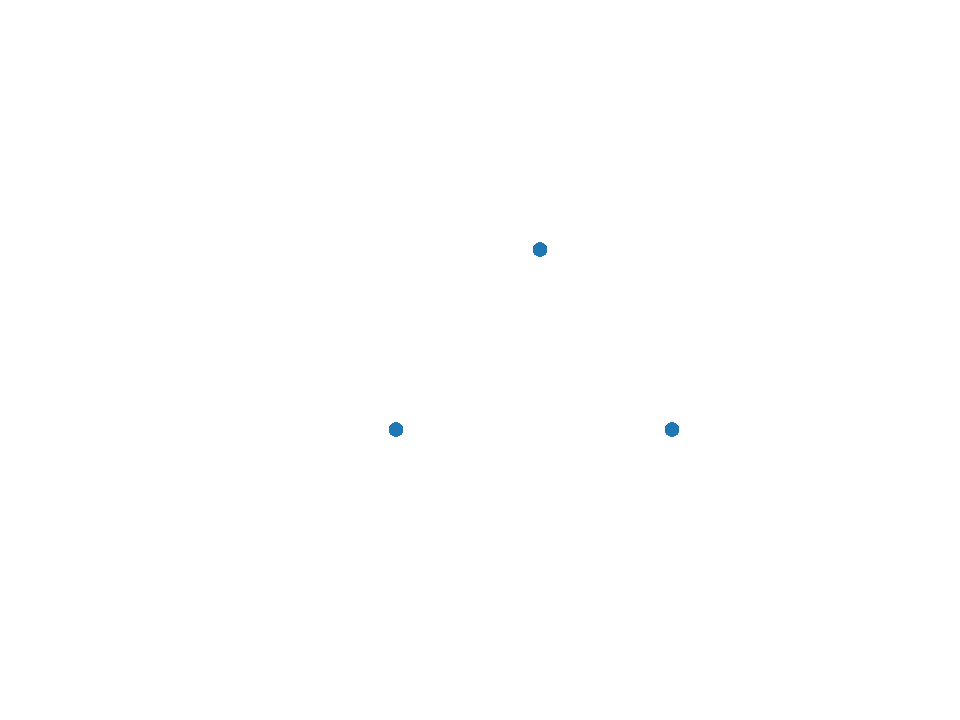
\includegraphics[scale=0.45]{figures/e1mwc1.pdf}}
	\only<2>{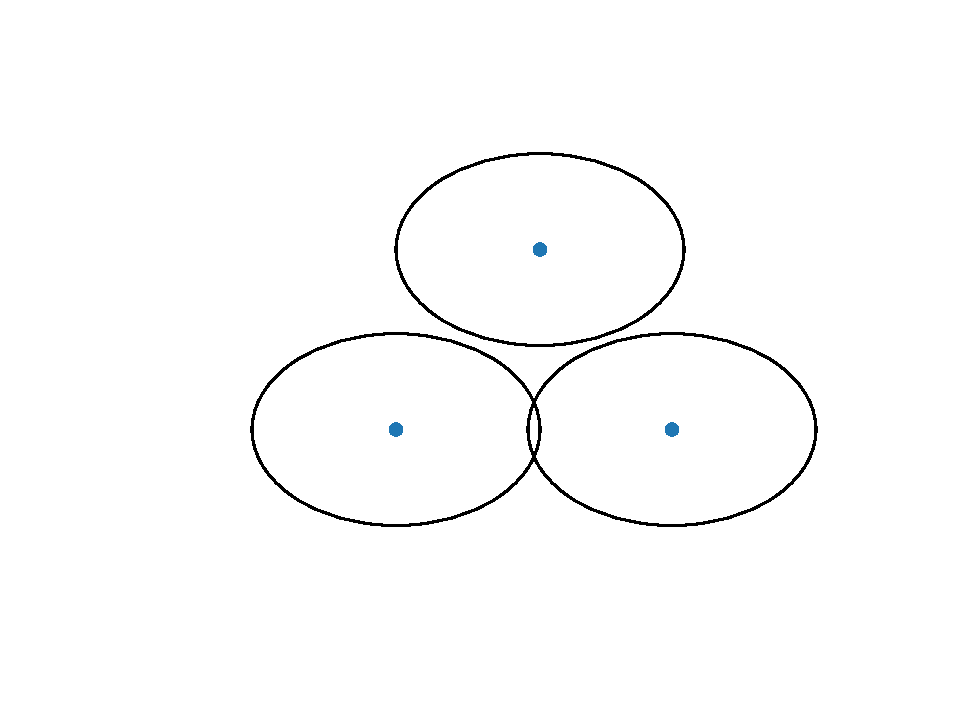
\includegraphics[scale=0.45]{figures/e1mwc2.pdf}}
	\only<3>{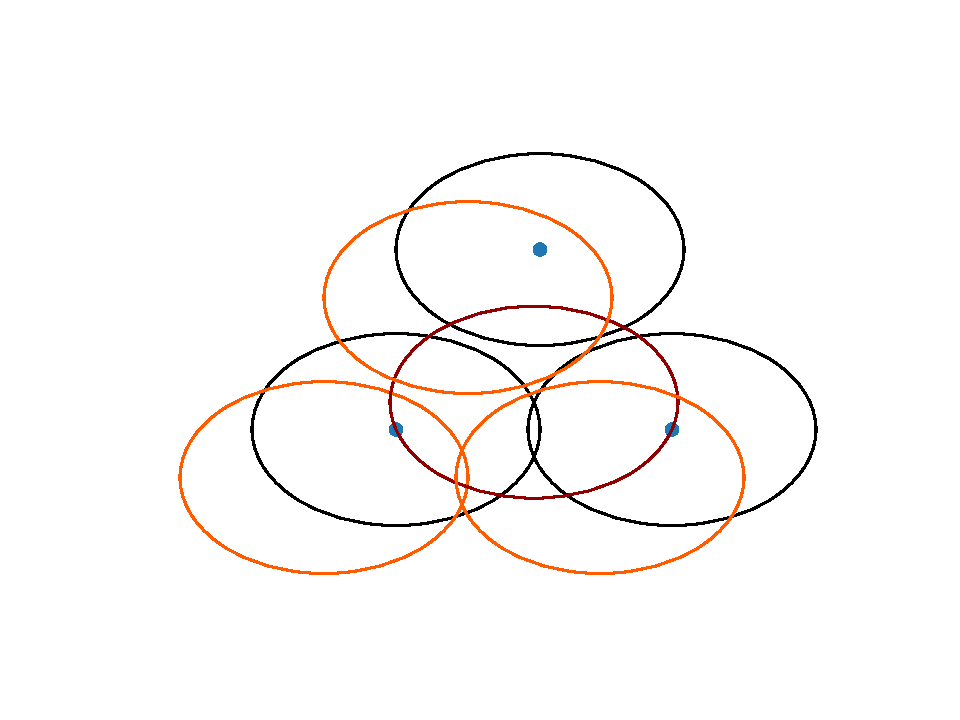
\includegraphics[scale=0.45]{figures/e1mwc3.pdf}}
	\only<4>{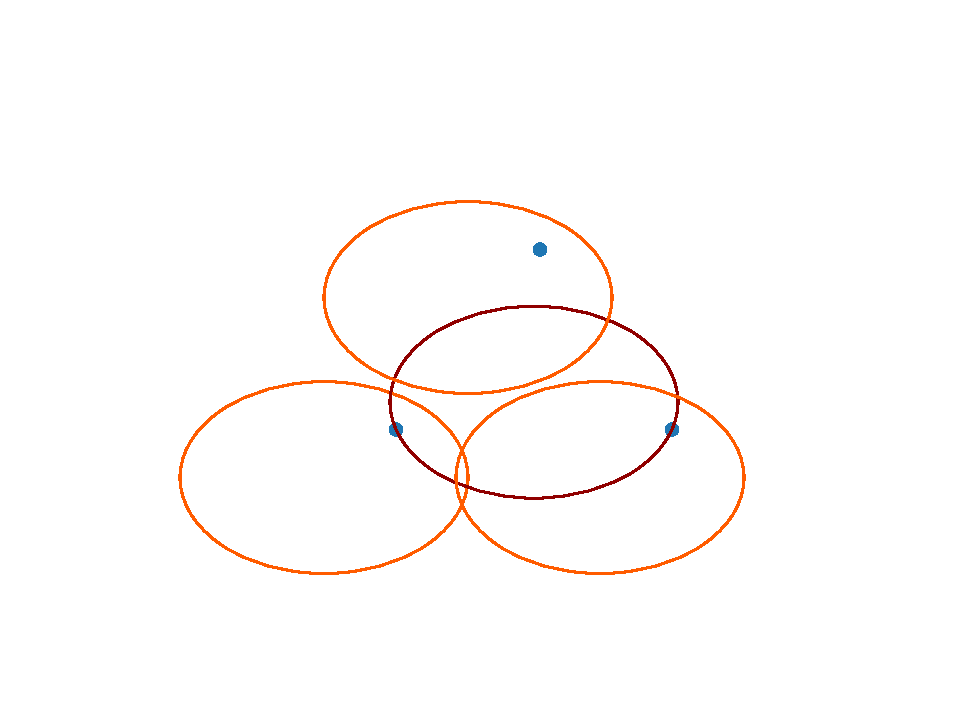
\includegraphics[scale=0.45]{figures/e1mwc4.pdf}}
	\only<5>{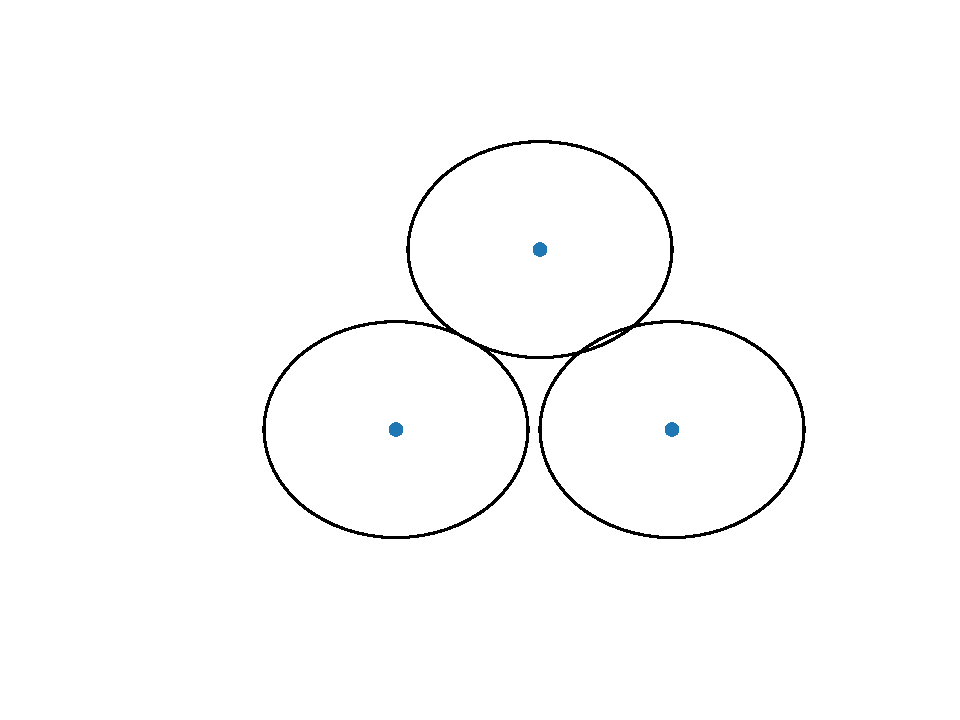
\includegraphics[scale=0.45]{figures/e2mwc2.pdf}}
	\only<6>{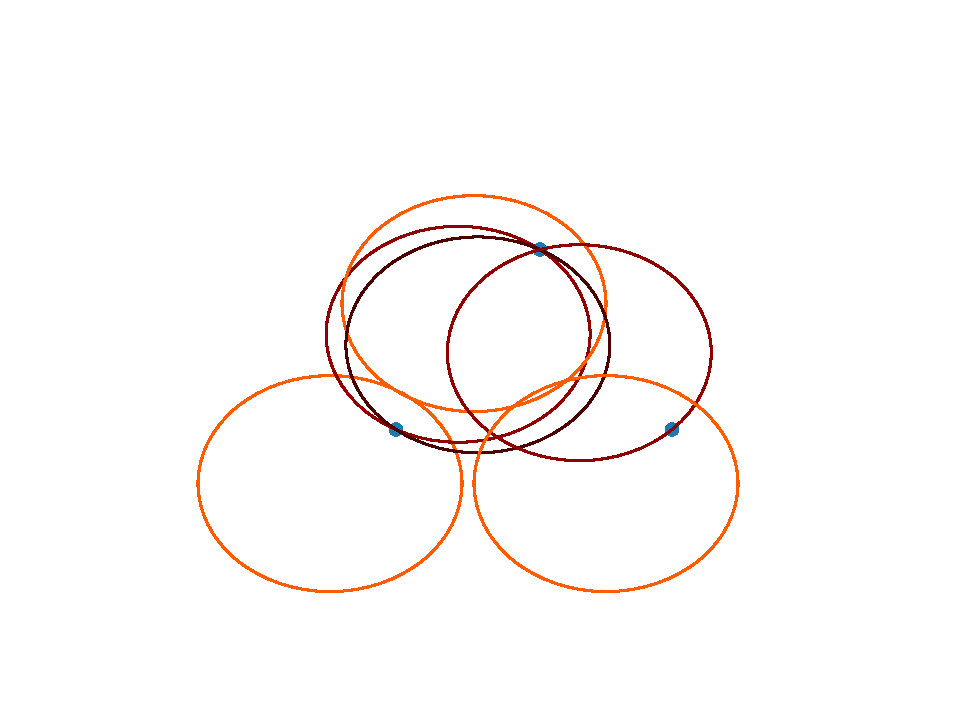
\includegraphics[scale=0.45]{figures/e2mwc4.pdf}}
	\only<7>{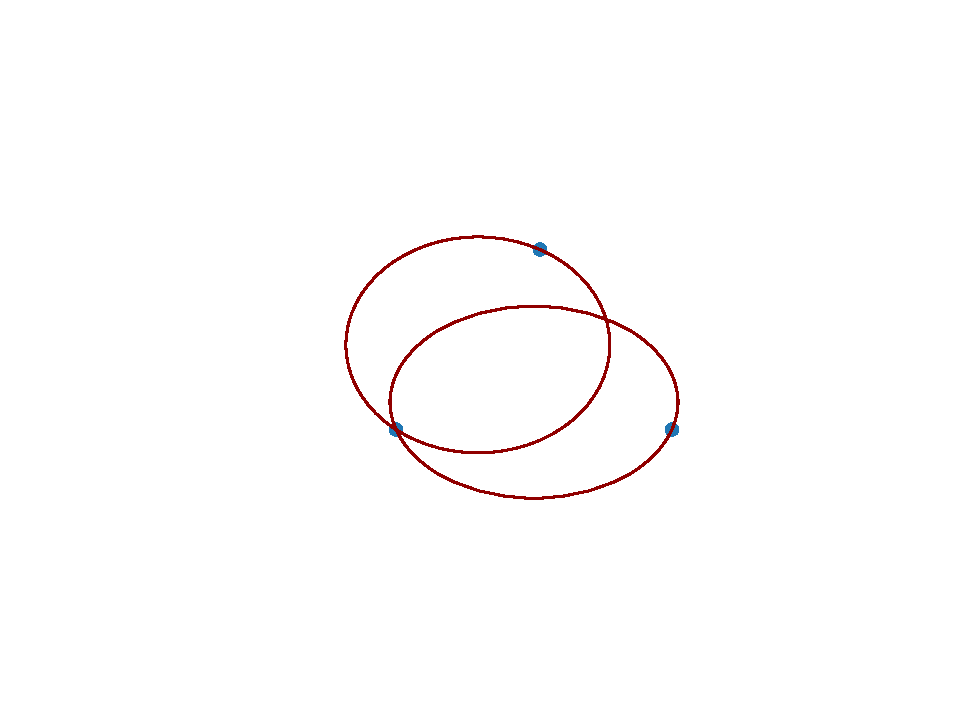
\includegraphics[scale=0.45]{figures/emopt.pdf}}
	
	\source{Elaborated by the author.}
\end{figure}
\end{frame}

\begin{frame}[fragile]{Maximal Covering by Ellipses}{The algorithm for $m$ ellipses}
	\begin{algorithm}[H]
		%\caption{Adaptation of the algorithm for one disk to produce a candidate list for every ellipse.}\label{algoritmo:mce1}
		\begin{algorithmic}[1]
			\FOR{$E_i \in \E$}
				\STATE{Fix an ellipse with the same shape as $E_i$ at each point.}
				\STATE{$Z_i \gets $ every solution of Maximum Weight Clique for it.}
			\ENDFOR
		\end{algorithmic}
	\end{algorithm}
\begin{algorithm}[H]
	\begin{algorithmic}[1]

			\STATE{\textbf{function} $f(\Pp, j)$}
				
				\IF{$j=m$}{
					\RETURN 0
				}
				\ENDIF
				\STATE{$ans \gets 0$}
				\FOR{$z \in Z_j$}
					\STATE{Fix $E_j$ at $z$}
					\STATE{$Q \gets$ points covered by $E_j(z)$}
					\STATE{$ans \gets \max\{ans,f(\Pp \setminus Q, j+1) + w(Q)\}$}
				\ENDFOR
				\RETURN{$ans$}
			
			
			%\FOR{$p_i \in \Pp$}
			%\STATE $A \gets \bigcup_{j \in I_i} \{\Gamma_+(i,j) \cup \Gamma_-(i,j)\}$
			%\STATE $Z \gets \{\}$
			%\STATE $Cov \gets \{p_i\}$
			%\FOR{$cnt=1..2$} 
			%\FOR{$a \in A$}
			%\STATE Let $p_a$ be the point that intersects $E_i$ at angle $a$. 
			%\IF{$a$ is a starting angle}
			%\STATE $Cov \gets Cov \cup \{p_a\}$
			%\ELSE
			%\STATE $Cov \gets Cov \setminus \{p_a\}$
			%\ENDIF
			%\STATE $Z \gets Z \cup \{Cov\}$
			%\ENDFOR
			%\ENDFOR
			%\ENDFOR
			
		\end{algorithmic}
	\end{algorithm}
\end{frame}

%\begin{frame}{Maximal Covering by Ellipses}{$m$ Ellipses}
%	The modified one-disk-cover algorithm produces a list of candidates of location for each ellipse. An optimal solution is guaranteed to be in this list.
%\end{frame}

%\begin{frame}
%	\begin{figure}
%		\caption{Optimal solution with two ellipses for a random instance.}
%		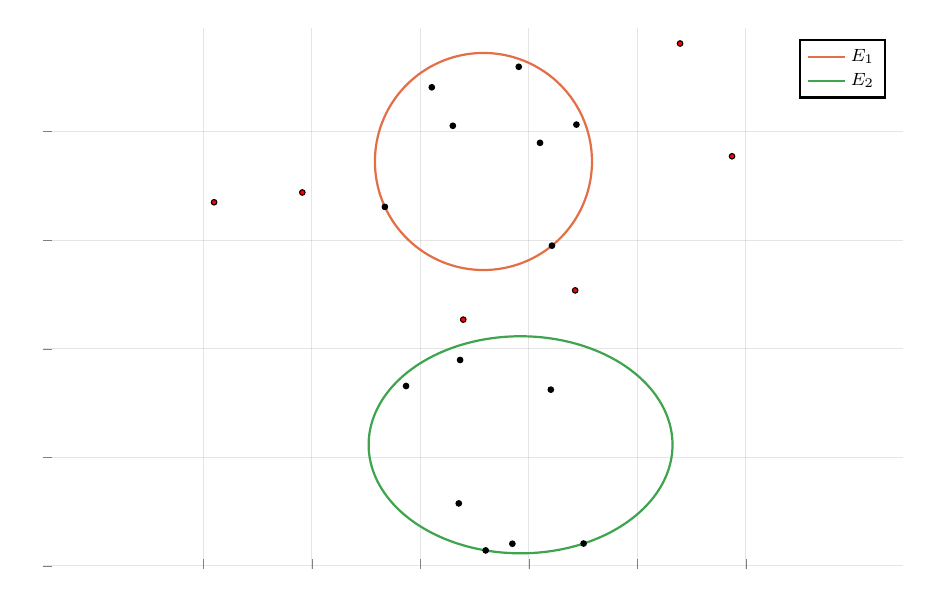
\begin{tikzpicture}[scale=0.8]
\begin{axis}[height = {101.6mm}, axis equal = {true}, ylabel = {}, xmin = {-0.04304650080536887}, xmax = {5.015893955055976}, ymax = {4.953655933510717}, xlabel = {}, unbounded coords=jump,scaled x ticks = false,xlabel style = {font = {\fontsize{11 pt}{14.3 pt}\selectfont}, color = {rgb,1:red,0.00000000;green,0.00000000;blue,0.00000000}, draw opacity = 1.0, rotate = 0.0},xmajorgrids = true,xtick = {0.0,1.0,2.0,3.0,4.0,5.0},xticklabels = {},xtick align = inside,xticklabel style = {font = {\fontsize{8 pt}{10.4 pt}\selectfont}, color = {rgb,1:red,0.00000000;green,0.00000000;blue,0.00000000}, draw opacity = 1.0, rotate = 0.0},x grid style = {color = {rgb,1:red,0.00000000;green,0.00000000;blue,0.00000000},
draw opacity = 0.1,
line width = 0.5,
solid},axis lines* = left,separate axis lines,x axis line style = {draw opacity = 0},scaled y ticks = false,ylabel style = {font = {\fontsize{11 pt}{14.3 pt}\selectfont}, color = {rgb,1:red,0.00000000;green,0.00000000;blue,0.00000000}, draw opacity = 1.0, rotate = 0.0},ymajorgrids = true,ytick = {0.0,1.0,2.0,3.0,4.0},yticklabels = {},ytick align = inside,yticklabel style = {font = {\fontsize{8 pt}{10.4 pt}\selectfont}, color = {rgb,1:red,0.00000000;green,0.00000000;blue,0.00000000}, draw opacity = 1.0, rotate = 0.0},y grid style = {color = {rgb,1:red,0.00000000;green,0.00000000;blue,0.00000000},
draw opacity = 0.1,
line width = 0.5,
solid},axis lines* = left,separate axis lines,y axis line style = {draw opacity = 0},    xshift = 0.0mm,
    yshift = 0.0mm,
    axis background/.style={fill={rgb,1:red,1.00000000;green,1.00000000;blue,1.00000000}}
,legend style = {color = {rgb,1:red,0.00000000;green,0.00000000;blue,0.00000000},
draw opacity = 1.0,
line width = 1,
solid,fill = {rgb,1:red,1.00000000;green,1.00000000;blue,1.00000000},font = {\fontsize{8 pt}{10.4 pt}\selectfont}},colorbar style={title=}, ymin = {-0.025453315895344608}, width = {152.4mm}]\addplot+[draw=none, color = {rgb,1:red,0.00000000;green,0.00000000;blue,0.00000000},
draw opacity = 1.0,
line width = 0,
solid,mark = *,
mark size = 1.25,
mark options = {
    color = {rgb,1:red,0.00000000;green,0.00000000;blue,0.00000000}, draw opacity = 1.0,
    fill = {rgb,1:red,0.00000000;green,0.00000000;blue,0.00000000}, fill opacity = 1.0,
    line width = 0.5,
    rotate = 0,
    solid
},forget plot] coordinates {
(2.602918949315934, 0.1421191370308239)
};
\addplot+[draw=none, color = {rgb,1:red,1.00000000;green,0.00000000;blue,0.00000000},
draw opacity = 1.0,
line width = 0,
solid,mark = *,
mark size = 1.25,
mark options = {
    color = {rgb,1:red,0.00000000;green,0.00000000;blue,0.00000000}, draw opacity = 1.0,
    fill = {rgb,1:red,1.00000000;green,0.00000000;blue,0.00000000}, fill opacity = 1.0,
    line width = 0.5,
    rotate = 0,
    solid
},forget plot] coordinates {
(2.396020400537423, 2.2686705873010817)
};
\addplot+[draw=none, color = {rgb,1:red,1.00000000;green,0.00000000;blue,0.00000000},
draw opacity = 1.0,
line width = 0,
solid,mark = *,
mark size = 1.25,
mark options = {
    color = {rgb,1:red,0.00000000;green,0.00000000;blue,0.00000000}, draw opacity = 1.0,
    fill = {rgb,1:red,1.00000000;green,0.00000000;blue,0.00000000}, fill opacity = 1.0,
    line width = 0.5,
    rotate = 0,
    solid
},forget plot] coordinates {
(4.872716394984428, 3.773817627065047)
};
\addplot+[draw=none, color = {rgb,1:red,0.00000000;green,0.00000000;blue,0.00000000},
draw opacity = 1.0,
line width = 0,
solid,mark = *,
mark size = 1.25,
mark options = {
    color = {rgb,1:red,0.00000000;green,0.00000000;blue,0.00000000}, draw opacity = 1.0,
    fill = {rgb,1:red,0.00000000;green,0.00000000;blue,0.00000000}, fill opacity = 1.0,
    line width = 0.5,
    rotate = 0,
    solid
},forget plot] coordinates {
(3.202948490978642, 1.6235525016076402)
};
\addplot+[draw=none, color = {rgb,1:red,0.00000000;green,0.00000000;blue,0.00000000},
draw opacity = 1.0,
line width = 0,
solid,mark = *,
mark size = 1.25,
mark options = {
    color = {rgb,1:red,0.00000000;green,0.00000000;blue,0.00000000}, draw opacity = 1.0,
    fill = {rgb,1:red,0.00000000;green,0.00000000;blue,0.00000000}, fill opacity = 1.0,
    line width = 0.5,
    rotate = 0,
    solid
},forget plot] coordinates {
(2.848573275272137, 0.20375192853344104)
};
\addplot+[draw=none, color = {rgb,1:red,0.00000000;green,0.00000000;blue,0.00000000},
draw opacity = 1.0,
line width = 0,
solid,mark = *,
mark size = 1.25,
mark options = {
    color = {rgb,1:red,0.00000000;green,0.00000000;blue,0.00000000}, draw opacity = 1.0,
    fill = {rgb,1:red,0.00000000;green,0.00000000;blue,0.00000000}, fill opacity = 1.0,
    line width = 0.5,
    rotate = 0,
    solid
},forget plot] coordinates {
(1.8690841880778053, 1.6568512573232197)
};
\addplot+[draw=none, color = {rgb,1:red,0.00000000;green,0.00000000;blue,0.00000000},
draw opacity = 1.0,
line width = 0,
solid,mark = *,
mark size = 1.25,
mark options = {
    color = {rgb,1:red,0.00000000;green,0.00000000;blue,0.00000000}, draw opacity = 1.0,
    fill = {rgb,1:red,0.00000000;green,0.00000000;blue,0.00000000}, fill opacity = 1.0,
    line width = 0.5,
    rotate = 0,
    solid
},forget plot] coordinates {
(2.300100178756294, 4.05463630589837)
};
\addplot+[draw=none, color = {rgb,1:red,0.00000000;green,0.00000000;blue,0.00000000},
draw opacity = 1.0,
line width = 0,
solid,mark = *,
mark size = 1.25,
mark options = {
    color = {rgb,1:red,0.00000000;green,0.00000000;blue,0.00000000}, draw opacity = 1.0,
    fill = {rgb,1:red,0.00000000;green,0.00000000;blue,0.00000000}, fill opacity = 1.0,
    line width = 0.5,
    rotate = 0,
    solid
},forget plot] coordinates {
(1.6738171002119706, 3.3074971831952427)
};
\addplot+[draw=none, color = {rgb,1:red,0.00000000;green,0.00000000;blue,0.00000000},
draw opacity = 1.0,
line width = 0,
solid,mark = *,
mark size = 1.25,
mark options = {
    color = {rgb,1:red,0.00000000;green,0.00000000;blue,0.00000000}, draw opacity = 1.0,
    fill = {rgb,1:red,0.00000000;green,0.00000000;blue,0.00000000}, fill opacity = 1.0,
    line width = 0.5,
    rotate = 0,
    solid
},forget plot] coordinates {
(2.907448354814198, 4.598195661337079)
};
\addplot+[draw=none, color = {rgb,1:red,1.00000000;green,0.00000000;blue,0.00000000},
draw opacity = 1.0,
line width = 0,
solid,mark = *,
mark size = 1.25,
mark options = {
    color = {rgb,1:red,0.00000000;green,0.00000000;blue,0.00000000}, draw opacity = 1.0,
    fill = {rgb,1:red,1.00000000;green,0.00000000;blue,0.00000000}, fill opacity = 1.0,
    line width = 0.5,
    rotate = 0,
    solid
},forget plot] coordinates {
(0.1001310592661786, 3.3500841191834887)
};
\addplot+[draw=none, color = {rgb,1:red,1.00000000;green,0.00000000;blue,0.00000000},
draw opacity = 1.0,
line width = 0,
solid,mark = *,
mark size = 1.25,
mark options = {
    color = {rgb,1:red,0.00000000;green,0.00000000;blue,0.00000000}, draw opacity = 1.0,
    fill = {rgb,1:red,1.00000000;green,0.00000000;blue,0.00000000}, fill opacity = 1.0,
    line width = 0.5,
    rotate = 0,
    solid
},forget plot] coordinates {
(0.9130732329791647, 3.4401427131346485)
};
\addplot+[draw=none, color = {rgb,1:red,0.00000000;green,0.00000000;blue,0.00000000},
draw opacity = 1.0,
line width = 0,
solid,mark = *,
mark size = 1.25,
mark options = {
    color = {rgb,1:red,0.00000000;green,0.00000000;blue,0.00000000}, draw opacity = 1.0,
    fill = {rgb,1:red,0.00000000;green,0.00000000;blue,0.00000000}, fill opacity = 1.0,
    line width = 0.5,
    rotate = 0,
    solid
},forget plot] coordinates {
(3.4385814568108195, 4.065543992107185)
};
\addplot+[draw=none, color = {rgb,1:red,0.00000000;green,0.00000000;blue,0.00000000},
draw opacity = 1.0,
line width = 0,
solid,mark = *,
mark size = 1.25,
mark options = {
    color = {rgb,1:red,0.00000000;green,0.00000000;blue,0.00000000}, draw opacity = 1.0,
    fill = {rgb,1:red,0.00000000;green,0.00000000;blue,0.00000000}, fill opacity = 1.0,
    line width = 0.5,
    rotate = 0,
    solid
},forget plot] coordinates {
(2.354854569358288, 0.5753620833645212)
};
\addplot+[draw=none, color = {rgb,1:red,1.00000000;green,0.00000000;blue,0.00000000},
draw opacity = 1.0,
line width = 0,
solid,mark = *,
mark size = 1.25,
mark options = {
    color = {rgb,1:red,0.00000000;green,0.00000000;blue,0.00000000}, draw opacity = 1.0,
    fill = {rgb,1:red,1.00000000;green,0.00000000;blue,0.00000000}, fill opacity = 1.0,
    line width = 0.5,
    rotate = 0,
    solid
},forget plot] coordinates {
(4.393915159418624, 4.812737747206772)
};
\addplot+[draw=none, color = {rgb,1:red,0.00000000;green,0.00000000;blue,0.00000000},
draw opacity = 1.0,
line width = 0,
solid,mark = *,
mark size = 1.25,
mark options = {
    color = {rgb,1:red,0.00000000;green,0.00000000;blue,0.00000000}, draw opacity = 1.0,
    fill = {rgb,1:red,0.00000000;green,0.00000000;blue,0.00000000}, fill opacity = 1.0,
    line width = 0.5,
    rotate = 0,
    solid
},forget plot] coordinates {
(3.50505217637773, 0.20556942673409795)
};
\addplot+[draw=none, color = {rgb,1:red,1.00000000;green,0.00000000;blue,0.00000000},
draw opacity = 1.0,
line width = 0,
solid,mark = *,
mark size = 1.25,
mark options = {
    color = {rgb,1:red,0.00000000;green,0.00000000;blue,0.00000000}, draw opacity = 1.0,
    fill = {rgb,1:red,1.00000000;green,0.00000000;blue,0.00000000}, fill opacity = 1.0,
    line width = 0.5,
    rotate = 0,
    solid
},forget plot] coordinates {
(3.427160885660112, 2.538013336230315)
};
\addplot+[draw=none, color = {rgb,1:red,0.00000000;green,0.00000000;blue,0.00000000},
draw opacity = 1.0,
line width = 0,
solid,mark = *,
mark size = 1.25,
mark options = {
    color = {rgb,1:red,0.00000000;green,0.00000000;blue,0.00000000}, draw opacity = 1.0,
    fill = {rgb,1:red,0.00000000;green,0.00000000;blue,0.00000000}, fill opacity = 1.0,
    line width = 0.5,
    rotate = 0,
    solid
},forget plot] coordinates {
(2.1063177109467004, 4.409416548982065)
};
\addplot+[draw=none, color = {rgb,1:red,0.00000000;green,0.00000000;blue,0.00000000},
draw opacity = 1.0,
line width = 0,
solid,mark = *,
mark size = 1.25,
mark options = {
    color = {rgb,1:red,0.00000000;green,0.00000000;blue,0.00000000}, draw opacity = 1.0,
    fill = {rgb,1:red,0.00000000;green,0.00000000;blue,0.00000000}, fill opacity = 1.0,
    line width = 0.5,
    rotate = 0,
    solid
},forget plot] coordinates {
(2.3672535618848976, 1.8968192015410446)
};
\addplot+[draw=none, color = {rgb,1:red,0.00000000;green,0.00000000;blue,0.00000000},
draw opacity = 1.0,
line width = 0,
solid,mark = *,
mark size = 1.25,
mark options = {
    color = {rgb,1:red,0.00000000;green,0.00000000;blue,0.00000000}, draw opacity = 1.0,
    fill = {rgb,1:red,0.00000000;green,0.00000000;blue,0.00000000}, fill opacity = 1.0,
    line width = 0.5,
    rotate = 0,
    solid
},forget plot] coordinates {
(3.213442183570654, 2.9502323475574324)
};
\addplot+[draw=none, color = {rgb,1:red,0.00000000;green,0.00000000;blue,0.00000000},
draw opacity = 1.0,
line width = 0,
solid,mark = *,
mark size = 1.25,
mark options = {
    color = {rgb,1:red,0.00000000;green,0.00000000;blue,0.00000000}, draw opacity = 1.0,
    fill = {rgb,1:red,0.00000000;green,0.00000000;blue,0.00000000}, fill opacity = 1.0,
    line width = 0.5,
    rotate = 0,
    solid
},forget plot] coordinates {
(3.1034740796888682, 3.8975002907243397)
};
\addplot+ [color = {rgb,1:red,0.88887350;green,0.43564919;blue,0.27812294},
draw opacity = 1.0,
line width = 1,
solid,mark = none,
mark size = 2.0,
mark options = {
    color = {rgb,1:red,0.00000000;green,0.00000000;blue,0.00000000}, draw opacity = 1.0,
    fill = {rgb,1:red,0.88887350;green,0.43564919;blue,0.27812294}, fill opacity = 1.0,
    line width = 1,
    rotate = 0,
    solid
}]coordinates {
(3.5821391801246905, 3.725768625135797)
(3.581640769250864, 3.7573371749006075)
(3.5801460334561837, 3.7888742564484703)
(3.5776564627257965, 3.8203484329306416)
(3.574174538717948, 3.8517283302035143)
(3.5697037322902143, 3.8829826681030477)
(3.564248500039671, 3.9140802916255146)
(3.557814279860464, 3.9449902019834884)
(3.5504074855231975, 3.9756815875061053)
(3.5420355002815476, 4.006123854352811)
(3.532706669512473, 4.036286657009966)
(3.522430292397366, 4.06613992853991)
(3.511216612652421, 4.095653910552343)
(3.4990768083174792, 4.124799182868138)
(3.486022980613514, 4.153546692846007)
(3.4720681418798707, 4.1818677843428125)
(3.4572262026032843, 4.209734226278636)
(3.4415119575516027, 4.237118240778123)
(3.424941071026041, 4.263992530860086)
(3.407530061246667, 4.290330307647715)
(3.389296283886676, 4.316105317072325)
(3.3702579147718827, 4.341291866043976)
(3.3504339317626615, 4.365864848062904)
(3.3298440958363997, 4.389799768246228)
(3.30850893138933, 4.413072767744981)
(3.2864497057773625, 4.43566064752713)
(3.2636884081163244, 4.457540891502873)
(3.2402477273627284, 4.478691688969174)
(3.2161510296969293, 4.499091956351136)
(3.191422335231207, 4.518721358218576)
(3.166086294065997, 4.537560327556817)
(3.1401681617181305, 4.555590085271523)
(3.1136937739455917, 4.572792658908096)
(3.086689520993868, 4.58915090056702)
(3.05918232128958, 4.604648503997257)
(3.0311995946076107, 4.619270020850671)
(3.0027692347384747, 4.633000876081278)
(2.973919581683184, 4.645827382473971)
(2.944679393403315, 4.657736754288232)
(2.9150778171544514, 4.668717120003234)
(2.885144360431563, 4.678757534151636)
(2.8549088615552938, 4.68784798823026)
(2.8244014599284735, 4.6959794206767835)
(2.7936525659925096, 4.703143725902504)
(2.762692830913593, 4.709333762372166)
(2.7315531160289512, 4.7145433597228)
(2.7002644620835987, 4.718767324914467)
(2.6688580582882415, 4.722001447406804)
(2.6373652112291985, 4.724242503356176)
(2.6058173136613147, 4.725488258829275)
(2.574245813214977, 4.725737472029953)
(2.5426821810484377, 4.724989894537073)
(2.5111578804766745, 4.723246271552136)
(2.4797043356080772, 4.720508341156454)
(2.4483529000202116, 4.716778832578589)
(2.4171348255058915, 4.7120614634738)
(2.3860812309207127, 4.706360936218201)
(2.3552230711631004, 4.699682933221335)
(2.3245911063177935, 4.692034111261819)
(2.294215870993524, 4.683422094851727)
(2.2641276438854523, 4.673855468636306)
(2.234356417592708, 4.663343768836622)
(2.2049318687211144, 4.651897473743638)
(2.175883328300902, 4.639527993273234)
(2.1472397525488973, 4.626247657592549)
(2.1190296940043427, 4.612069704829006)
(2.091281273067097, 4.597008267874257)
(2.0640221499666134, 4.581078360296209)
(2.03727949718962, 4.564295861373174)
(2.0110799723939956, 4.5466775002650595)
(1.9854496918358344, 4.528240839337375)
(1.9604142043361954, 4.509004256654688)
(1.9359984658134808, 4.4889869276609655)
(1.9122268144068353, 4.46820880606508)
(1.8891229462153587, 4.446690603950513)
(1.8667098916773193, 4.424453771129103)
(1.8450099926129115, 4.401520473759406)
(1.824044879953445, 4.377913572250984)
(1.8038354521791604, 4.353656598476655)
(1.7844018544871711, 4.328773732315412)
(1.7657634587102913, 4.303289777549385)
(1.747938844006773, 4.277230137138904)
(1.730945778340196, 4.2506207879002655)
(1.714801200767976, 4.22348825461148)
(1.6995212045561434, 4.1958595835718)
(1.685121021137227, 4.167762315641376)
(1.6716150049272283, 4.139224458787931)
(1.6590166190168298, 4.110274460167808)
(1.6473384217510922, 4.080941177769225)
(1.6365920542110235, 4.051253851646009)
(1.6267882286094957, 4.021242074770467)
(1.6179367176130788, 3.9909357635344755)
(1.6100463446004336, 3.9603651279281658)
(1.603124974866976, 3.929560641425949)
(1.59717950778458, 3.8985530106098967)
(1.5922158699241333, 3.8673731445607484)
(1.5882390091478027, 3.8360521240470717)
(1.5852528896768971, 3.8046211705432733)
(1.583260488140247, 3.773111615107355)
(1.5822637906070331, 3.7415548671494343)
(1.5822637906070331, 3.70998238312216)
(1.583260488140247, 3.678425635164239)
(1.5852528896768971, 3.6469160797283204)
(1.5882390091478027, 3.615485126224522)
(1.592215869924133, 3.5841641057108458)
(1.5971795077845798, 3.552984239661697)
(1.6031249748669758, 3.5219766088456446)
(1.6100463446004336, 3.4911721223434284)
(1.6179367176130786, 3.460601486737118)
(1.6267882286094957, 3.430295175501127)
(1.6365920542110233, 3.4002833986255854)
(1.6473384217510922, 3.3705960725023685)
(1.6590166190168296, 3.3412627901037864)
(1.6716150049272283, 3.312312791483663)
(1.6851210211372267, 3.283774934630218)
(1.6995212045561434, 3.255677666699794)
(1.7148012007679758, 3.2280489956601137)
(1.7309457783401958, 3.2009164623713287)
(1.747938844006773, 3.1743071131326897)
(1.7657634587102913, 3.1482474727222085)
(1.784401854487171, 3.122763517956183)
(1.8038354521791602, 3.097880651794939)
(1.824044879953445, 3.0736236780206103)
(1.8450099926129115, 3.050016776512188)
(1.866709891677319, 3.0270834791424903)
(1.8891229462153585, 3.004846646321081)
(1.912226814406835, 2.983328444206514)
(1.9359984658134803, 2.9625503226106287)
(1.9604142043361952, 2.9425329936169065)
(1.985449691835834, 2.923296410934219)
(2.0110799723939956, 2.9048597500065343)
(2.03727949718962, 2.8872413888984196)
(2.064022149966613, 2.870458889975385)
(2.091281273067097, 2.8545289823973374)
(2.1190296940043423, 2.8394675454425884)
(2.1472397525488973, 2.825289592679045)
(2.175883328300902, 2.81200925699836)
(2.204931868721114, 2.7996397765279557)
(2.234356417592708, 2.7881934814349716)
(2.264127643885452, 2.7776817816352875)
(2.294215870993524, 2.7681151554198675)
(2.324591106317794, 2.759503139009775)
(2.3552230711631, 2.751854317050259)
(2.3860812309207122, 2.745176314053393)
(2.4171348255058906, 2.739475786797794)
(2.448352900020211, 2.734758417693005)
(2.4797043356080772, 2.73102890911514)
(2.511157880476674, 2.7282909787194582)
(2.5426821810484377, 2.726547355734521)
(2.5742458132149766, 2.7257997782416403)
(2.6058173136613143, 2.726048991442319)
(2.637365211229199, 2.727294746915418)
(2.668858058288241, 2.72953580286479)
(2.7002644620835987, 2.732769925357127)
(2.731553116028951, 2.7369938905487943)
(2.7626928309135925, 2.742203487899427)
(2.7936525659925096, 2.7483935243690896)
(2.8244014599284735, 2.7555578295948107)
(2.8549088615552938, 2.763689262041334)
(2.8851443604315627, 2.7727797161199574)
(2.9150778171544514, 2.7828201302683597)
(2.944679393403314, 2.793800495983362)
(2.9739195816831834, 2.8057098677976224)
(3.0027692347384747, 2.8185363741903156)
(3.0311995946076102, 2.8322672294209226)
(3.05918232128958, 2.8468887462743364)
(3.0866895209938674, 2.862386349704573)
(3.1136937739455917, 2.878744591363498)
(3.1401681617181305, 2.895947165000071)
(3.1660862940659964, 2.913976922714776)
(3.191422335231207, 2.9328158920530183)
(3.2161510296969285, 2.9524452939204573)
(3.240247727362728, 2.9728455613024196)
(3.2636884081163244, 2.99399635876872)
(3.2864497057773625, 3.0158766027444637)
(3.30850893138933, 3.0384644825266127)
(3.3298440958363993, 3.0617374820253653)
(3.350433931762661, 3.0856724022086897)
(3.3702579147718827, 3.1102453842276176)
(3.389296283886676, 3.135431933199268)
(3.407530061246667, 3.161206942623879)
(3.4249410710260406, 3.187544719411508)
(3.441511957551602, 3.21441900949347)
(3.4572262026032843, 3.2418030239929583)
(3.4720681418798707, 3.2696694659287804)
(3.486022980613514, 3.2979905574255874)
(3.4990768083174792, 3.3267380674034555)
(3.511216612652421, 3.35588333971925)
(3.522430292397366, 3.3853973217316833)
(3.532706669512473, 3.4152505932616277)
(3.5420355002815476, 3.4454133959187825)
(3.5504074855231975, 3.475855662765488)
(3.557814279860464, 3.5065470482881054)
(3.5642485000396706, 3.5374569586460782)
(3.569703732290214, 3.568554582168546)
(3.574174538717948, 3.5998089200680794)
(3.5776564627257965, 3.6311888173409517)
(3.5801460334561837, 3.662662993823123)
(3.581640769250864, 3.694200075370986)
(3.5821391801246905, 3.7257686251357964)
};
\addlegendentry{$E_1$}
\addplot+ [color = {rgb,1:red,0.24222430;green,0.64327509;blue,0.30444865},
draw opacity = 1.0,
line width = 1,
solid,mark = none,
mark size = 2.0,
mark options = {
    color = {rgb,1:red,0.00000000;green,0.00000000;blue,0.00000000}, draw opacity = 1.0,
    fill = {rgb,1:red,0.24222430;green,0.64327509;blue,0.30444865}, fill opacity = 1.0,
    line width = 1,
    rotate = 0,
    solid
}]coordinates {
(4.324183803520279, 1.1154337173027569)
(4.323486028296922, 1.1470022670675675)
(4.3213933981843695, 1.1785393486154305)
(4.317907999161827, 1.2100135250976018)
(4.31303330555084, 1.2413934223704743)
(4.306774176552012, 1.2726477602700077)
(4.299136851401252, 1.3037453837924748)
(4.290128943150362, 1.3346552941504481)
(4.279759431078189, 1.3653466796730651)
(4.268038651739879, 1.3957889465197713)
(4.254978288663175, 1.4259517491769258)
(4.240591360702025, 1.4558050207068698)
(4.224892209059101, 1.4853190027193037)
(4.207896482990183, 1.5144642750350978)
(4.189621124204632, 1.5432117850129665)
(4.1700843499775315, 1.5715328765097727)
(4.14930563499031, 1.5993993184455957)
(4.127305691917956, 1.6267833329450836)
(4.10410645078217, 1.6536576230270454)
(4.079731037091046, 1.679995399814675)
(4.054203748787058, 1.7057704092392854)
(4.027550032026348, 1.730956958210936)
(3.999796455813438, 1.7555299402298639)
(3.9709706855166718, 1.7794648604131882)
(3.941101455290774, 1.8027378599119412)
(3.9102185394340196, 1.8253257396940898)
(3.8783527227085663, 1.8472059836698336)
(3.8455357696535315, 1.868356781136134)
(3.811800392921413, 1.8887570485180958)
(3.7771802206694023, 1.9083864503855354)
(3.7417097630381075, 1.9272254197237775)
(3.705424377751095, 1.9452551774384825)
(3.668360234869541, 1.9624577510750556)
(3.6305542807371274, 1.9788159927339801)
(3.592044201151124, 1.994313596164217)
(3.5528683837963673, 2.008935113017631)
(3.5130658799795773, 2.022665968248238)
(3.4726763657021693, 2.0354924746409315)
(3.4317401021103535, 2.0474018464551915)
(3.3902978953619445, 2.058382212170194)
(3.3483910559499006, 2.068422626318596)
(3.3060613575231232, 2.0775130803972197)
(3.2633509952455753, 2.0856445128437433)
(3.2203025437352255, 2.092808818069464)
(3.176958914624742, 2.0989988545391265)
(3.133363313786244, 2.1042084518897592)
(3.08955919826275, 2.1084324170814264)
(3.0455902329492504, 2.1116665395737635)
(3.0015002470665904, 2.113907595523136)
(2.9573331904715525, 2.115153350996235)
(2.9131330898466805, 2.115402564196913)
(2.868944004813525, 2.1146549867040325)
(2.824809984013057, 2.1129113637190957)
(2.7807750211970204, 2.1101734333234137)
(2.736883011374008, 2.106443924745549)
(2.69317770705396, 2.1017265556407594)
(2.64970267463471, 2.096026028385161)
(2.606501250974053, 2.089348025388295)
(2.5636165001906237, 2.0816992034287787)
(2.521091170736646, 2.0730871870186864)
(2.4789676527853457, 2.0635205608032665)
(2.4372879359755037, 2.053008861003582)
(2.3960935675552726, 2.0415625659105983)
(2.3554256109669747, 2.029193085440194)
(2.315324604914169, 2.0159127497595084)
(2.275830522951792, 2.0017347969959656)
(2.236982733639648, 1.9866733600412165)
(2.198819961298971, 1.9707434524631688)
(2.1613802474111803, 1.9539609535401343)
(2.1247009126973064, 1.9363425924320194)
(2.088818519915881, 1.9179059315043347)
(2.053768837416386, 1.8986693488216475)
(2.019586803484586, 1.8786520198279255)
(1.9863064915152817, 1.85787389823204)
(1.9539610760472146, 1.8363556961174732)
(1.9225827996939593, 1.8141188632960634)
(1.8922029410037886, 1.7911855659263658)
(1.8628517832805356, 1.7675786644179436)
(1.834558584396537, 1.743321690643615)
(1.807351547627752, 1.7184388244823714)
(1.7812577935401204, 1.6929548697163455)
(1.7563033329551947, 1.6668952293058643)
(1.7325130410219867, 1.6402858800672253)
(1.7099106324208786, 1.6131533467784402)
(1.6885186377243133, 1.5855246757387598)
(1.6683583809378302, 1.557427407808336)
(1.649449958243832, 1.528889550954891)
(1.6318122179692742, 1.4999395523347678)
(1.6154627417972416, 1.4706062699361855)
(1.6004178272411451, 1.4409189438129686)
(1.5866924713990063, 1.410907166937427)
(1.5743003560040227, 1.3806008557014355)
(1.5632538337863193, 1.3500302200951257)
(1.5535639161594788, 1.3192257335929092)
(1.5452402622441246, 1.2882181027768567)
(1.5382911692394992, 1.2570382367277084)
(1.5327235641526362, 1.225717216214032)
(1.5285429968933686, 1.1942862627102335)
(1.525753634742058, 1.1627767072743151)
(1.5243582581955588, 1.131219959316394)
(1.5243582581955588, 1.0996474752891199)
(1.525753634742058, 1.0680907273311988)
(1.5285429968933686, 1.0365811718952804)
(1.532723564152636, 1.005150218391482)
(1.538291169239499, 0.9738291978778055)
(1.5452402622441244, 0.9426493318286573)
(1.5535639161594788, 0.9116417010126048)
(1.5632538337863193, 0.8808372145103882)
(1.5743003560040225, 0.8502665789040784)
(1.5866924713990063, 0.819960267668087)
(1.600417827241145, 0.7899484907925455)
(1.6154627417972414, 0.7602611646693285)
(1.631812217969274, 0.7309278822707461)
(1.649449958243832, 0.701977883650623)
(1.66835838093783, 0.673440026797178)
(1.688518637724313, 0.6453427588667542)
(1.7099106324208786, 0.6177140878270737)
(1.7325130410219864, 0.5905815545382885)
(1.7563033329551945, 0.5639722052996495)
(1.7812577935401201, 0.5379125648891684)
(1.8073515476277517, 0.5124286101231426)
(1.8345585843965369, 0.48754574396189876)
(1.8628517832805351, 0.4632887701875703)
(1.8922029410037884, 0.43968186867914816)
(1.922582799693959, 0.41674857130945053)
(1.9539610760472144, 0.39451173848804066)
(1.9863064915152815, 0.372993536373474)
(2.019586803484585, 0.35221541477758866)
(2.053768837416386, 0.33219808578386645)
(2.08881851991588, 0.3129615031011793)
(2.124700912697306, 0.2945248421734944)
(2.1613802474111807, 0.2769064810653794)
(2.19881996129897, 0.2601239821423452)
(2.236982733639648, 0.24419407456429731)
(2.2758305229517912, 0.2291326376095485)
(2.3153246049141685, 0.21495468484600533)
(2.3554256109669747, 0.20167434916532012)
(2.396093567555272, 0.1893048686949158)
(2.4372879359755037, 0.1778585736019318)
(2.478967652785345, 0.16734687380224755)
(2.5210911707366455, 0.1577802475868274)
(2.5636165001906237, 0.14916823117673494)
(2.6065012509740524, 0.14151940921721917)
(2.64970267463471, 0.1348414062203528)
(2.6931777070539593, 0.12914087896475424)
(2.736883011374008, 0.12442350985996475)
(2.780775021197021, 0.12069400128209984)
(2.824809984013056, 0.11795607088641813)
(2.868944004813525, 0.11621244790148122)
(2.9131330898466796, 0.11546487040860054)
(2.9573331904715525, 0.11571408360927893)
(3.001500247066591, 0.11695983908237806)
(3.0455902329492495, 0.11920089503175013)
(3.08955919826275, 0.12243501752408725)
(3.1333633137862438, 0.12665898271575426)
(3.176958914624742, 0.1318685800663869)
(3.220302543735226, 0.13805861653604967)
(3.263350995245575, 0.14522292176177054)
(3.3060613575231232, 0.15335435420829402)
(3.3483910559499, 0.16244480828691743)
(3.3902978953619445, 0.17248522243531983)
(3.4317401021103526, 0.18346558815032177)
(3.472676365702169, 0.19537495996458232)
(3.513065879979577, 0.20820146635727554)
(3.5528683837963664, 0.22193232158788256)
(3.592044201151124, 0.23655383844129652)
(3.6305542807371265, 0.25205144187153317)
(3.6683602348695405, 0.2684096835304579)
(3.705424377751095, 0.2856122571670311)
(3.741709763038107, 0.3036420148817359)
(3.7771802206694023, 0.3224809842199783)
(3.8118003929214126, 0.3421103860874174)
(3.8455357696535315, 0.3625106534693797)
(3.8783527227085663, 0.38366145093568016)
(3.9102185394340196, 0.40554169491142367)
(3.9411014552907737, 0.4281295746935726)
(3.9709706855166713, 0.4514025741923252)
(3.9997964558134376, 0.47533749437564954)
(4.027550032026348, 0.49991047639457786)
(4.054203748787058, 0.5250970253662282)
(4.079731037091046, 0.5508720347908388)
(4.10410645078217, 0.5772098115784678)
(4.127305691917956, 0.60408410166043)
(4.14930563499031, 0.6314681161599183)
(4.170084349977531, 0.6593345580957406)
(4.189621124204632, 0.6876556495925473)
(4.207896482990183, 0.7164031595704154)
(4.224892209059101, 0.7455484318862099)
(4.240591360702025, 0.7750624138986434)
(4.254978288663175, 0.8049156854285877)
(4.268038651739879, 0.8350784880857425)
(4.279759431078189, 0.8655207549324481)
(4.290128943150362, 0.8962121404550654)
(4.299136851401252, 0.9271220508130384)
(4.306774176552012, 0.9582196743355058)
(4.31303330555084, 0.9894740122350394)
(4.317907999161827, 1.0208539095079114)
(4.3213933981843695, 1.0523280859900832)
(4.323486028296922, 1.0838651675379458)
(4.324183803520279, 1.1154337173027566)
};
\addlegendentry{$E_2$}
\end{axis}

\end{tikzpicture}

%		\source{Elaborated by the author.}
%	\end{figure}
%\end{frame}

\begin{frame}{Maximal Covering by Ellipses}
	
	\begin{itemize}
		\item The algorithm for $m$ ellipses tries every possible assignment of coverage for every one of the ellipses.
		\item Run-time complexity of $\bigO(n^{2m})$.
		
		\item Simpler than the $m$ disks algorithm proposed by \autocite{cabello:2006}. Achieves a similar complexity ($\bigO(n^{2m-1})$).
		
		\item Small improvements can be made in the pre-processing exhibited earlier in oder to reduce the size of the search space:
		\begin{itemize}
			\item Non-maximal coverage sets.
			%\item Ellipses that are too distant do not need to be checked.
		\end{itemize}
	
		%\item The unit-weight assumption can be easily dropped.
	\end{itemize}
	
\end{frame}




\section{Future Work}

\begin{frame}{Future Work}
	Primary goals:
\begin{itemize}
	\item Study the $(1-\epsilon)$-approximation method for the planar covering with disks in \autocite{cabello:2006} and develop an adapted version of the algorithm for ellipses with the same time complexity of $\bigO(n\log{n})$.
	
	\item Develop an exact method for the version of the problem introduced in \autocite{andreta} where the ellipses can be freely rotated.
\end{itemize}
\end{frame}

\begin{frame}{Future Work}
	
	Secondary goals:
	\begin{itemize}
		 

	\item Develop a probabilistic approximation algorithm based on \autocite{aronov:2008} which proposed a Monte Carlo approximation for the problem of finding the deepest point in a arrangement of regions. The method runs in $\bigO(n\epsilon^2\log{n})$ and can be applied to solve the case with one ellipse. The case with more than one ellipse is left as a challenge for us for the next steps of our research.
	
	\item In \autocite{zhou}, the task of finding every center candidate, after eliminating all the non-essential ones, is done in $\bigO(n^5)$ run-time complexity. We want to generalize this for the elliptical distance function and achieve a better run-time complexity. We also intend to use the mean-shift algorithm to try to develop a greedy version for the ellipses version.
	
		\end{itemize}
\end{frame}

\begin{frame}[allowframebreaks]
%	\frametitle{References}
%\bibliographystyle{authoryear-comp}
%	\bibliography{../references.bib}
\printbibliography
\end{frame}

\end{document}